\chapter{The Final Product}

I was able to stay on track with my schedule, implementing all aspects of my project that I had planned. Along the way, I learned how to add entitlements, ensuring my app had the necessary permissions and capabilities. Understanding HealthKit permissions and data handling was crucial for integrating health-related features seamlessly. Additionally, I gained insights into the differences between previewing, simulating, and deploying on an actual device, optimizing my app's performance for various environments. Moreover, I tackled the challenge of persisting images effectively, enhancing the user experience by securely storing visual data.

\section{Differences Between Prototype and Final Product}

Although the final version of my application remains faithful to its initial vision and incorporates many elements from the prototypes, the journey from conception to completion involved several noteworthy design refinements and feature enhancements.

\subsection{UI Design Choices}

One of the initial design enhancements I implemented in the application's user interface involved the utilization of emojis. I found the available selection of emojis for symptoms to be limiting, with many symptoms having similar emojis despite their distinctiveness. To address this issue, I opted for a combination of native emojis and custom emojis. This approach allowed me to fill the gaps where native emojis fell short, ensuring a more comprehensive representation of symptoms.

\begin{figure} [H]
    \centering
    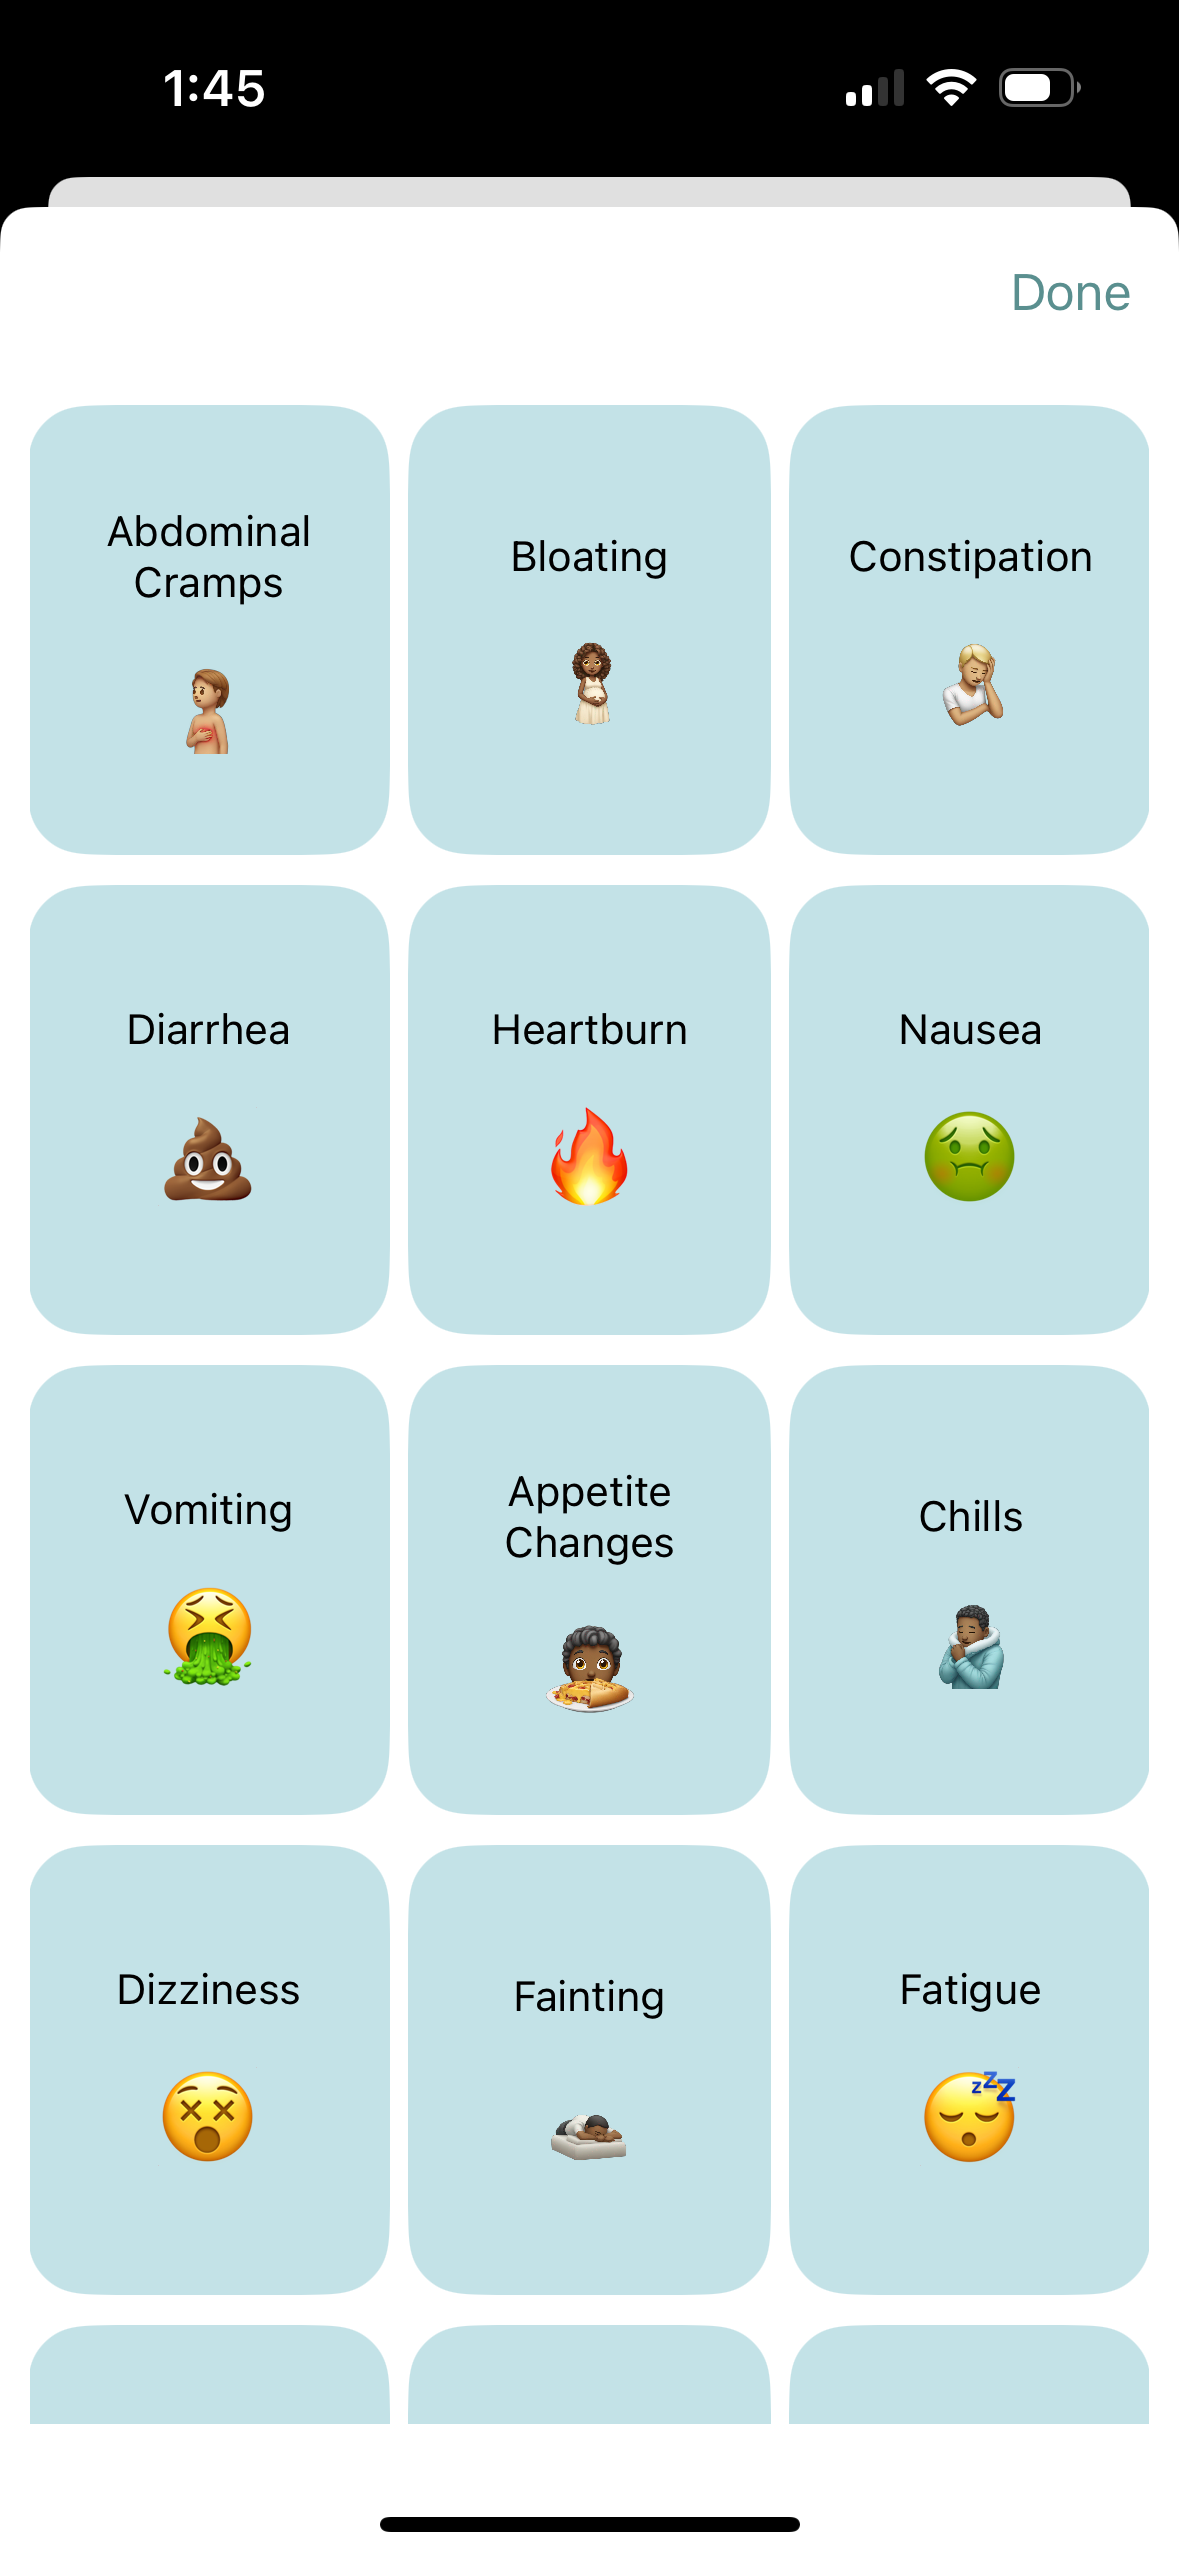
\includegraphics[width=0.25\linewidth]{thesis//chapters//images/uniqueSymptomEmojis.PNG}
    \caption{Unique Emojis for Symptoms}
    \label{fig:enter-label}
\end{figure}

Furthermore, while there currently exists only one generic tree nut emoji, my application necessitated the individual distinction of various tree nuts. To avoid visual monotony, I introduced custom emojis tailored to each specific tree nut. This customization not only enhanced the aesthetic appeal but also improved clarity and user experience.

\begin{figure} [H]
    \centering
    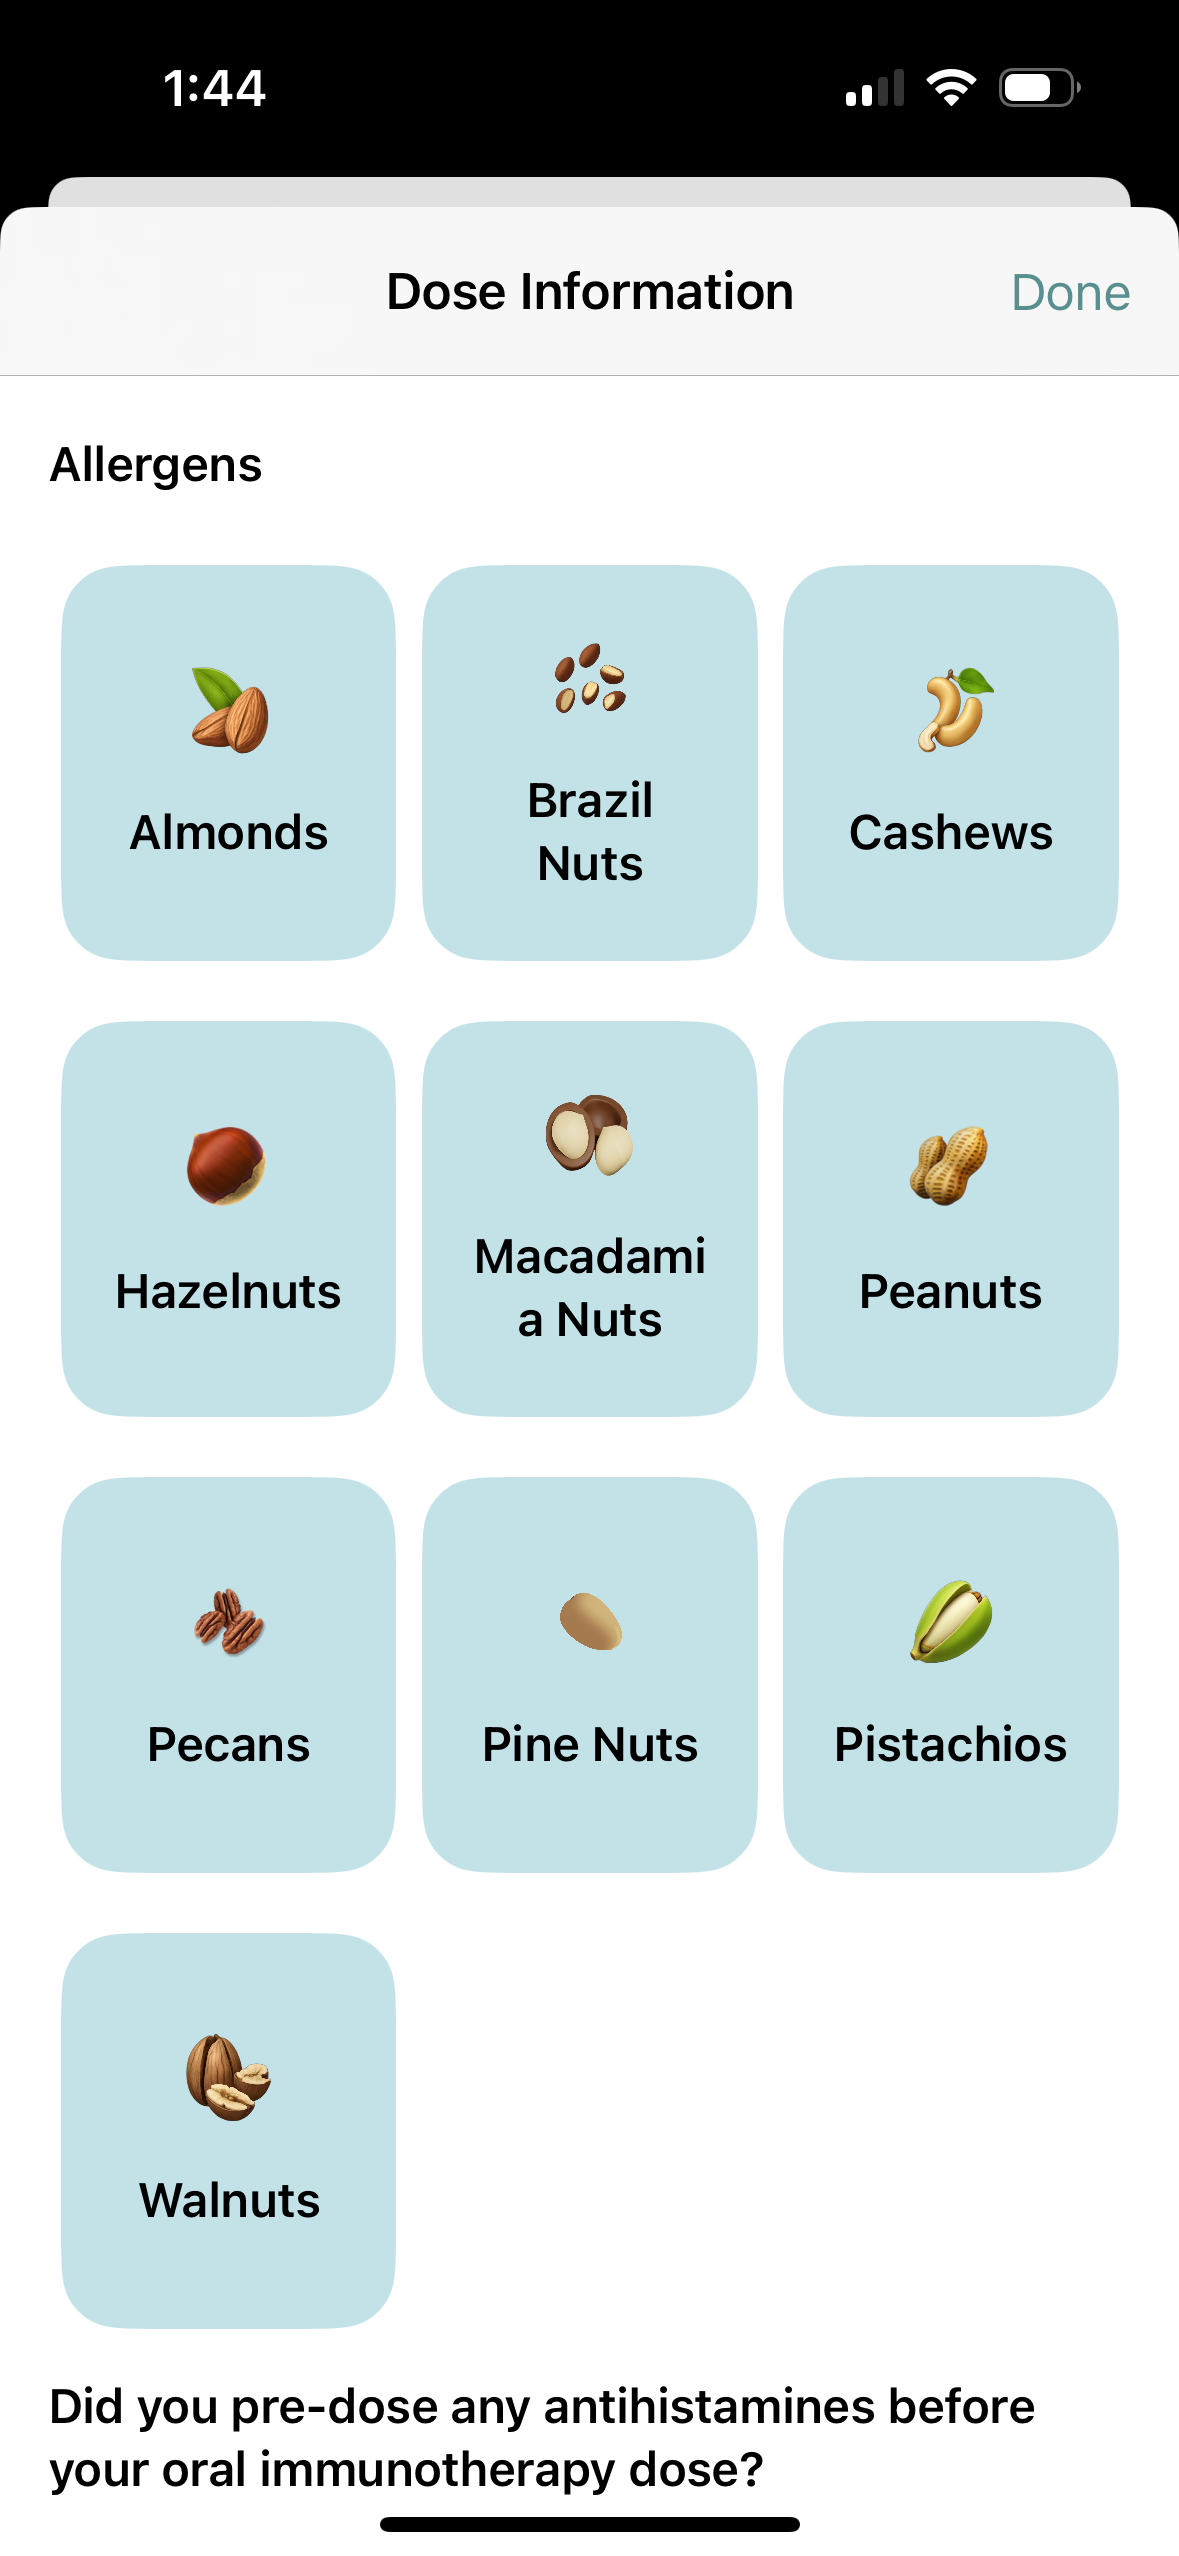
\includegraphics[width=0.25\linewidth]{thesis//chapters//images/uniqueNutEmojis.PNG}
    \caption{Unique Emojis for Nuts}
    \label{fig:enter-label}
\end{figure}

Another enhancement I added to the UI of the application was tips. Utilizing Apple's TipKit, I was able to add helpful pop-ups and messages to the user, explaining how to use different features of the application.

While many of the tips appear as the user is getting set up with the app, I was also able to utilize custom settings, like "displayFrequency" to customize how often new tips are presented after other tips have been displayed. This helped introduce the tips in stages, to not overwhelm the user with too many at once.

\begin{figure} [H]
    \centering
    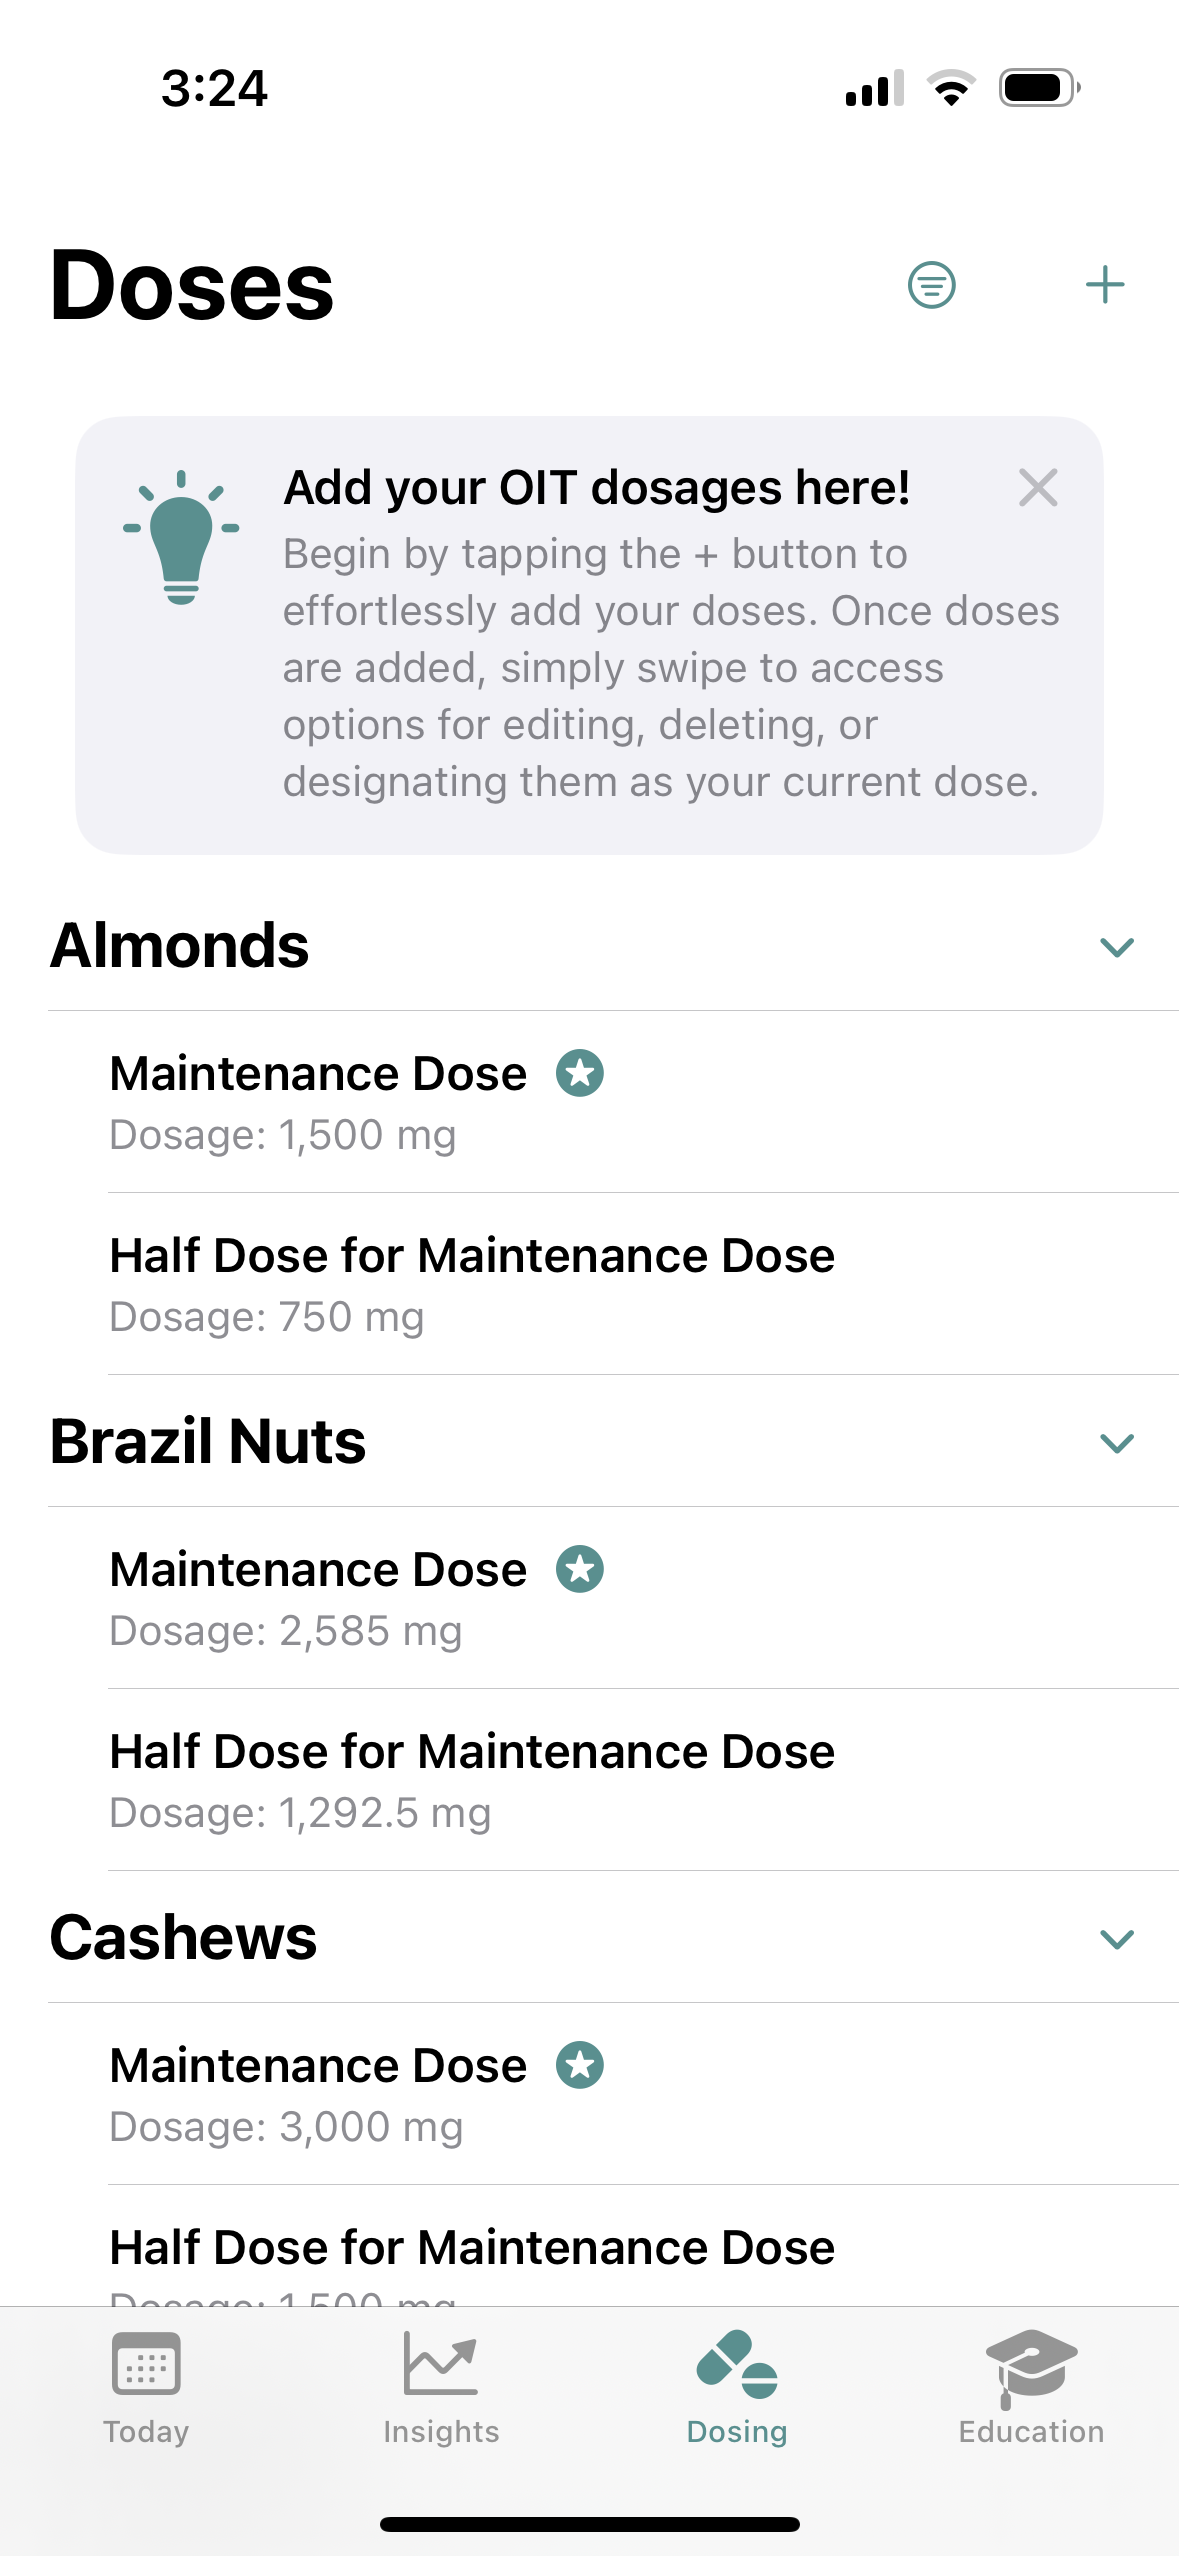
\includegraphics[width=0.2\linewidth]{thesis//chapters//images/dosesTip.PNG}
    \caption{Doses Tab Tip}
    \label{fig:enter-label}
\end{figure}

\subsection{Additional Resources}

As mentioned in Section \ref{section:consultingImmunologists}: Consultation with Immunologists, many immunologists advised incorporating some type of feature to allow users to upload images of their emergency action plans to the Resources tab. So, I added an "Important Documents" section to the Resources tab to allow patients to keep all of their important documents (e.g. Emergency Action Plan) in one place so that they can find them easily.

Users can easily tap on the "Select Images" button to add more documents, tap on documents in the section to view them, and tap on the "x" buttons below the images to remove them as needed.

\begin{figure} [H]
    \centering
    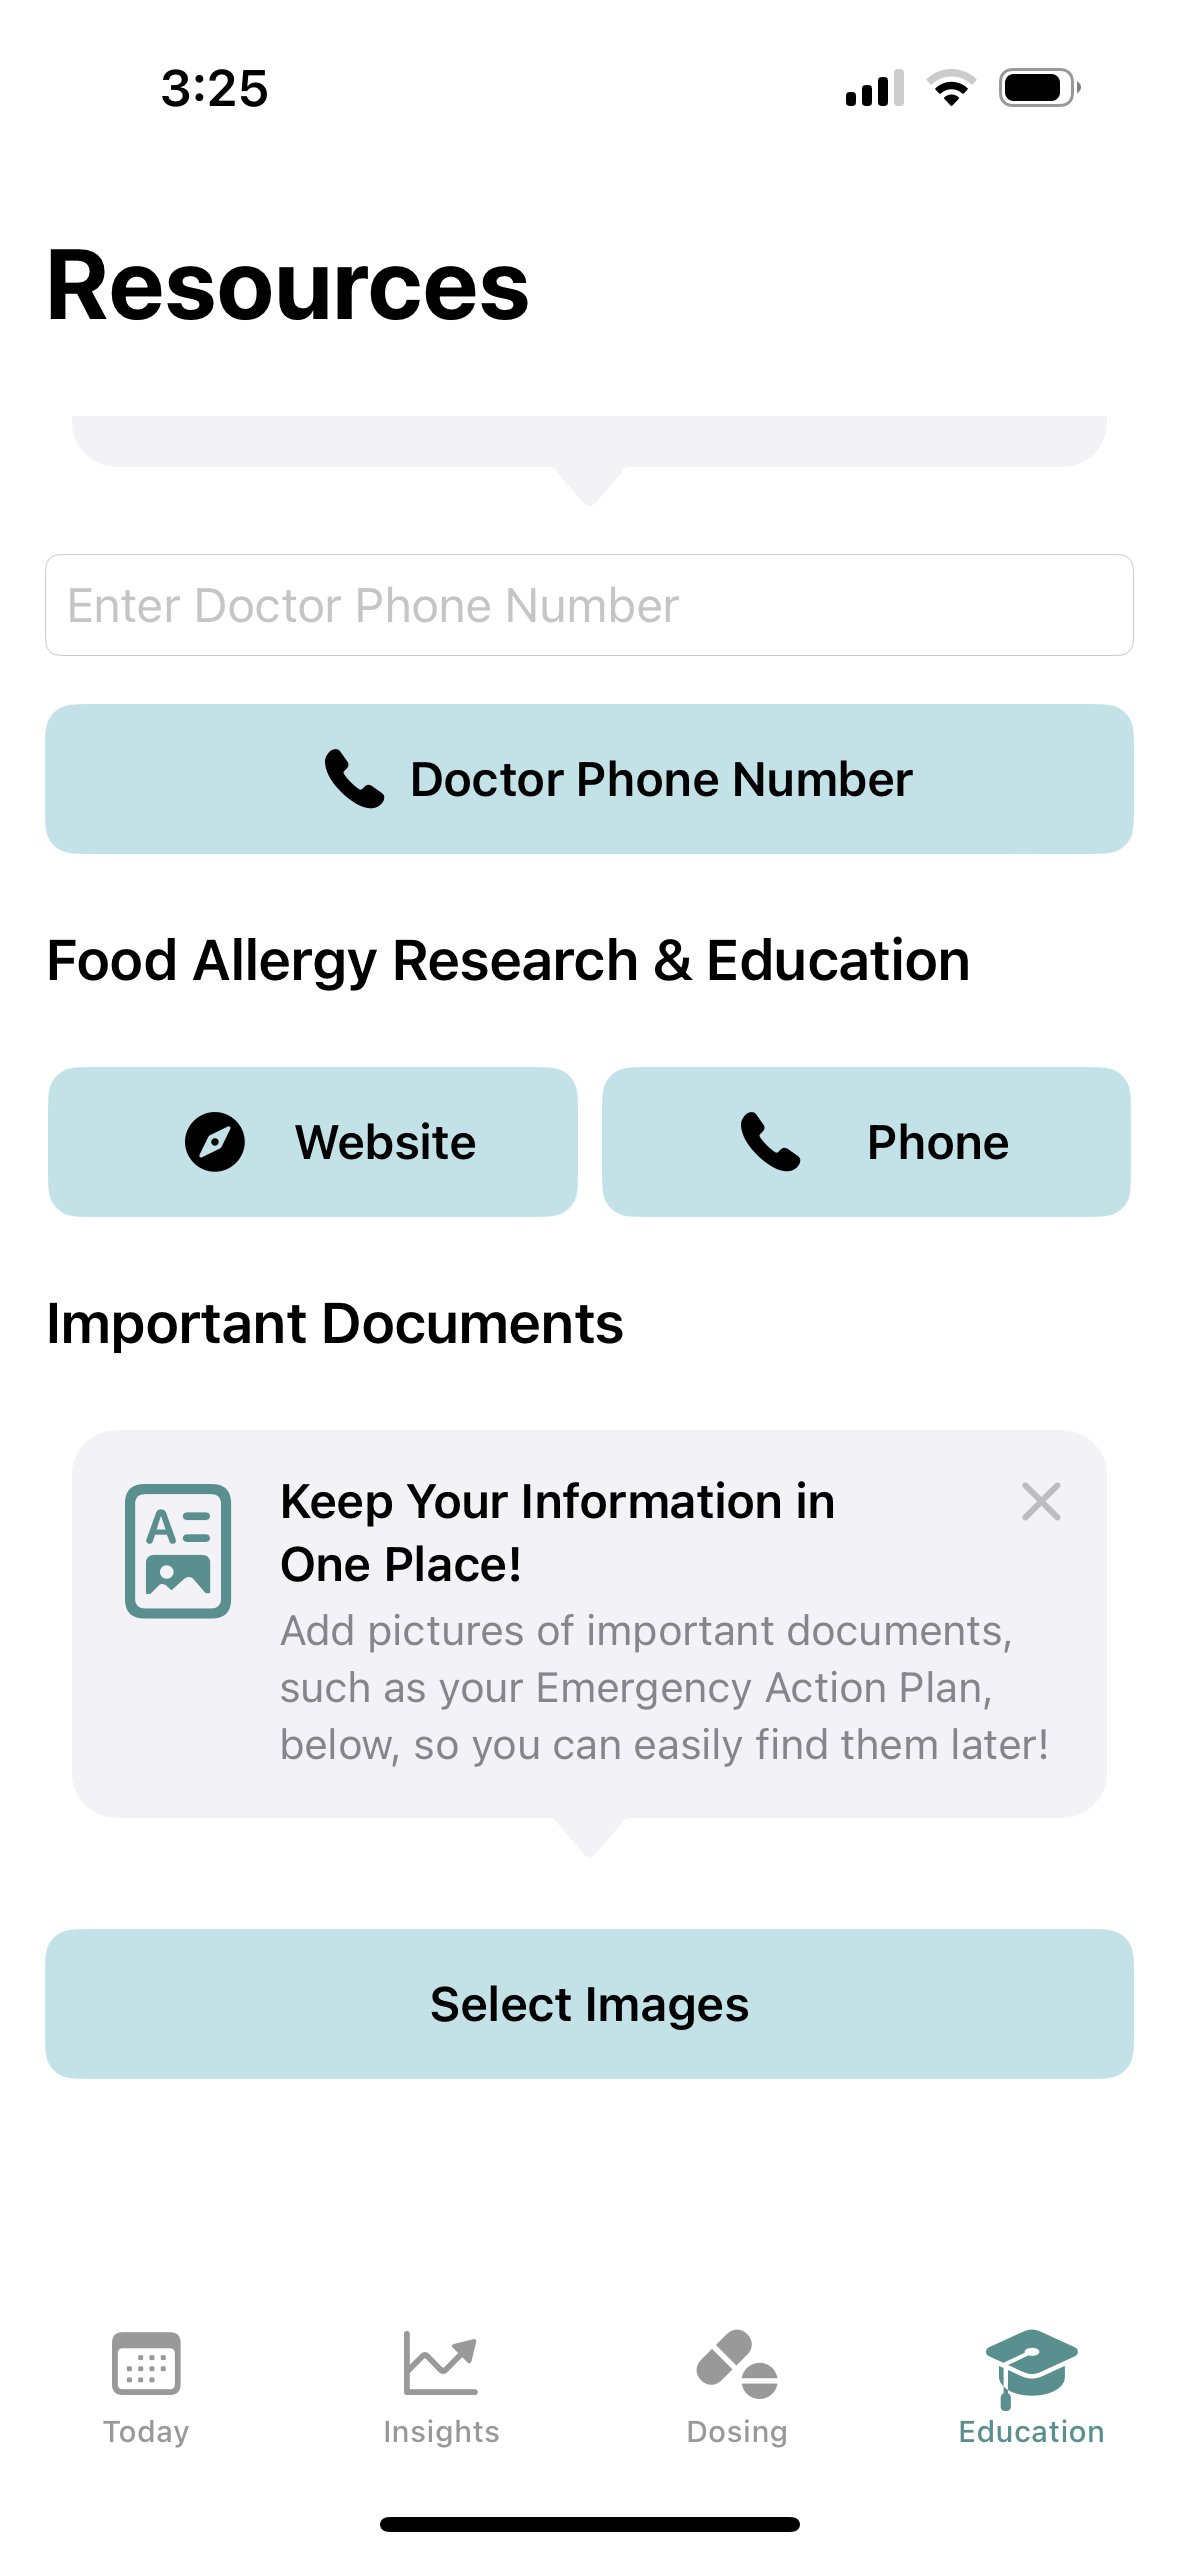
\includegraphics[width=0.25\linewidth]{thesis//chapters//images/importantDocs.PNG}
    \caption{Important Documents Section}
    \label{fig:enter-label}
\end{figure}

\begin{figure} [H]
    \centering
    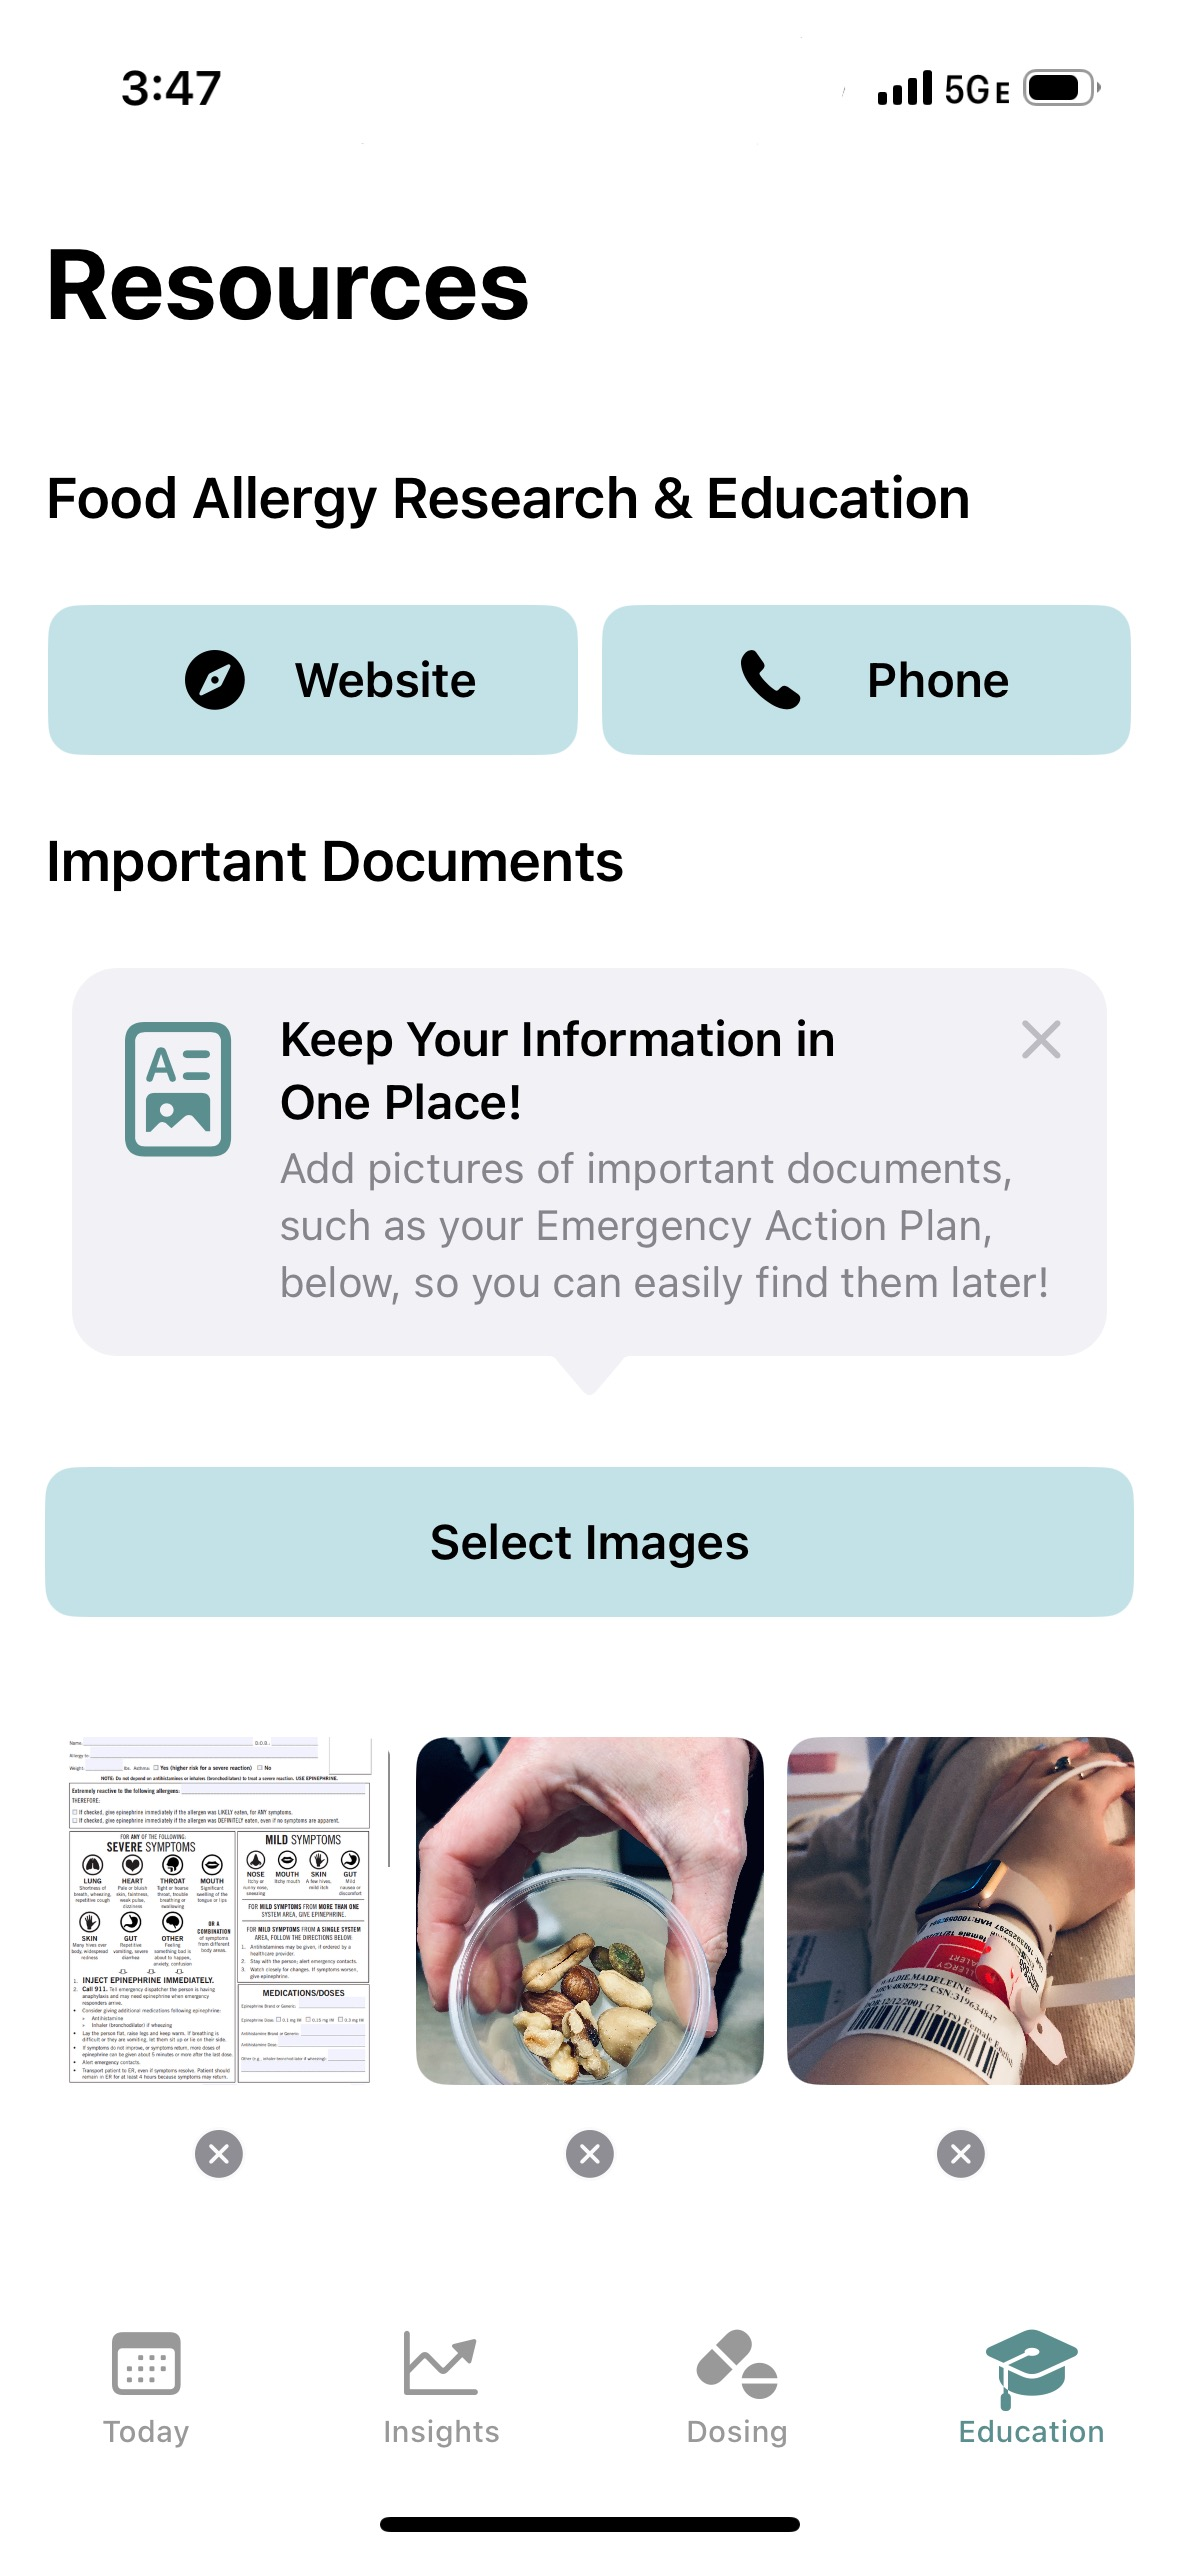
\includegraphics[width=0.25\linewidth]{thesis//chapters//images/importantDocs2.jpg}
    \caption{Important Documents Section With Documents Added}
    \label{fig:enter-label}
\end{figure}

\begin{figure} [H]
    \centering
    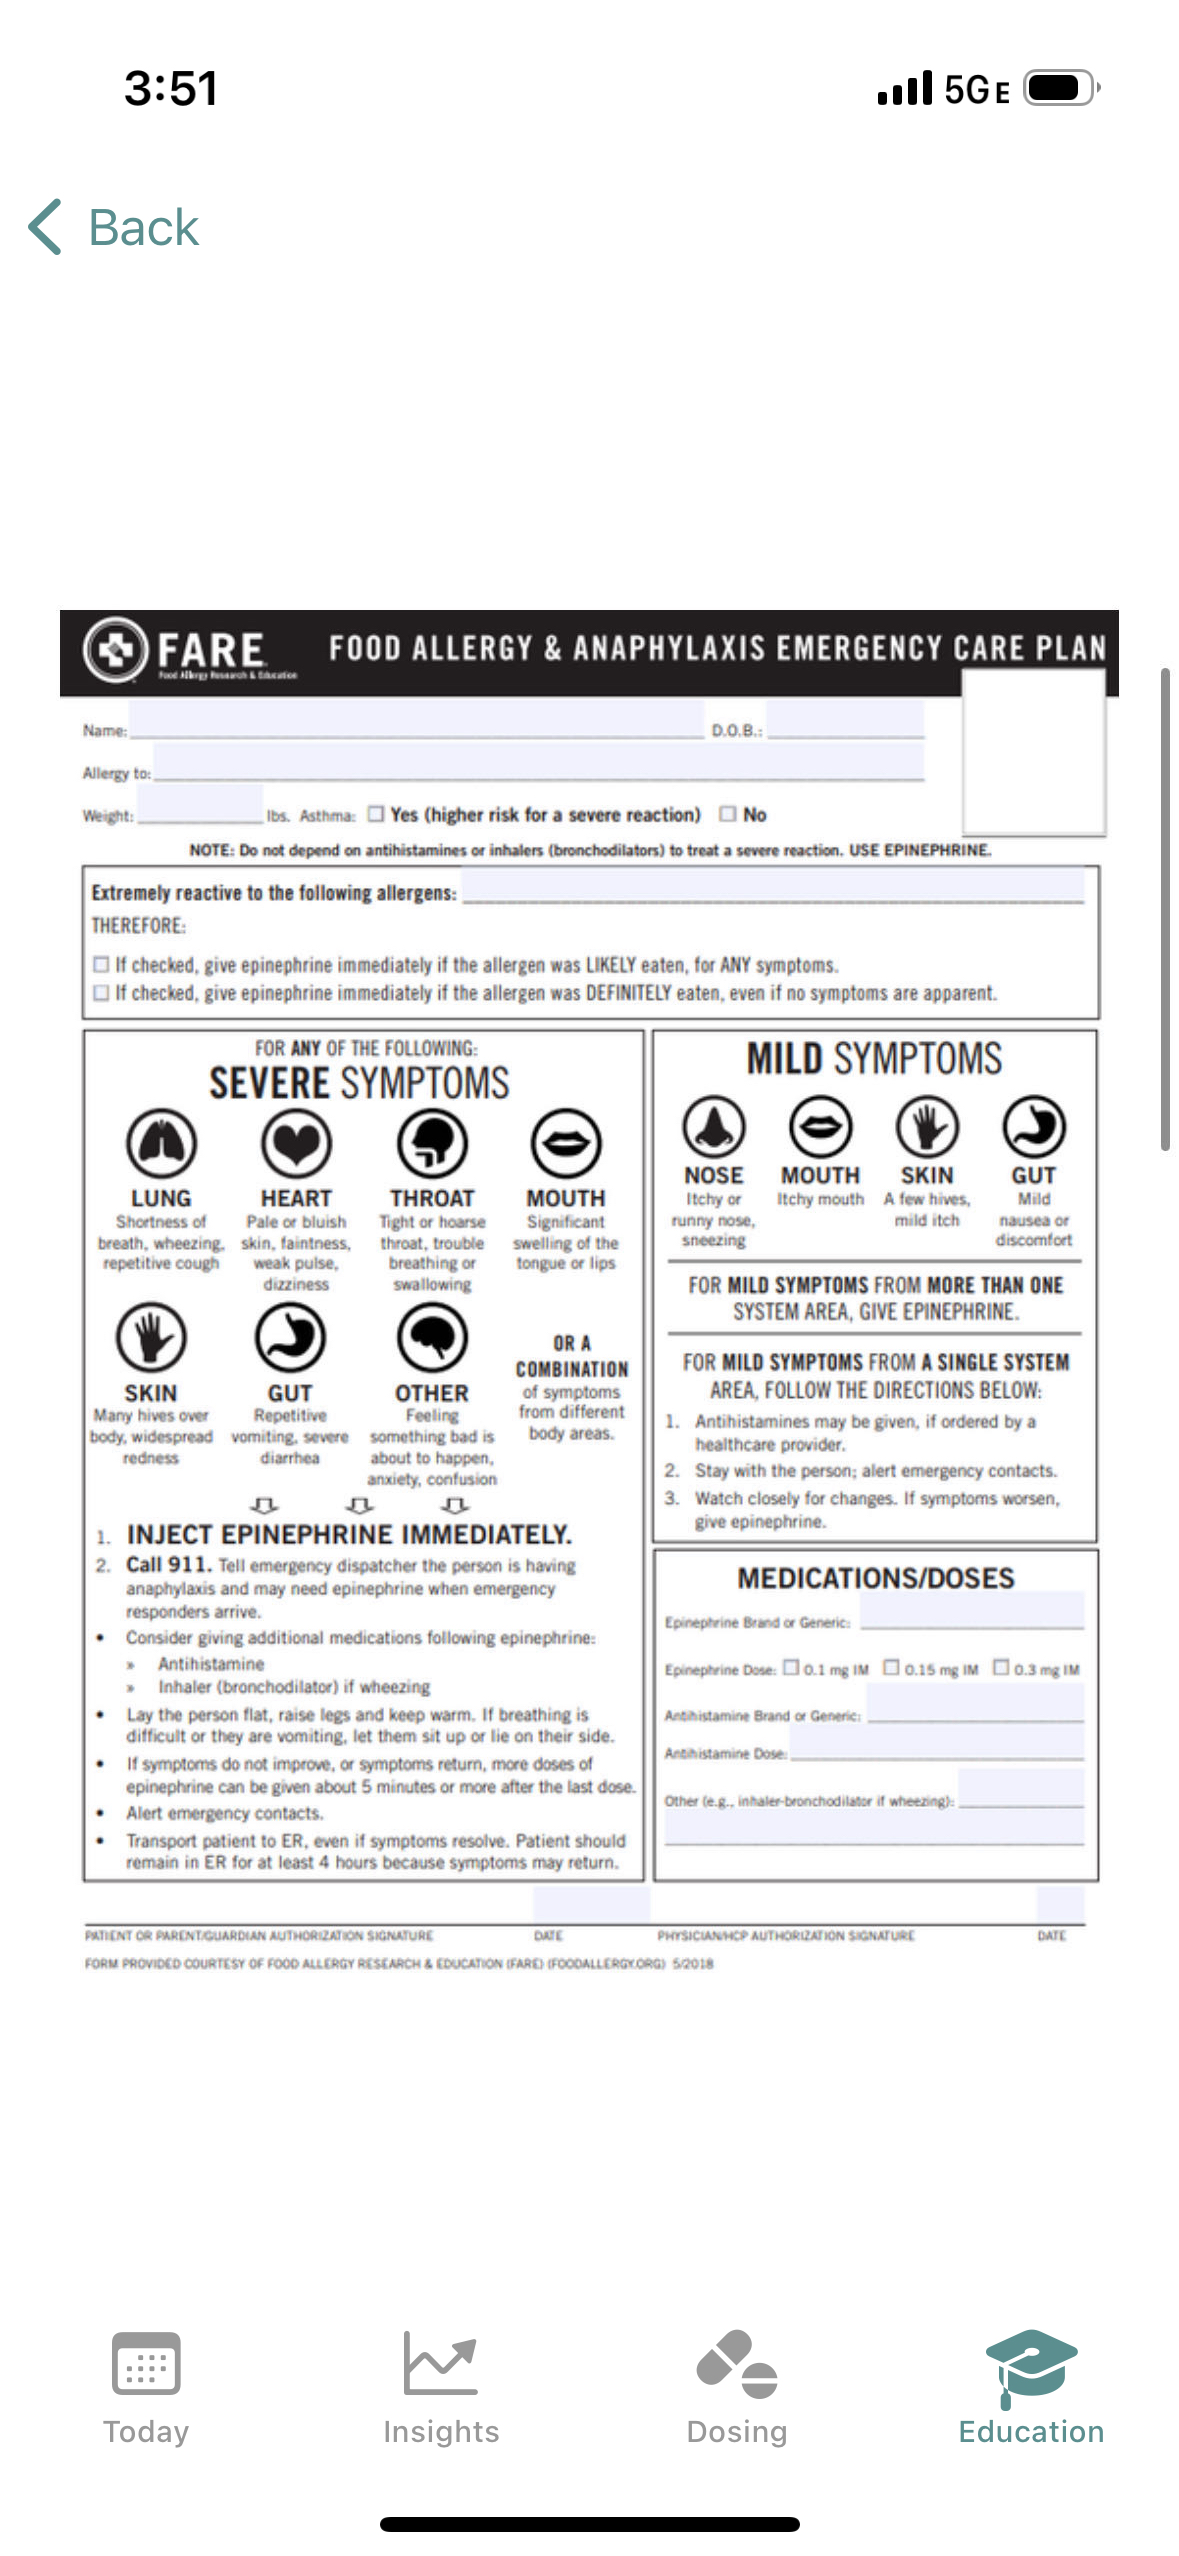
\includegraphics[width=0.25\linewidth]{thesis//chapters//images/importantDocs3.jpg}
    \caption{Tapping to View Important Document}
    \label{fig:enter-label}
\end{figure}

Additionally, I added a section for users to add their doctor's phone number, so they can easily reach out to them if needed.

\begin{figure} [H]
    \centering
    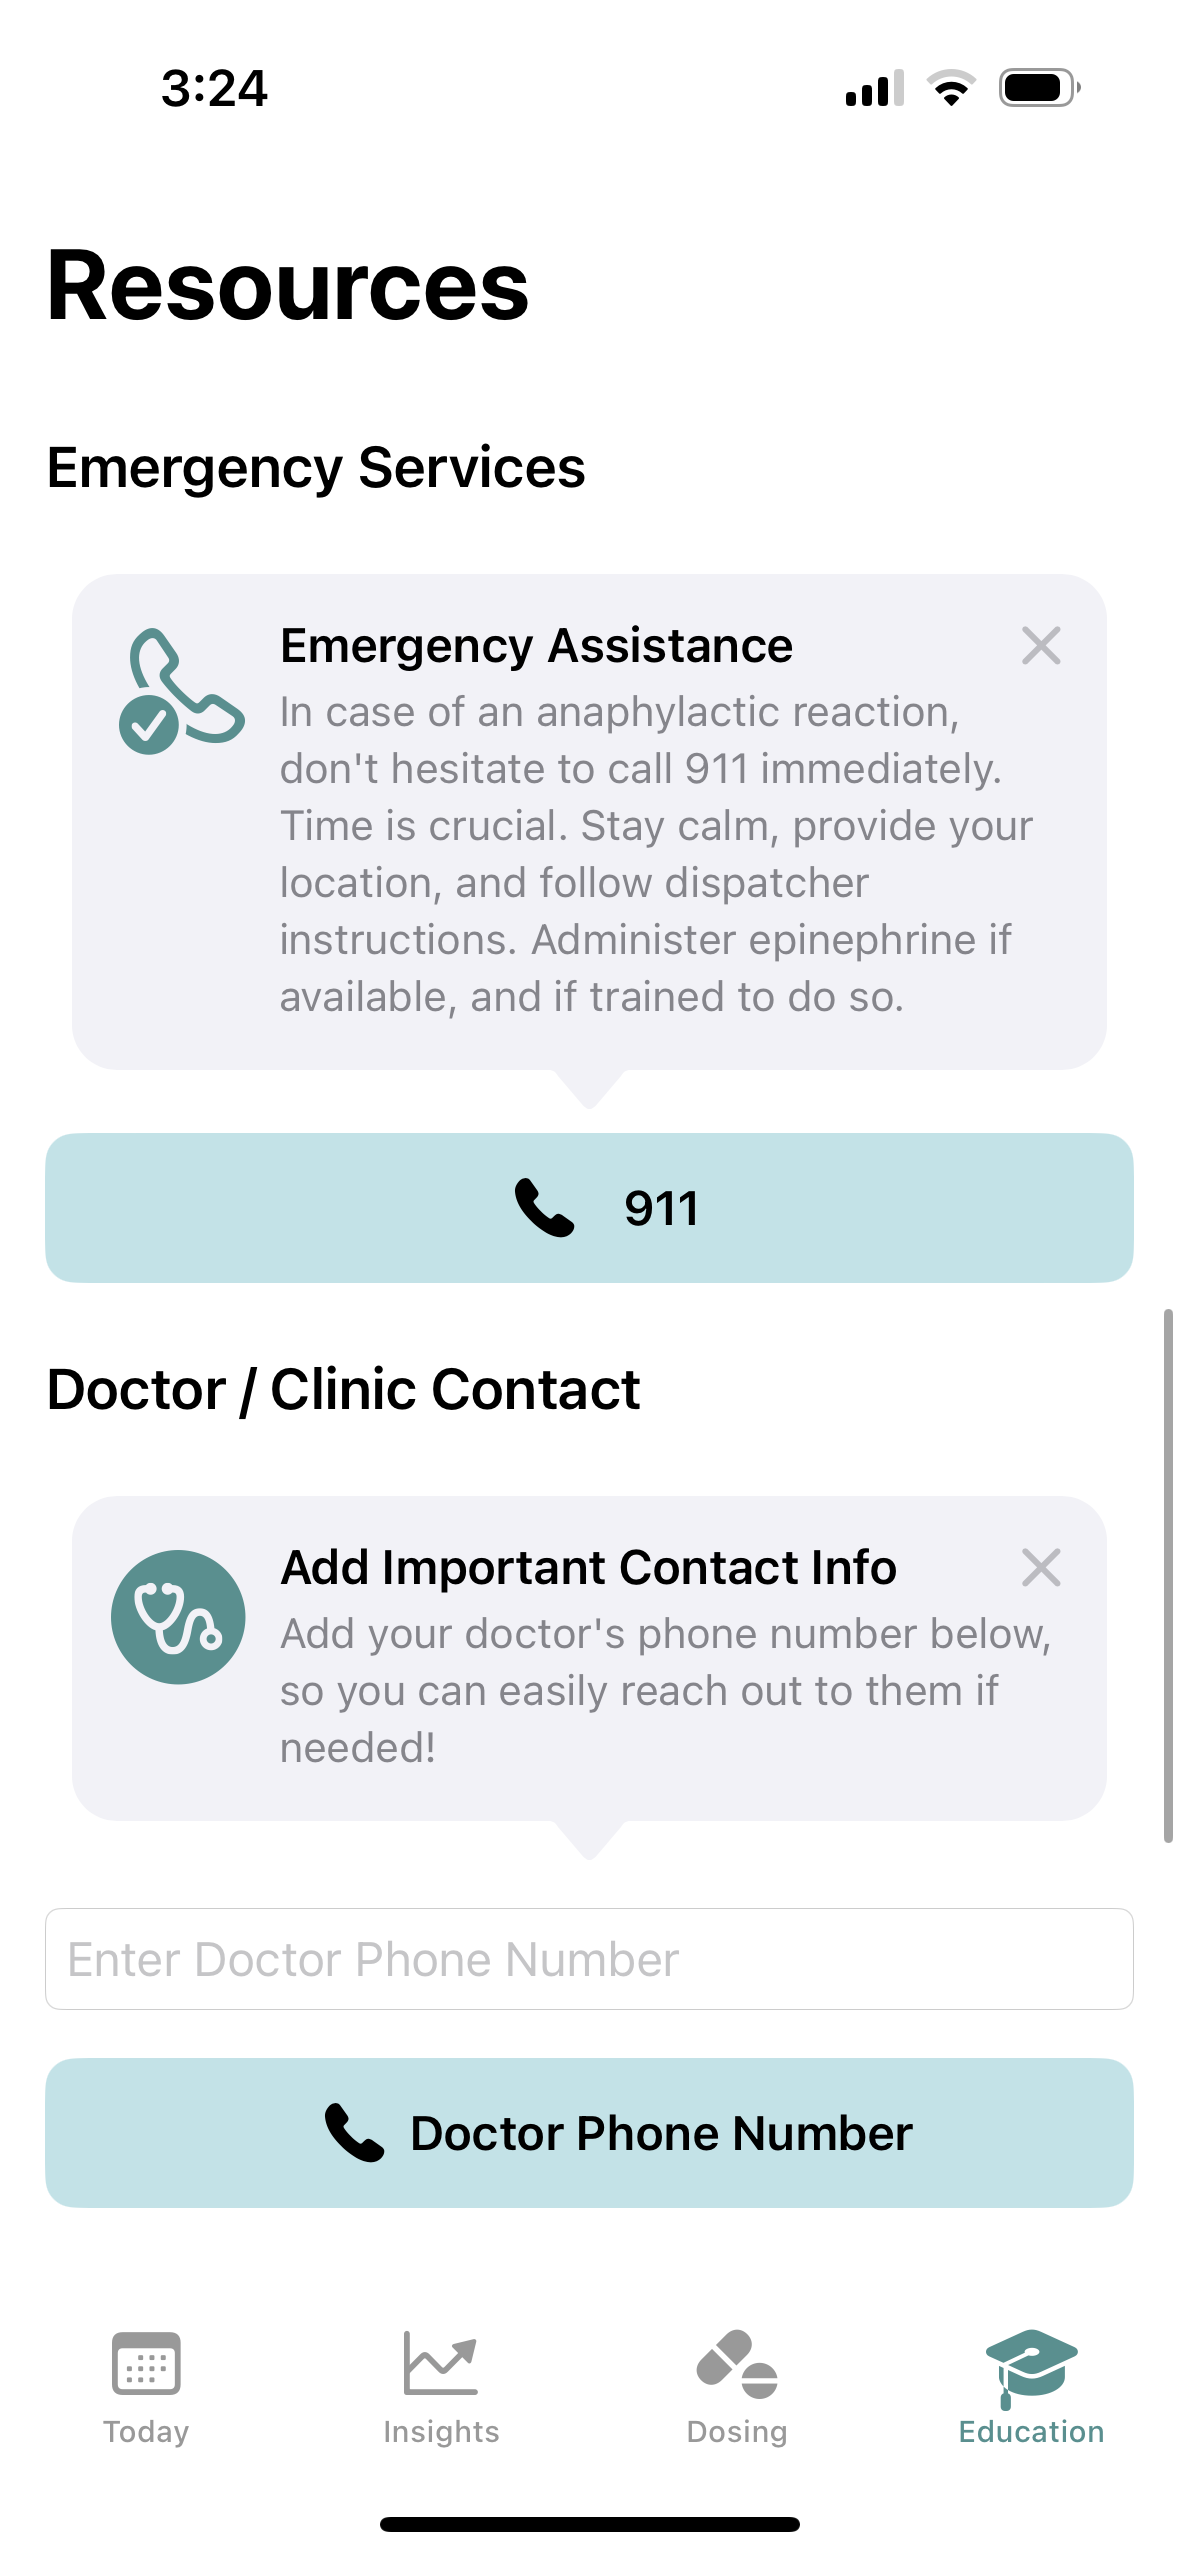
\includegraphics[width=0.25\linewidth]{thesis//chapters//images/doctorContact.PNG}
    \caption{Doctor / Clinic Contact Info Section}
    \label{fig:enter-label}
\end{figure}

\subsection{Profile}

While the profile section remained mostly the same as the prototypes, I added a few subtle changes. First, I added a section to add a profile picture. I thought this added a needed element of personalization to the app and tied together the personal information section of the profile nicely.

\begin{figure} [H]
    \centering
    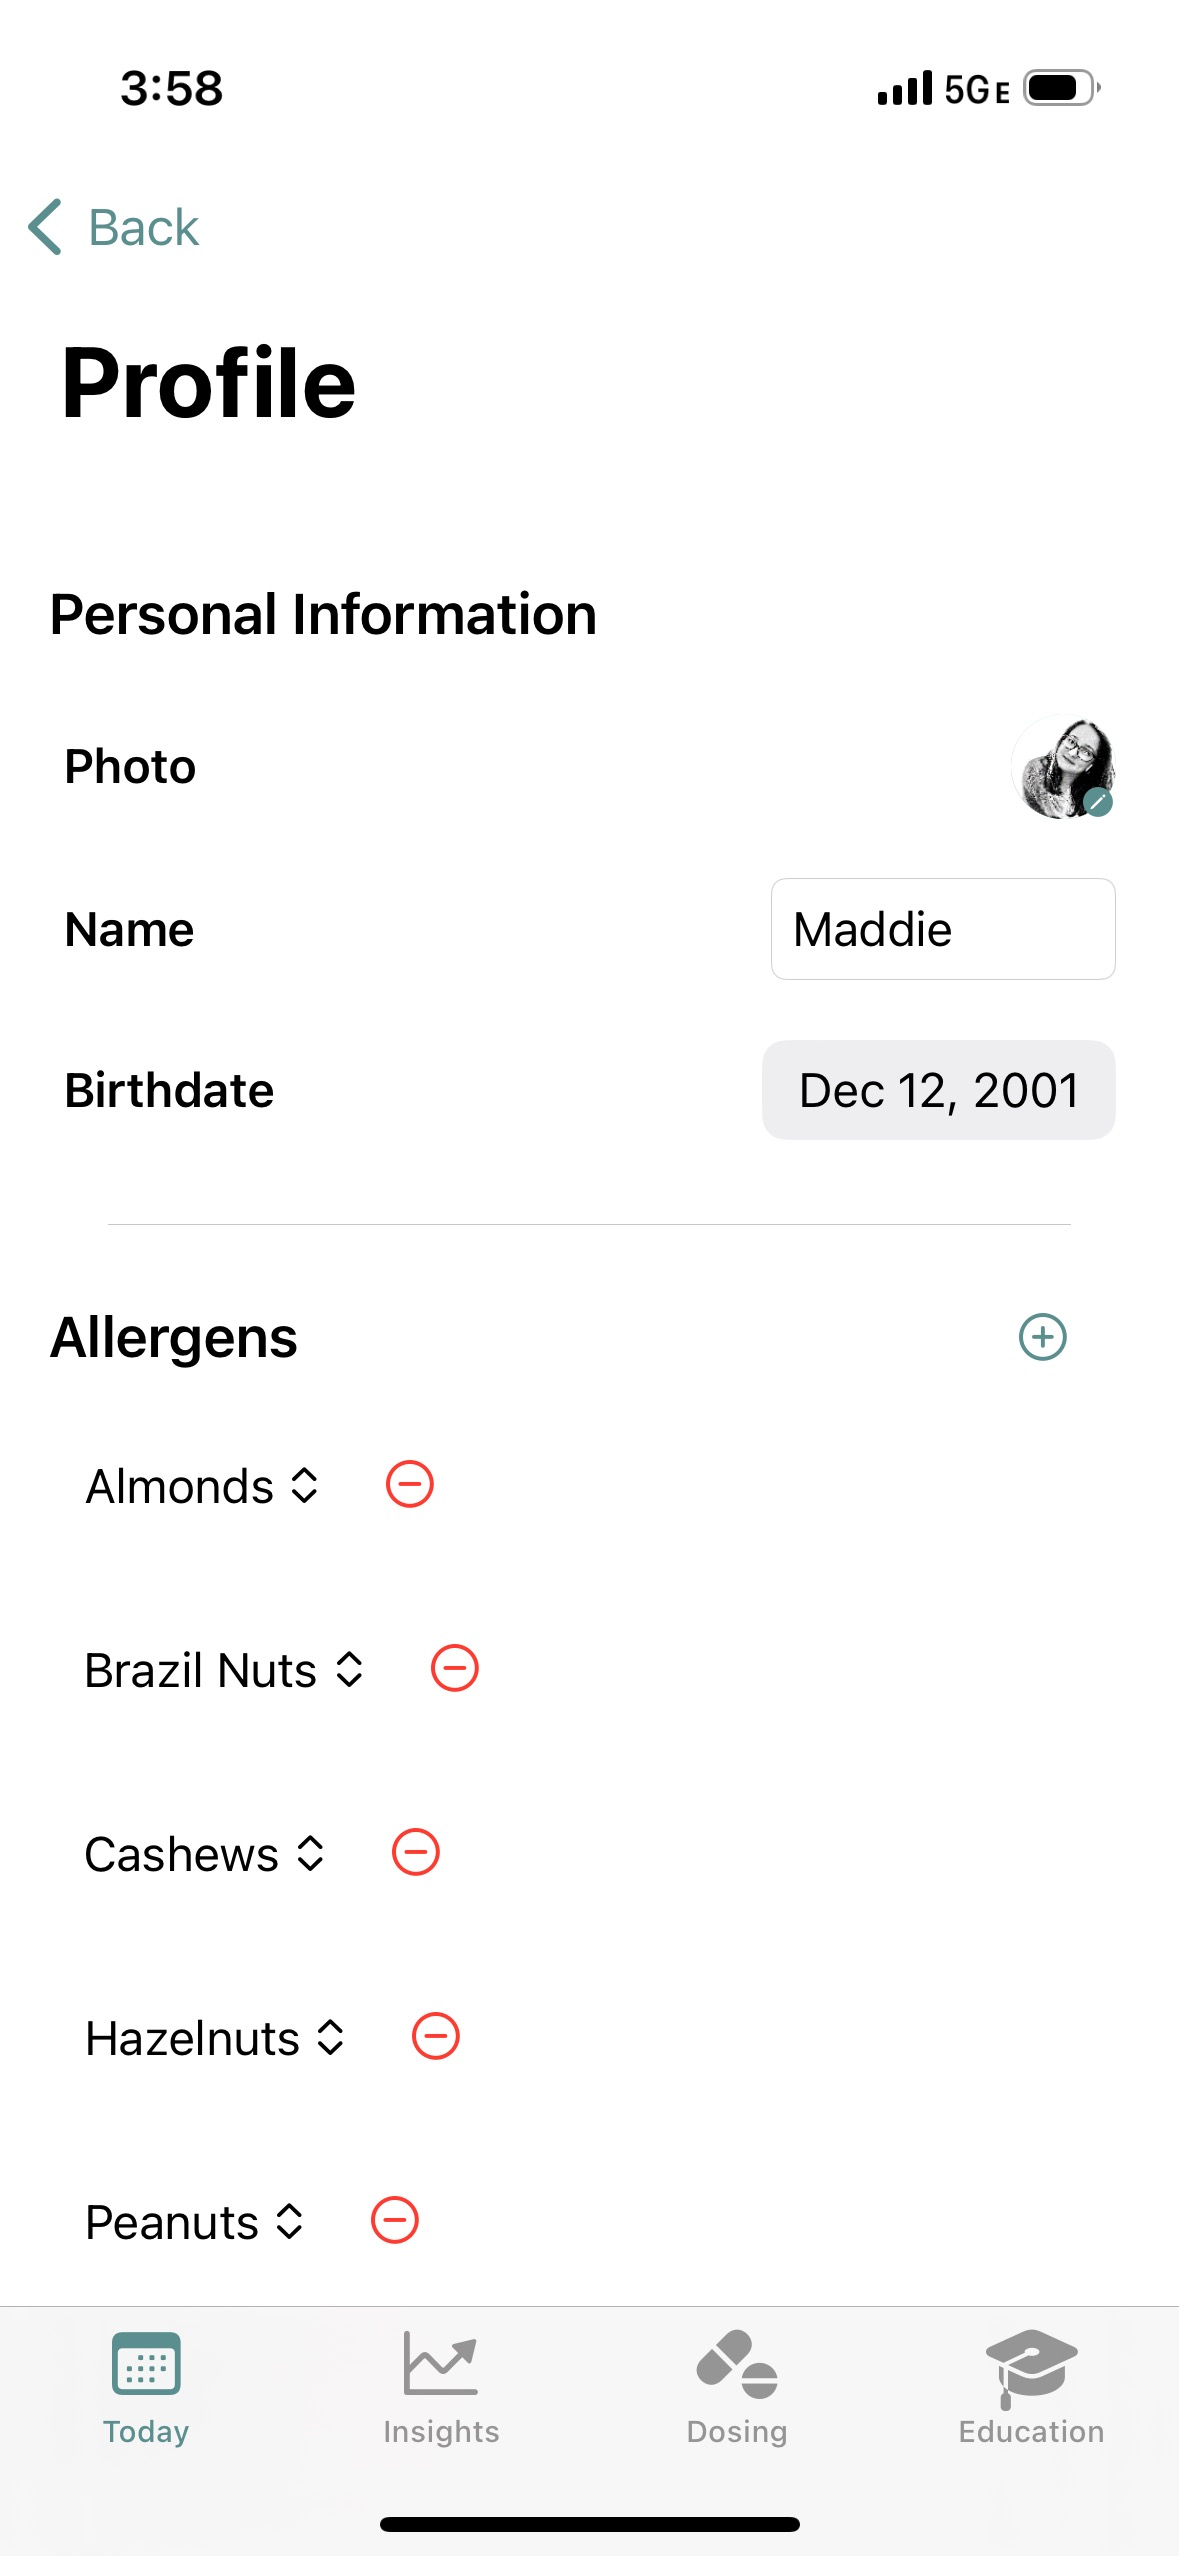
\includegraphics[width=0.25\linewidth]{thesis//chapters//images/profilePic1.jpg}
    \caption{Add Profile Photo Section}
    \label{fig:enter-label}
\end{figure}

\begin{figure} [H]
    \centering
    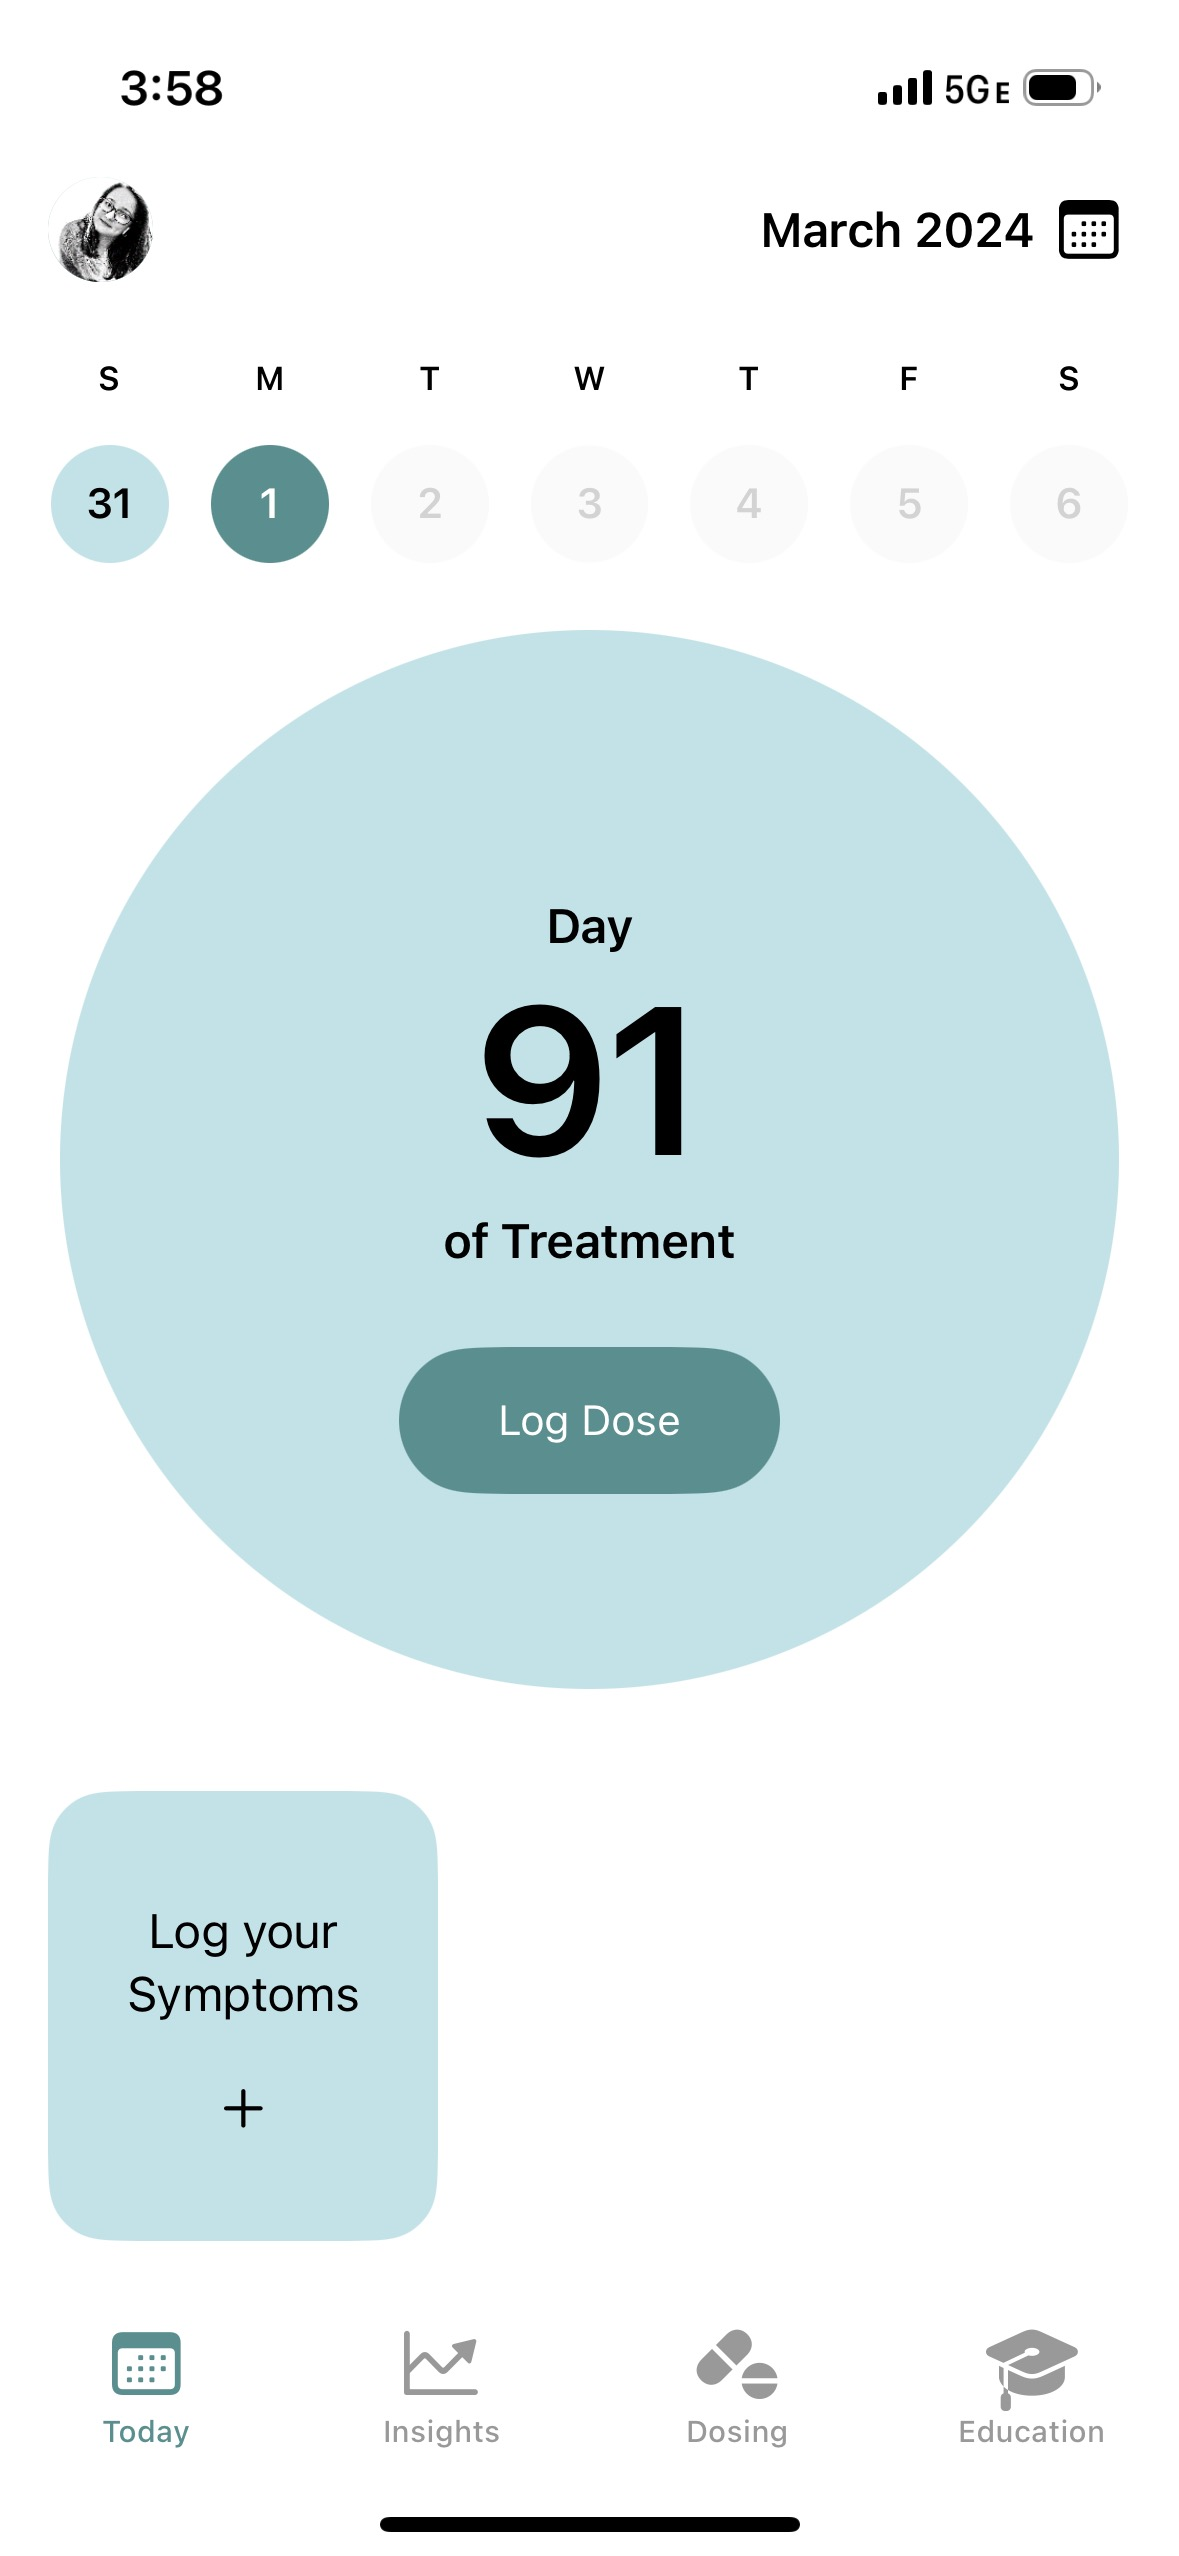
\includegraphics[width=0.25\linewidth]{thesis//chapters//images/profilePic2.jpg}
    \caption{Profile Picture in Top Corner of App}
    \label{fig:enter-label}
\end{figure}

Additionally, when handling users with less common allergens that weren't in the list of common allergens, I ran into issues with no emoji associated with the allergen, as well as issues with the data persistence. To fix this, I added a pop-up when the user selected "Other" from the list of allergens in their profile. This allowed them to enter their allergen's name, as well as an emoji that correlated to that allergen.

\begin{figure} [H]
    \centering
    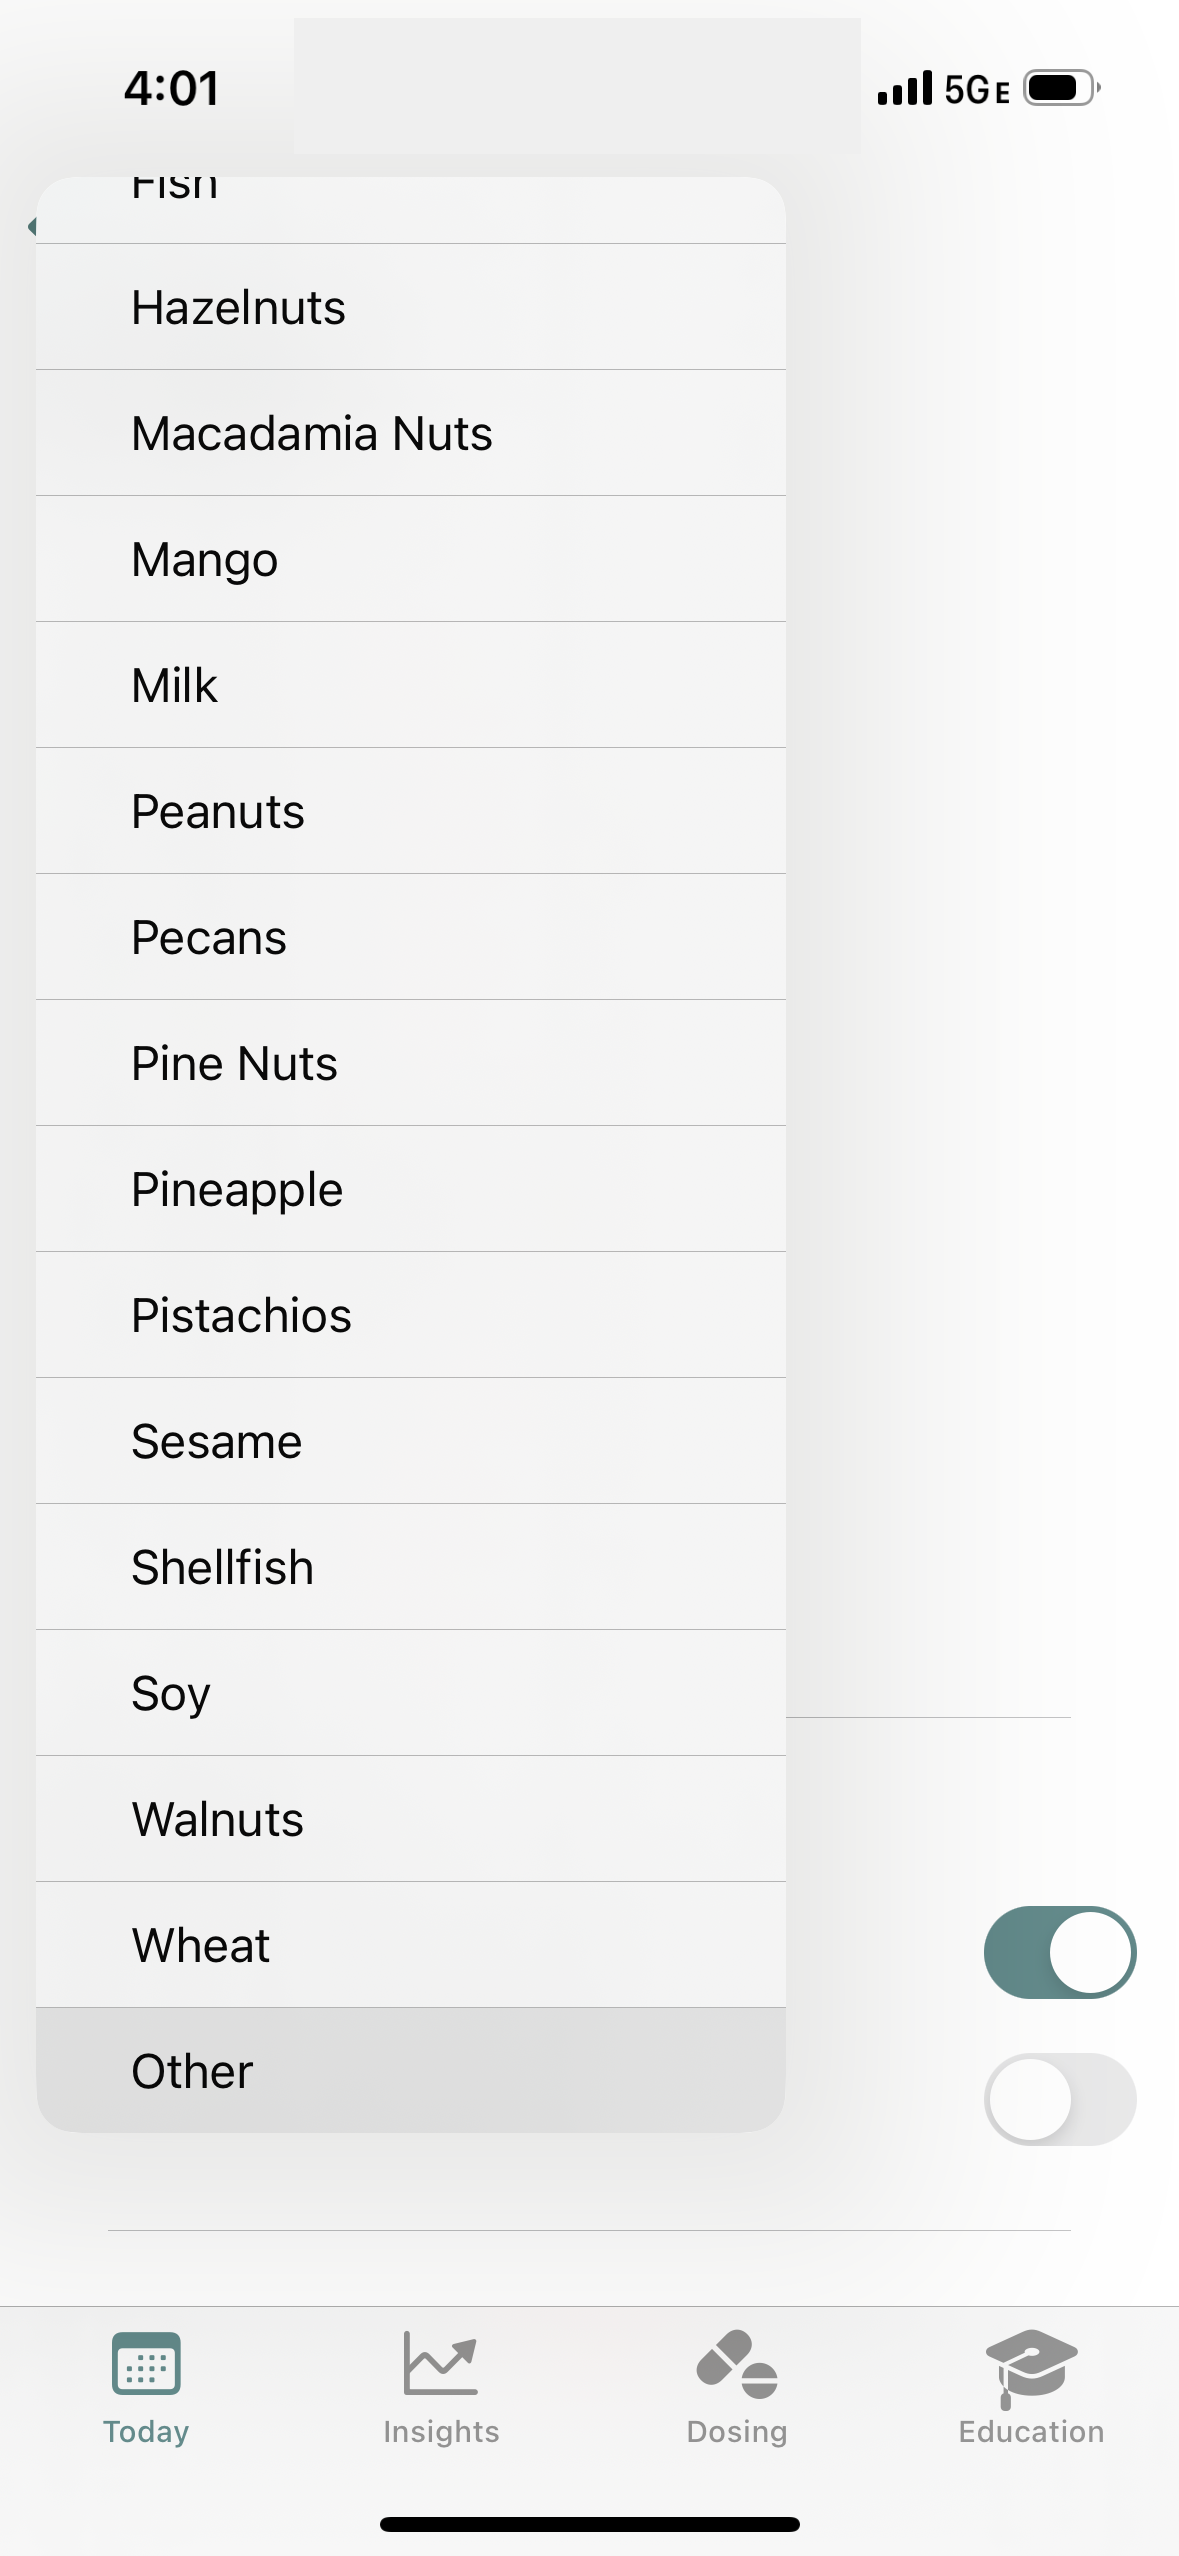
\includegraphics[width=0.25\linewidth]{thesis//chapters//images/otherAllergen1.PNG}
    \caption{User Tapping Other Allergen from Common Allergens List}
    \label{fig:enter-label}
\end{figure}

\begin{figure} [H]
    \centering
    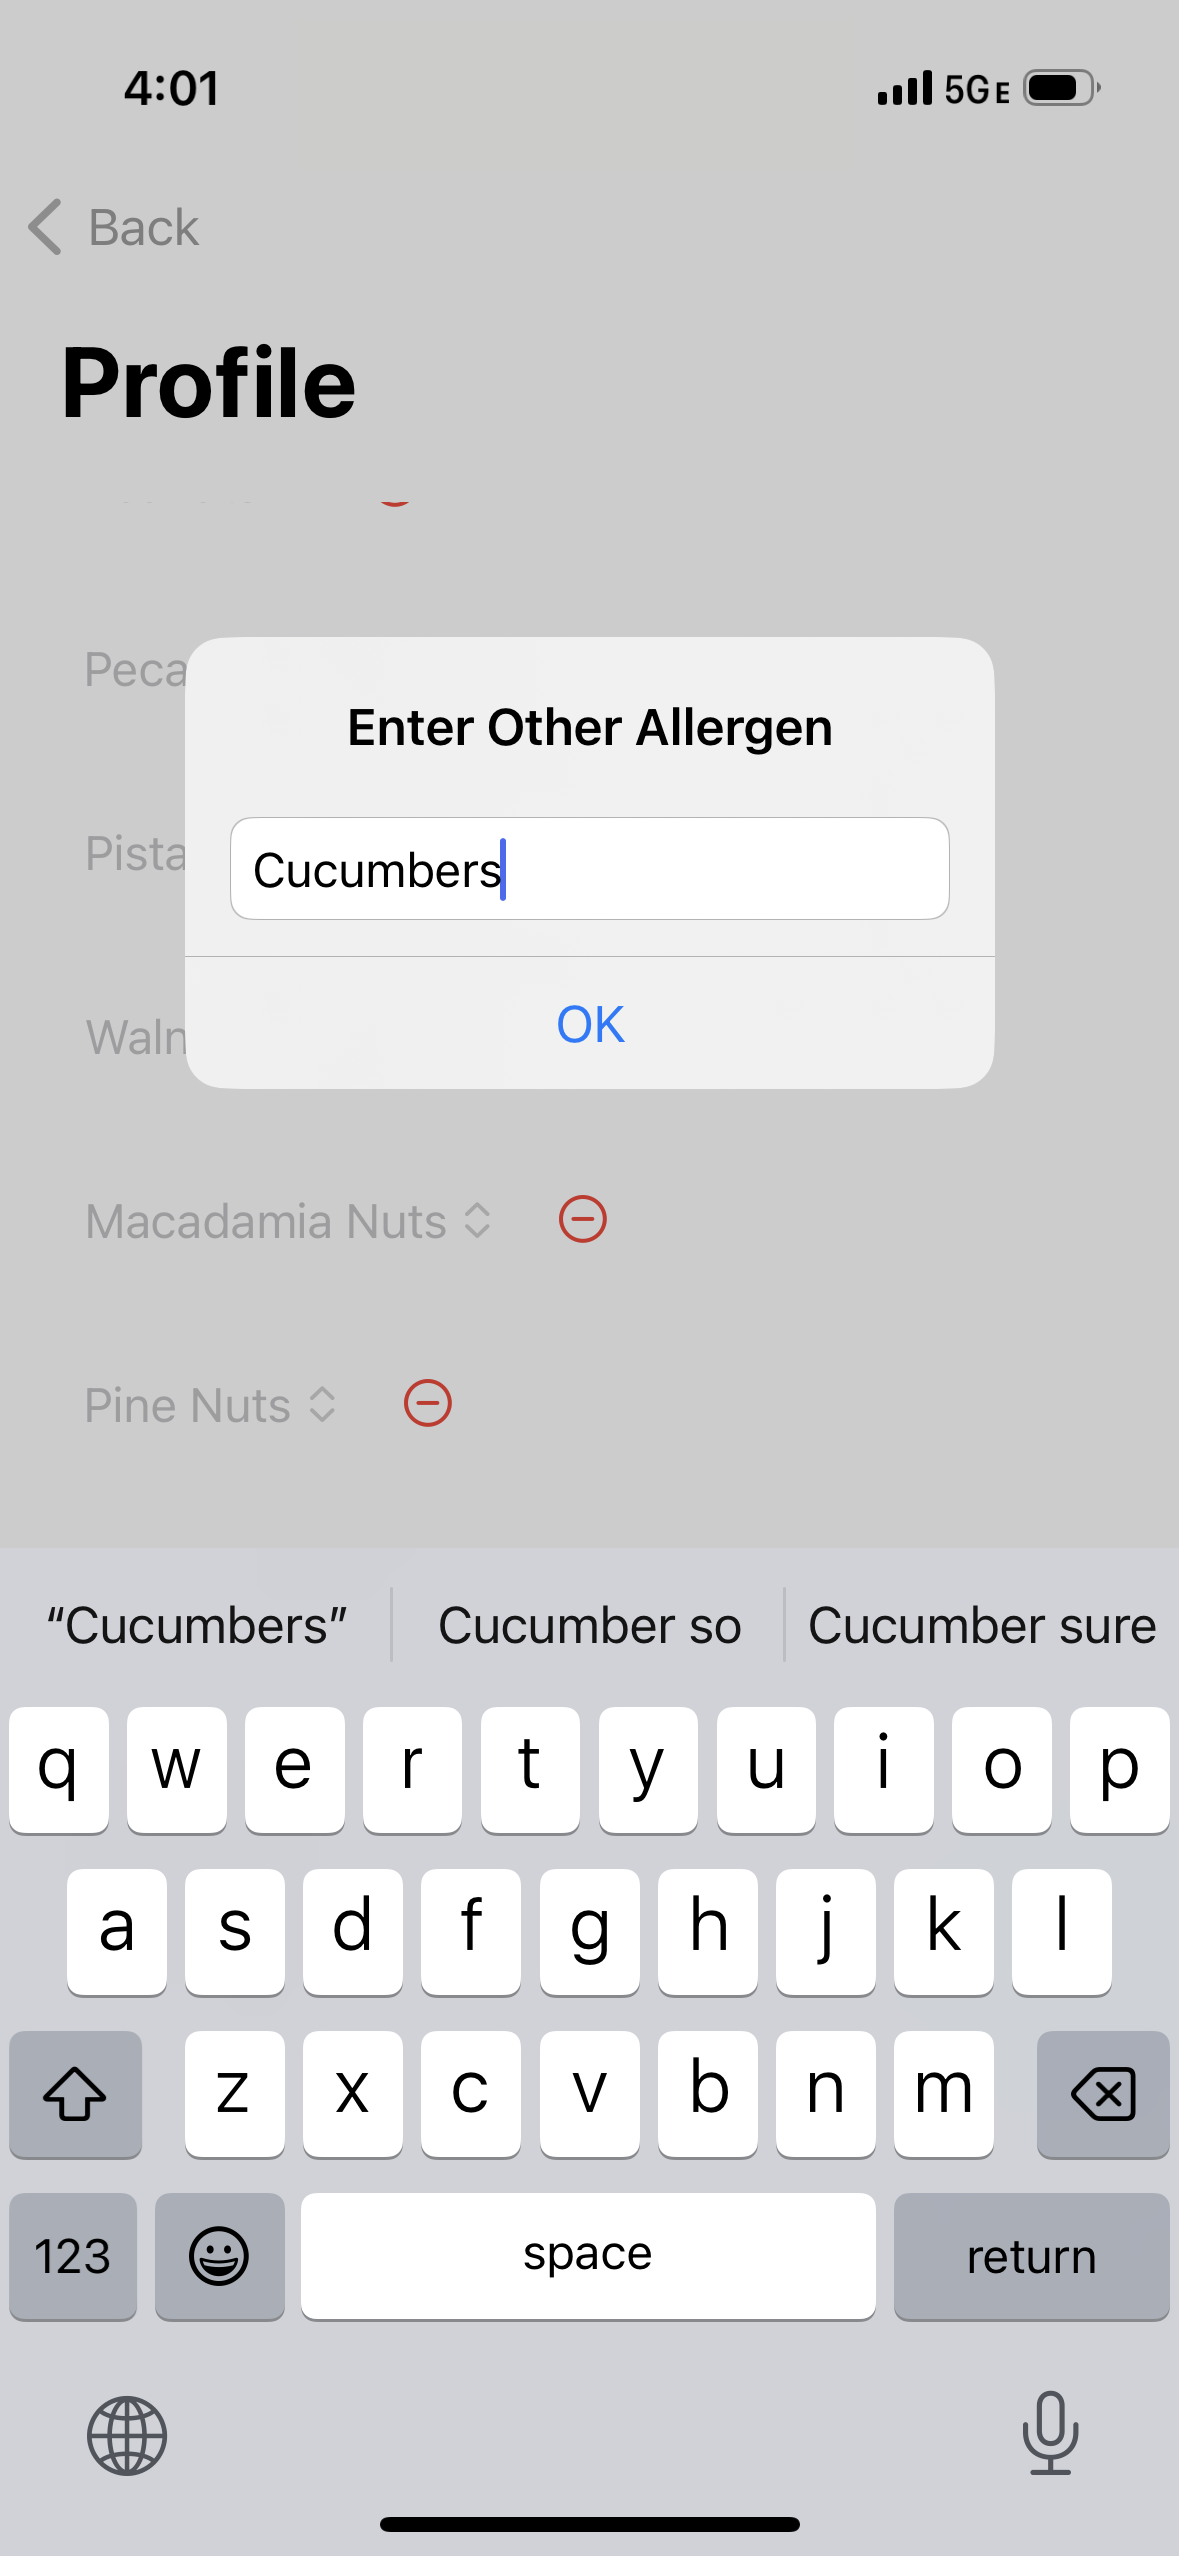
\includegraphics[width=0.25\linewidth]{thesis//chapters//images/otherAllergen3.PNG}
    \caption{User Adding Other Allergen Name}
    \label{fig:enter-label}
\end{figure}

\begin{figure} [H]
    \centering
    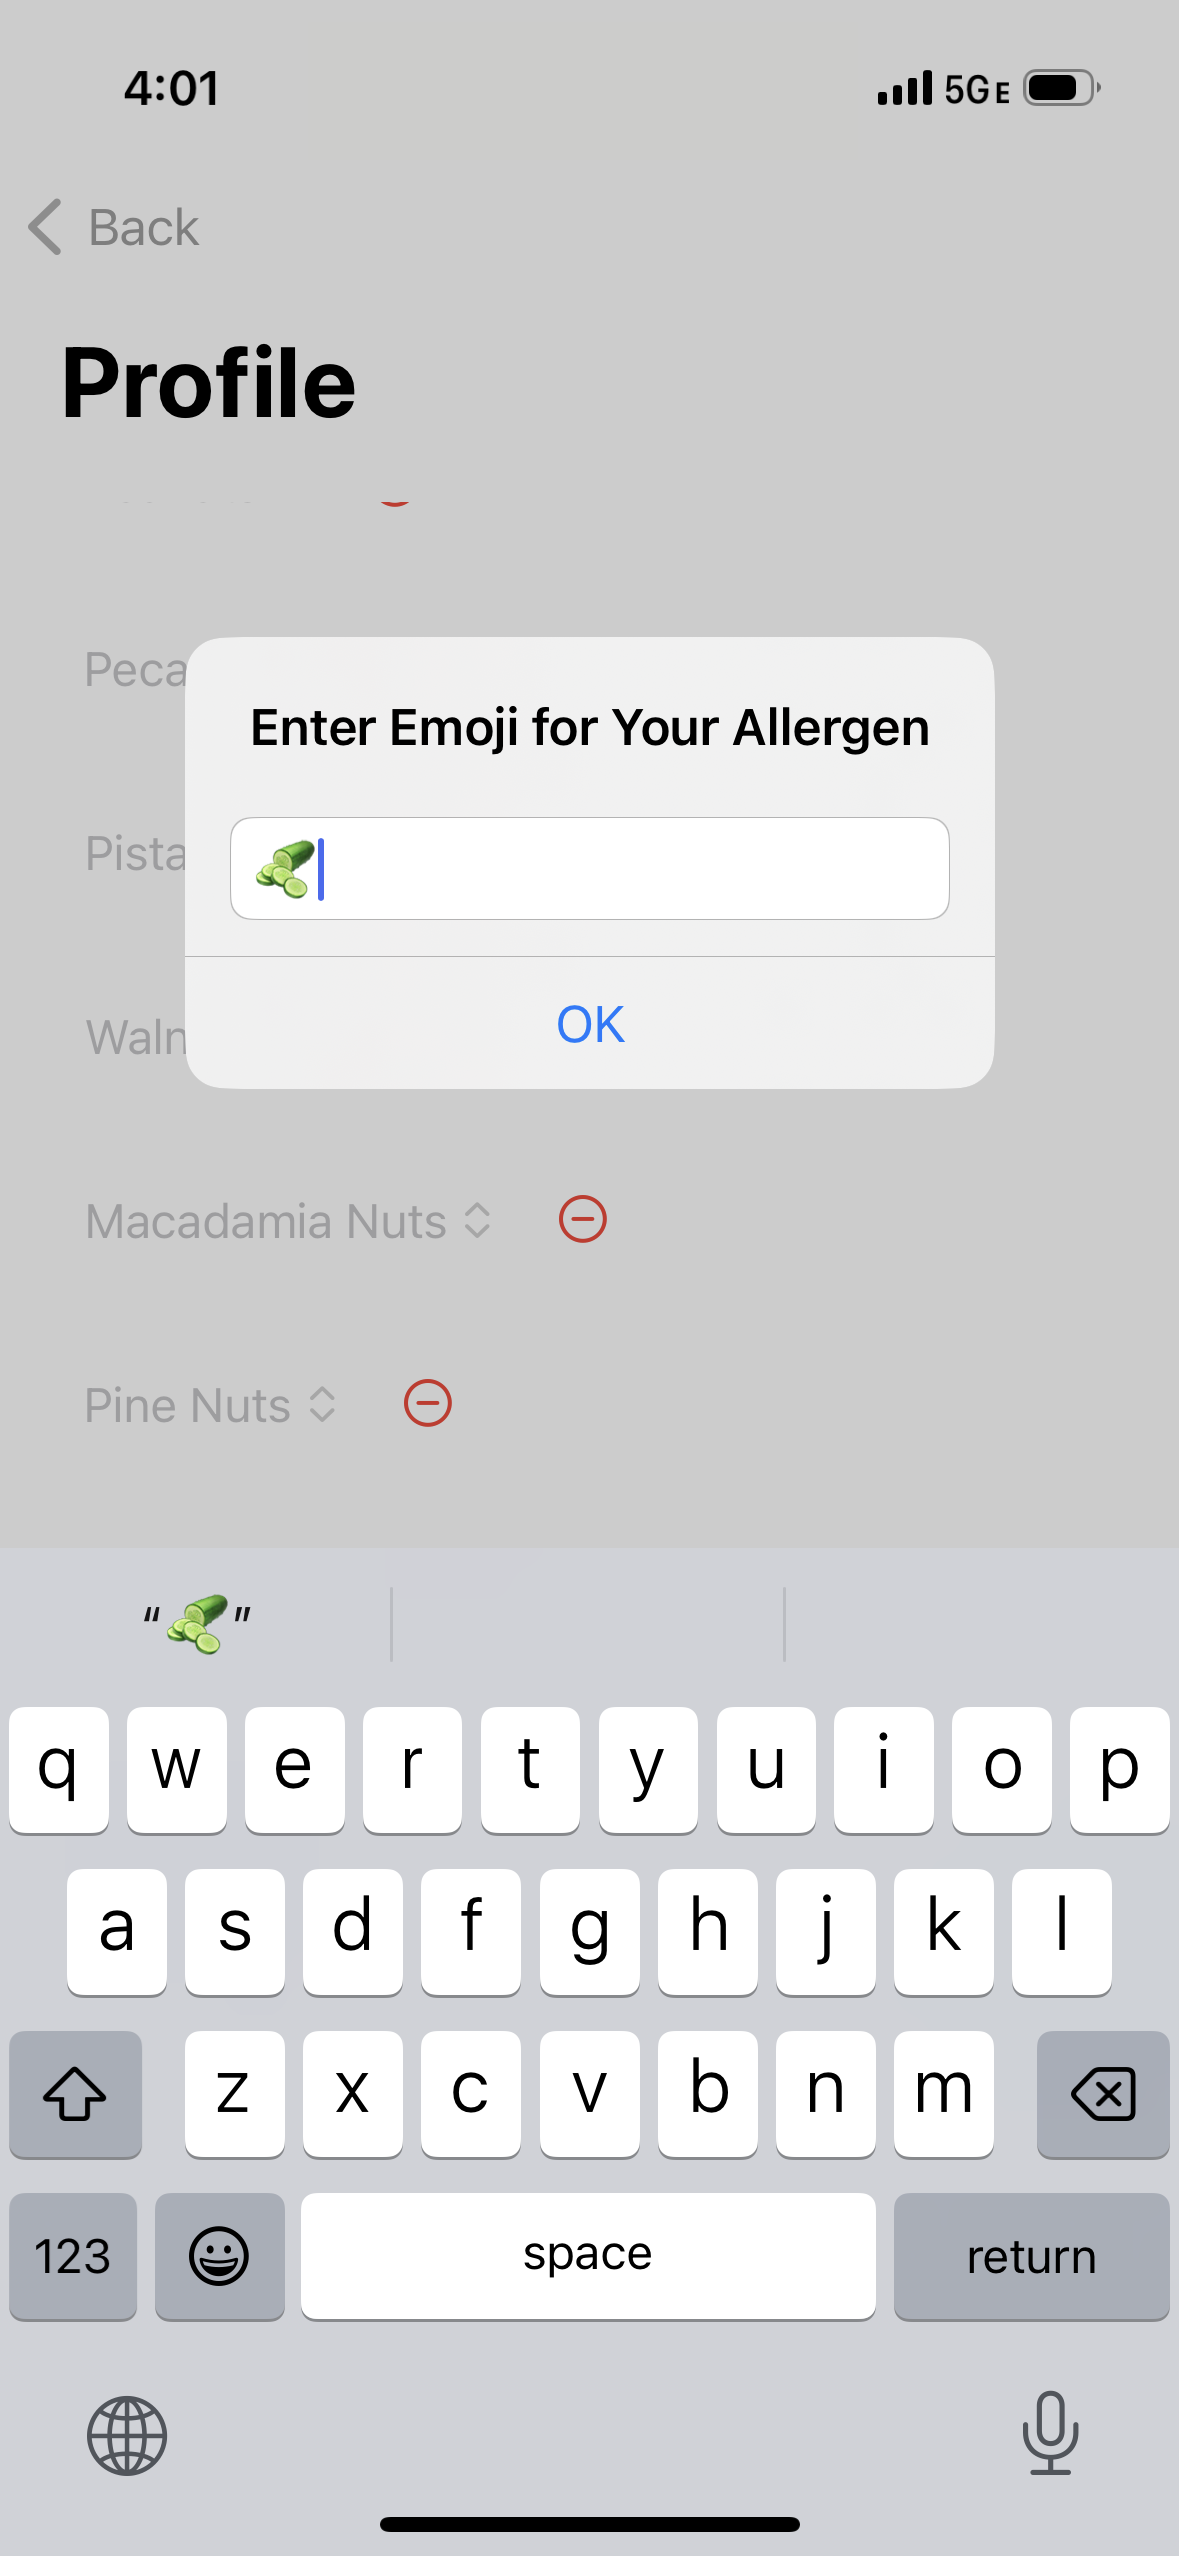
\includegraphics[width=0.25\linewidth]{thesis//chapters//images/otherAllergen4.PNG}
    \caption{User Adding Other Allergen Emoji}
    \label{fig:enter-label}
\end{figure}

Finally, my initial prototype had a "Protect data with FaceID" button, however not every iOS device has FaceID enabled. So, I changed the toggle to say "Protect data with Passcode, TouchID, or FaceID" to account for different iPhone models and security setups. And, depending on the setup, the screen to authenticate will ask for the user's passcode, TouchID, or FaceID.

\begin{figure} [H]
    \centering
    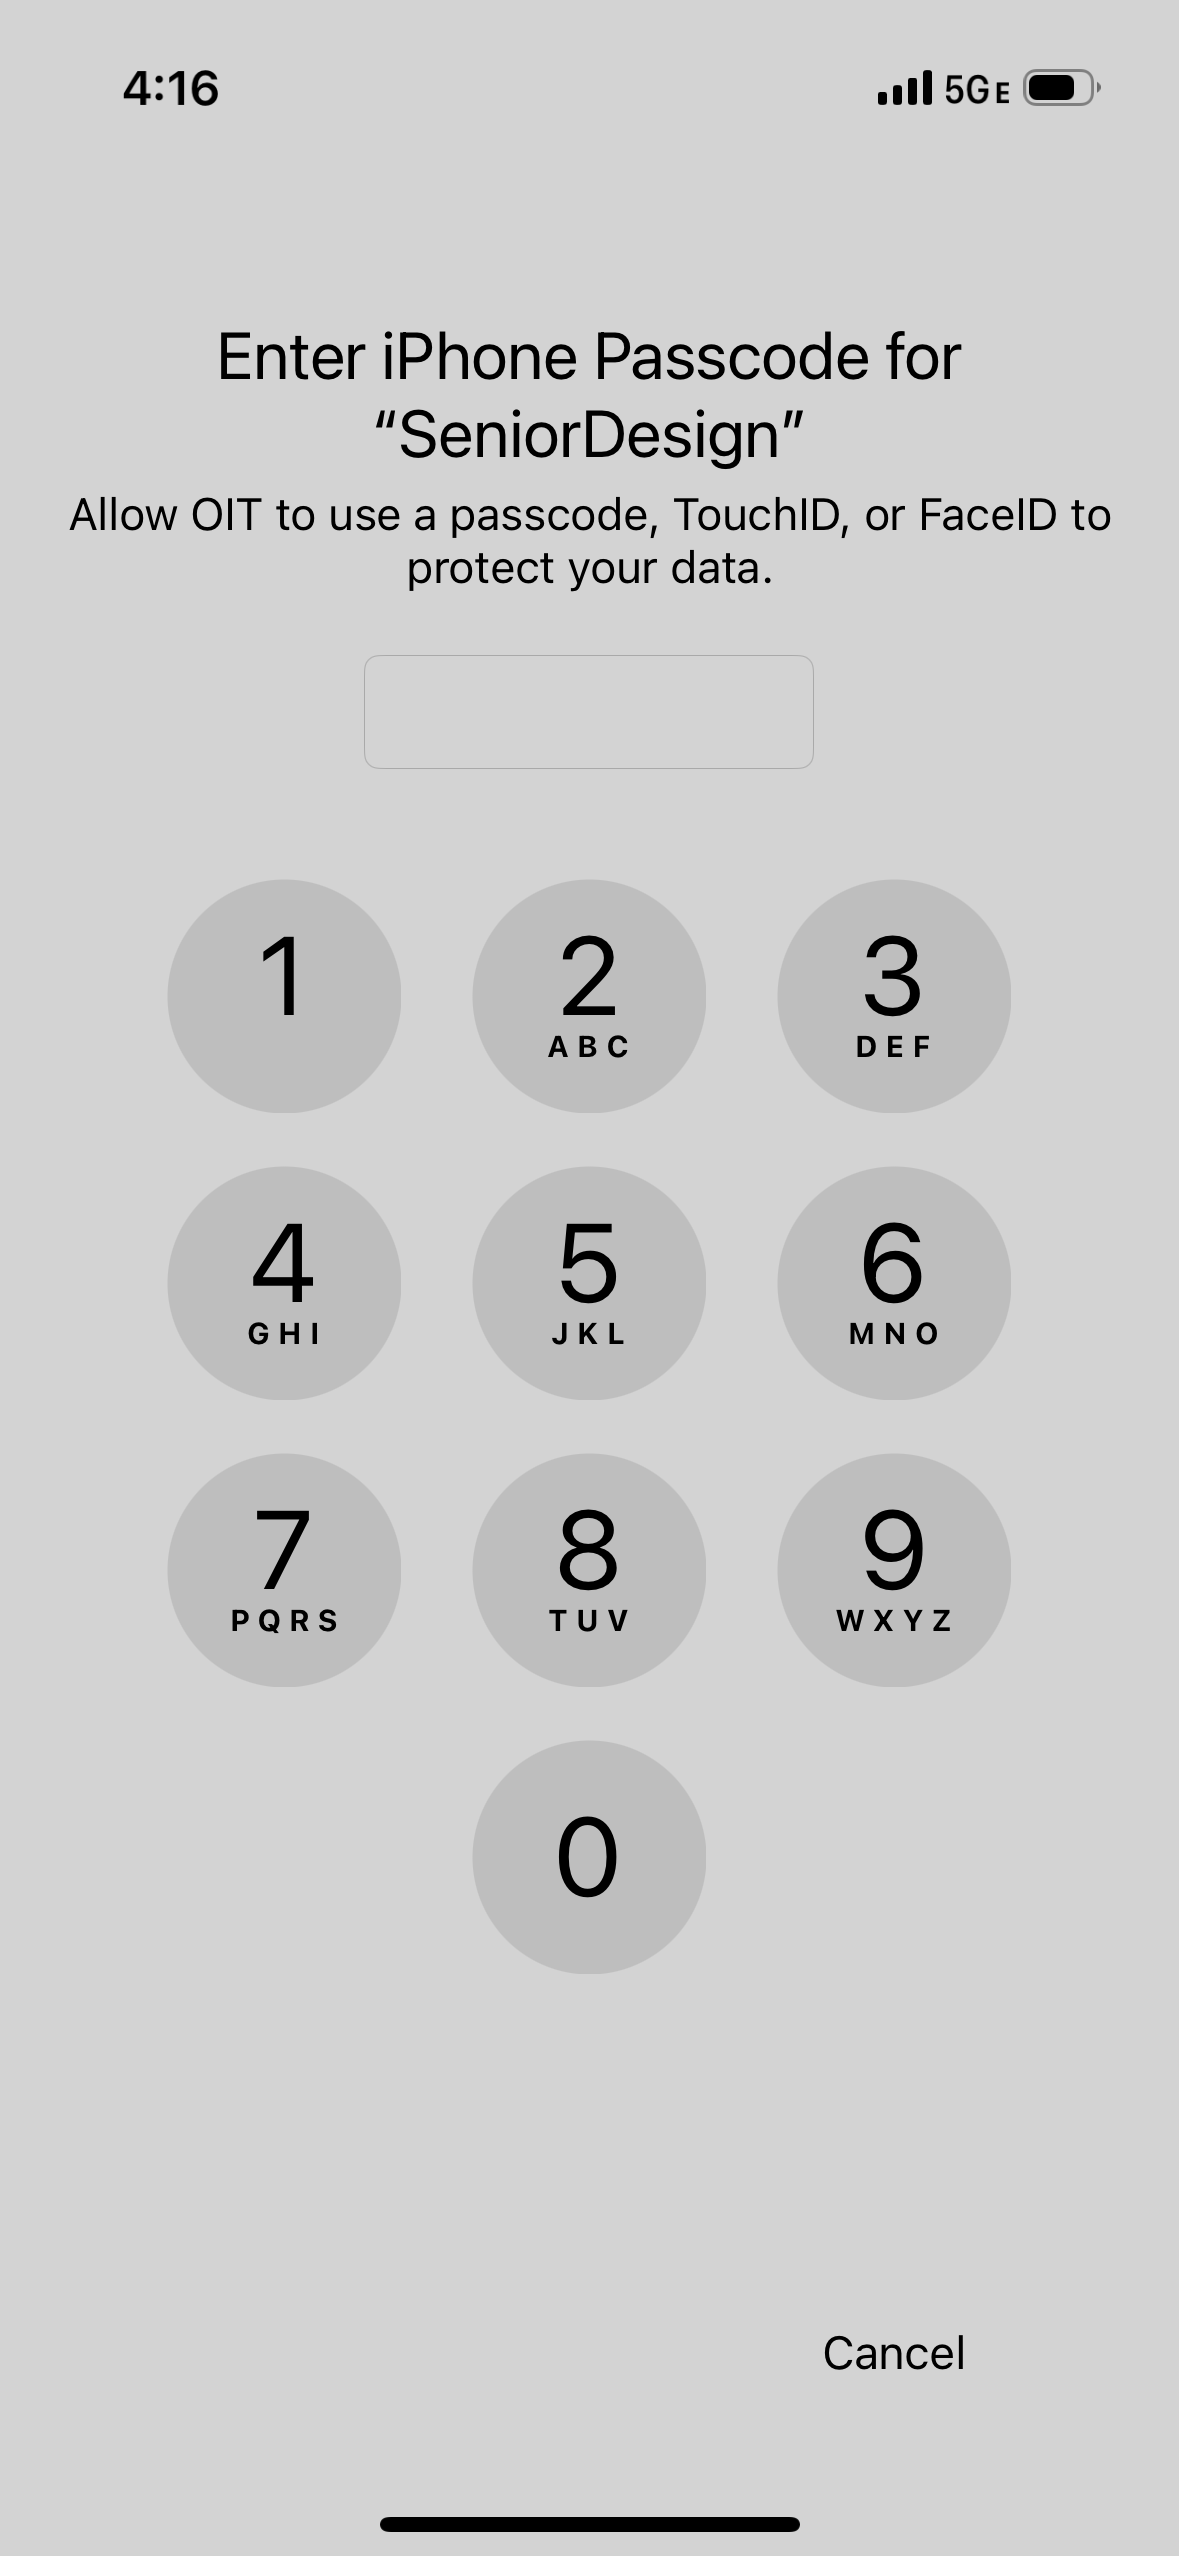
\includegraphics[width=0.25\linewidth]{thesis//chapters//images/passcode.PNG}
    \caption{Screen to Enter Passcode}
    \label{fig:enter-label}
\end{figure}

\subsection{Dosing Tab Changes}

The Dosing tab of the app went through several iterations after the prototypes were made. Instead of having a large list of all the allergens and doses, I separated the sections and made them collapsable, allowing the user to more easily navigate through the doses.

\begin{figure} [H]
    \centering
    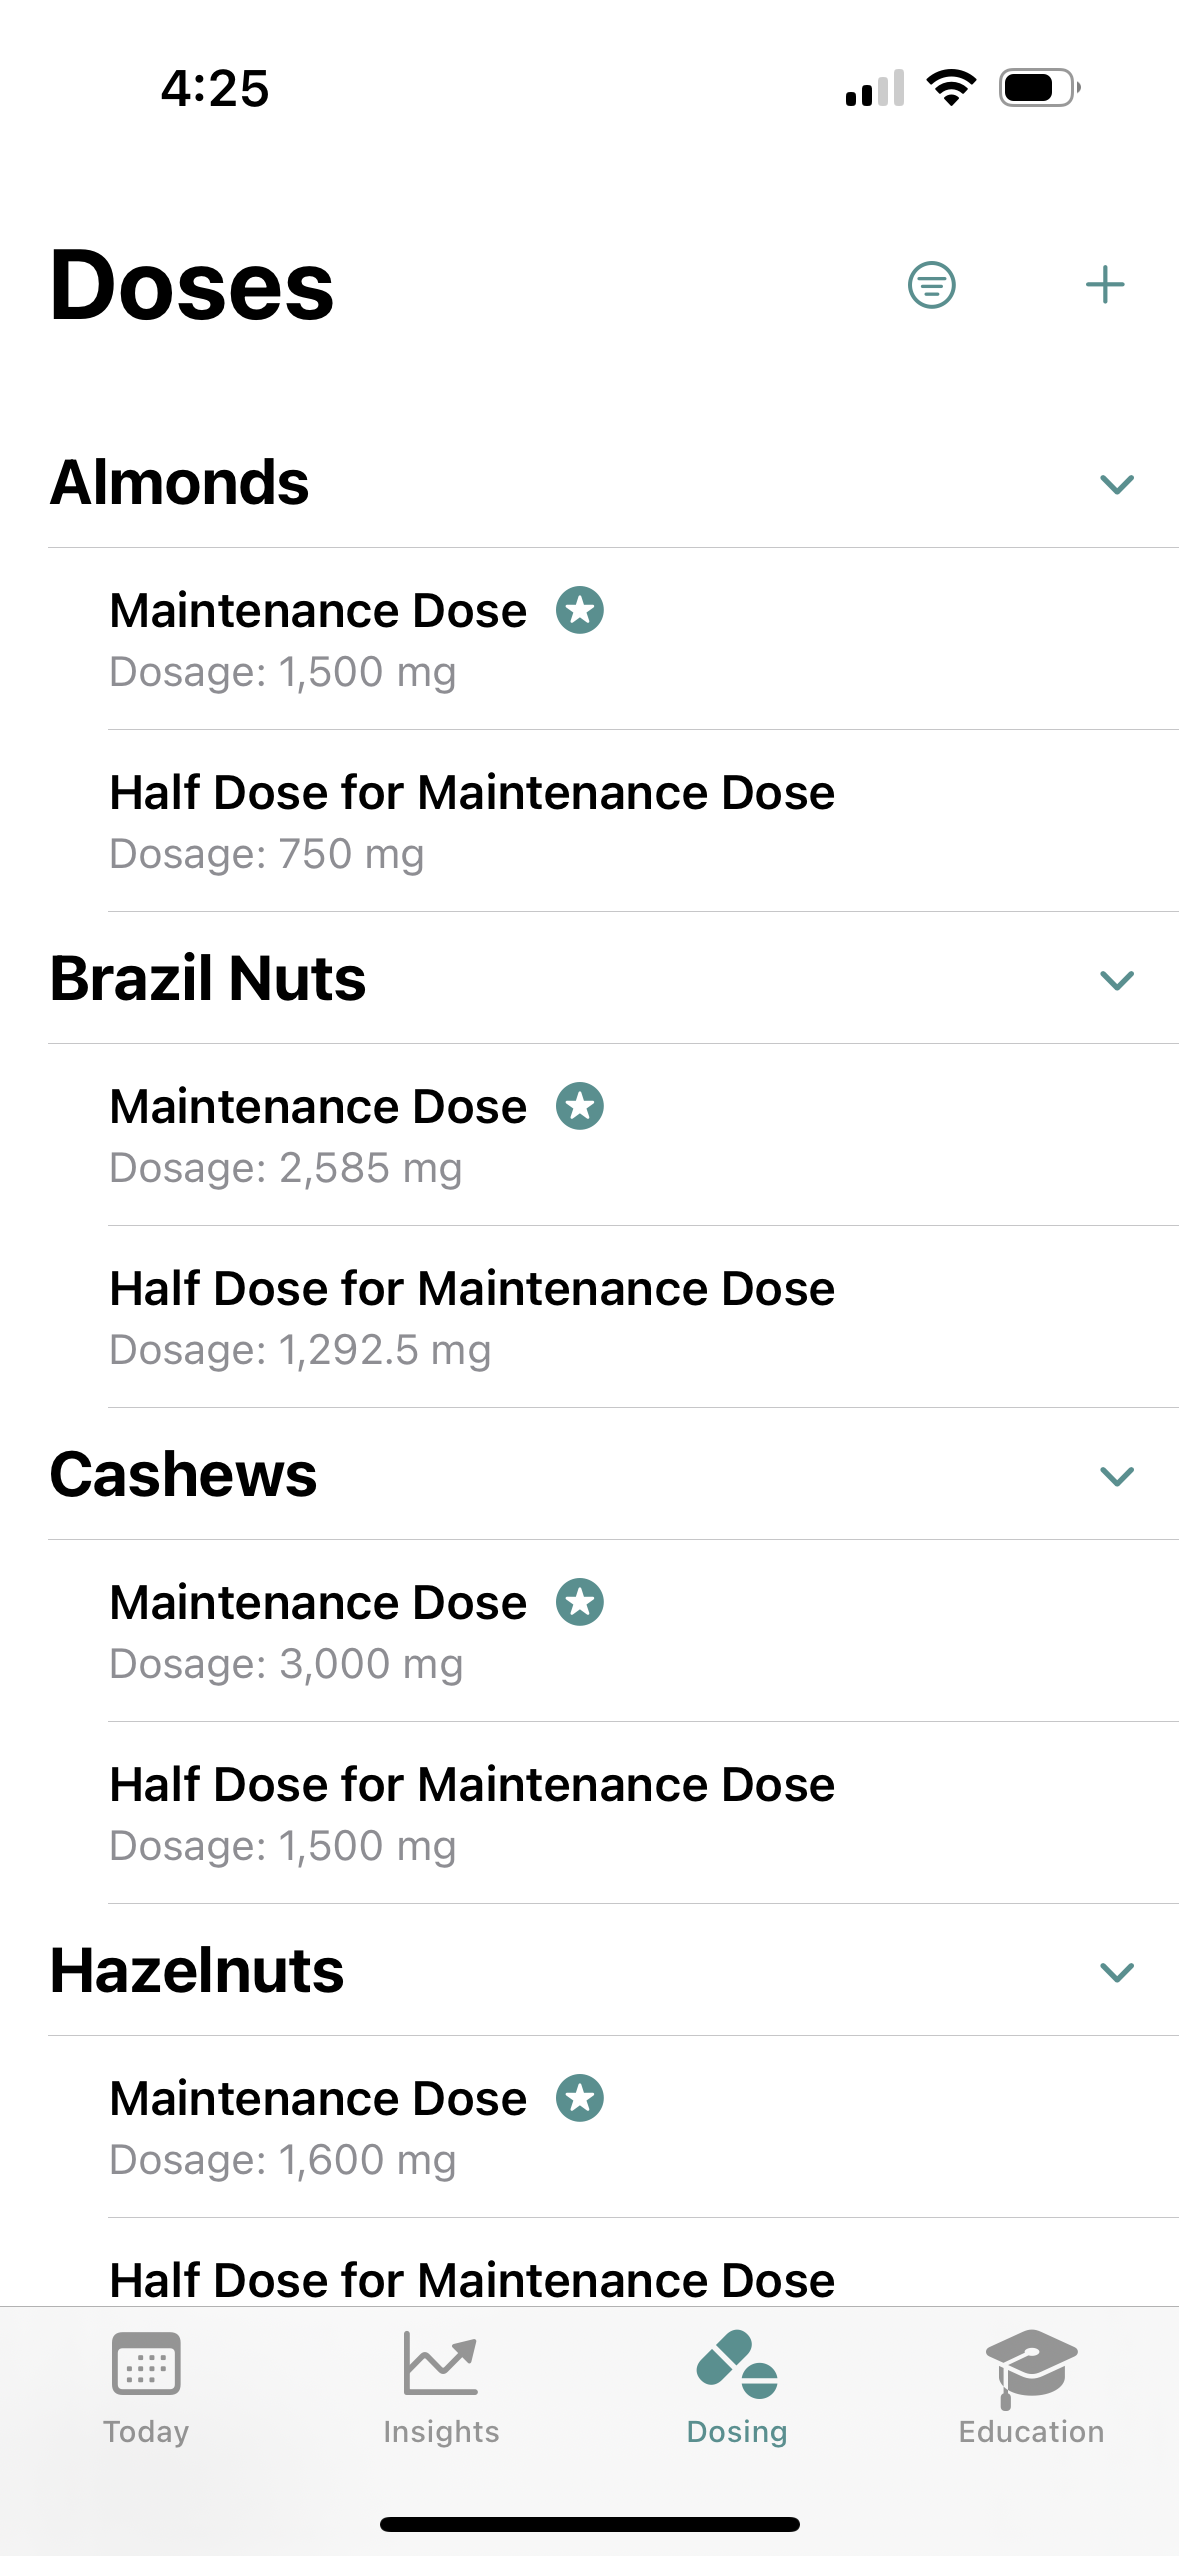
\includegraphics[width=0.25\linewidth]{thesis//chapters//images/dosingTabUnfiltered.PNG}
    \caption{Uncollapsed Sections of Dosing Tab}
    \label{fig:enter-label}
\end{figure}

\begin{figure} [H]
    \centering
    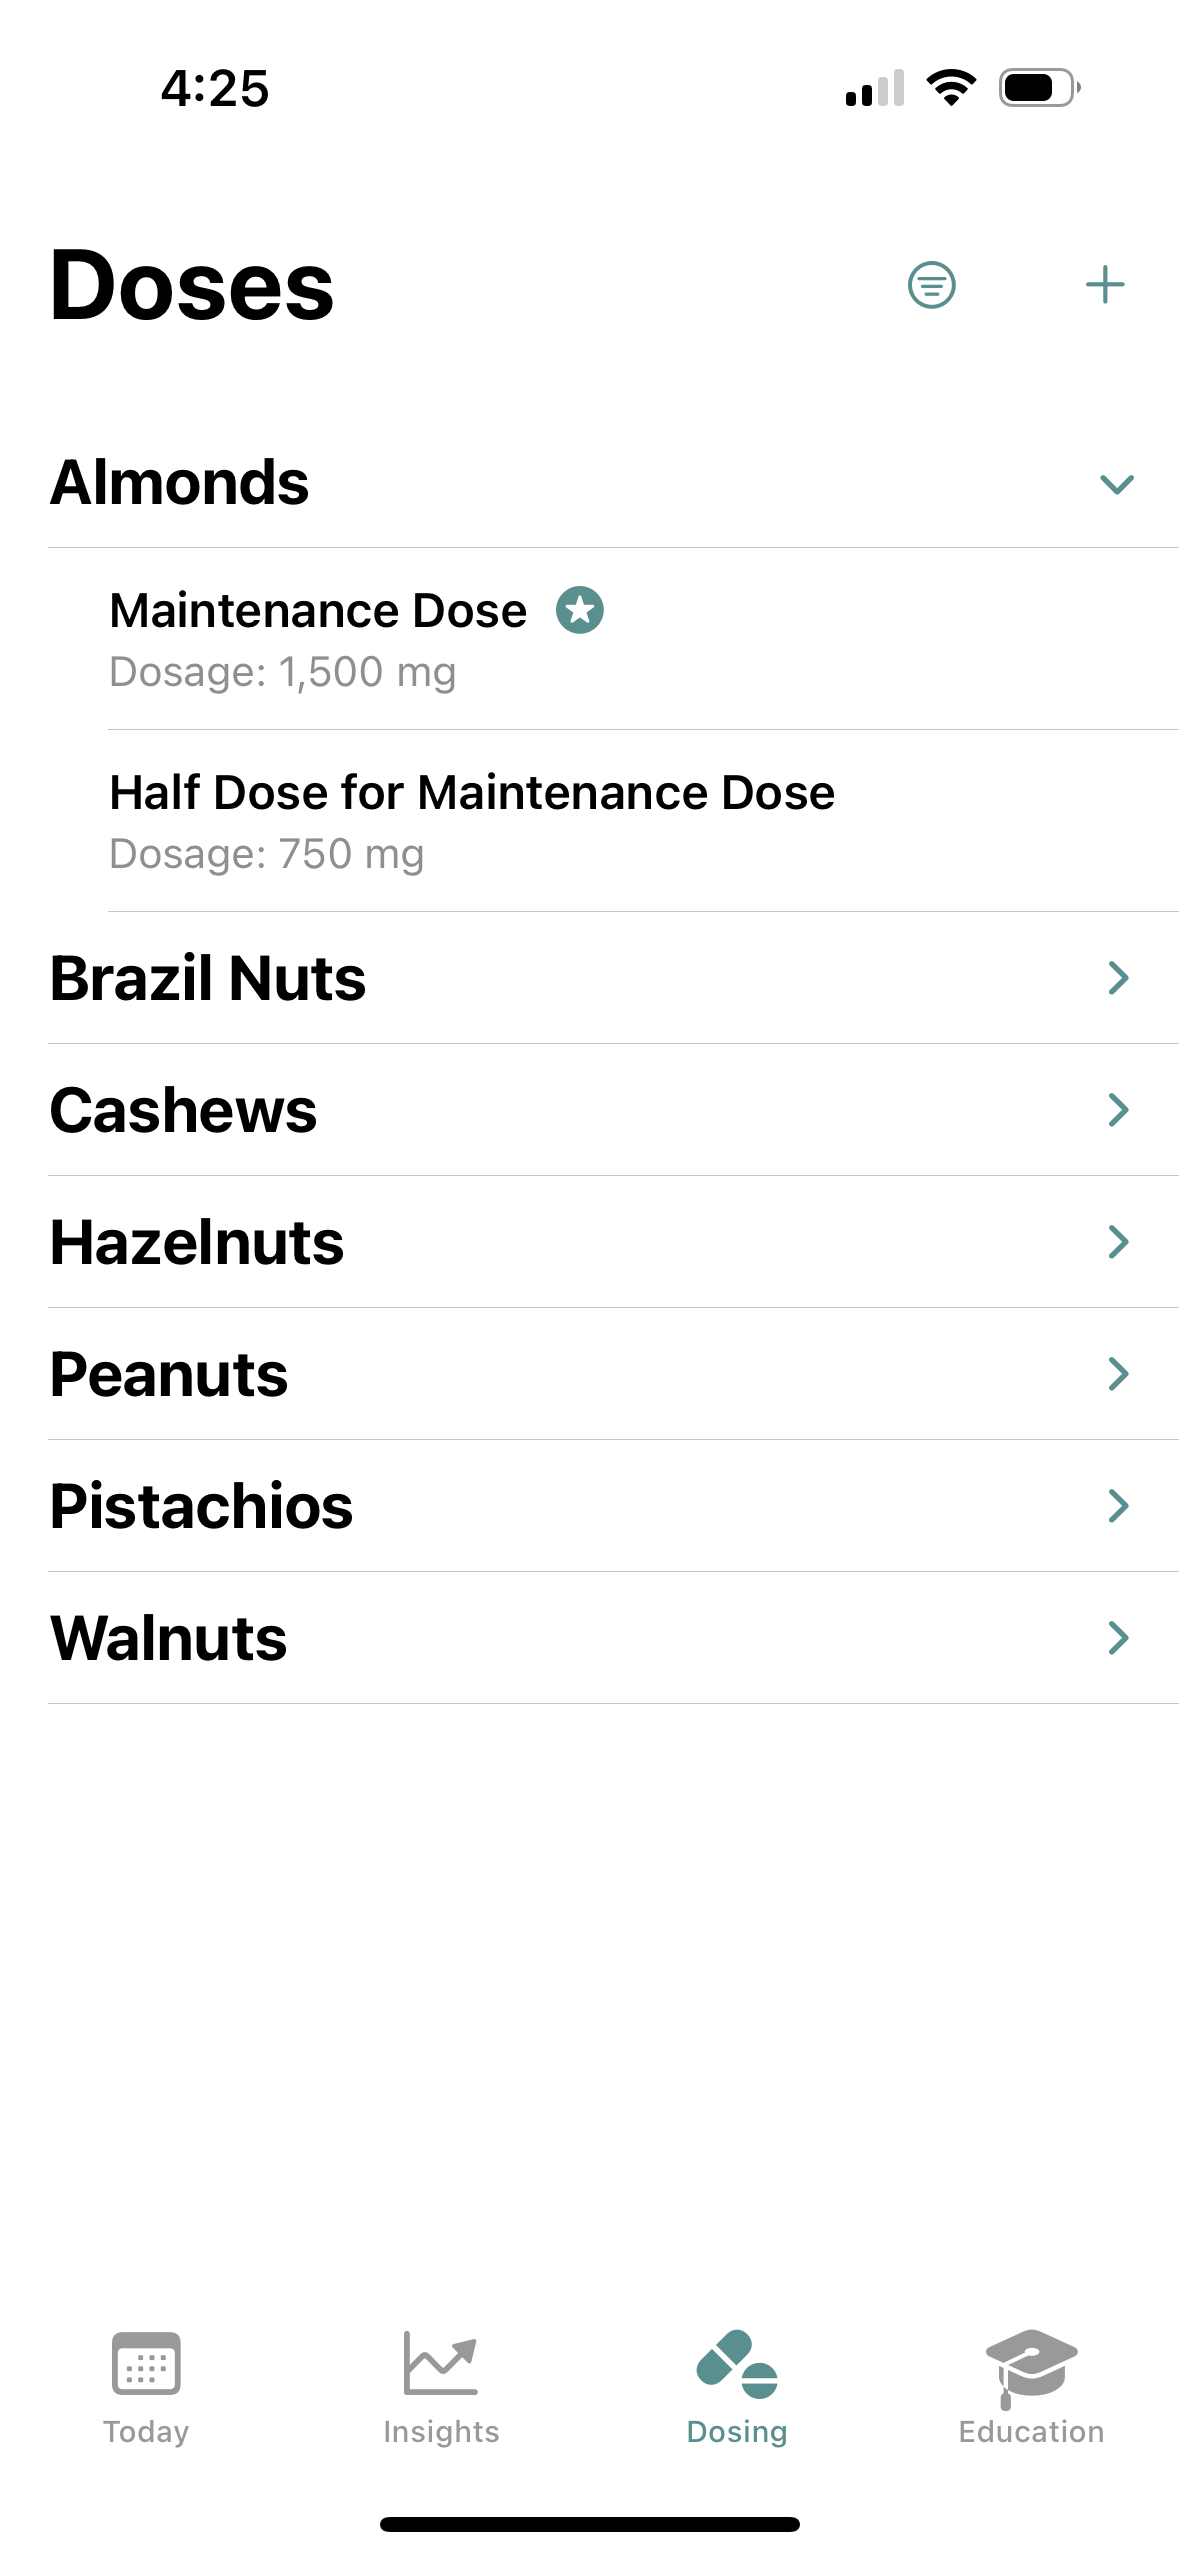
\includegraphics[width=0.25\linewidth]{thesis//chapters//images/dosingTabCollapsed2.PNG}
    \caption{Collapsed Sections of Dosing Tab}
    \label{fig:enter-label}
\end{figure}

Additionally, I added the ability to mark which dose is your current dose, filter the tab only to show current doses, and edit or delete doses.

\begin{figure} [H]
    \centering
    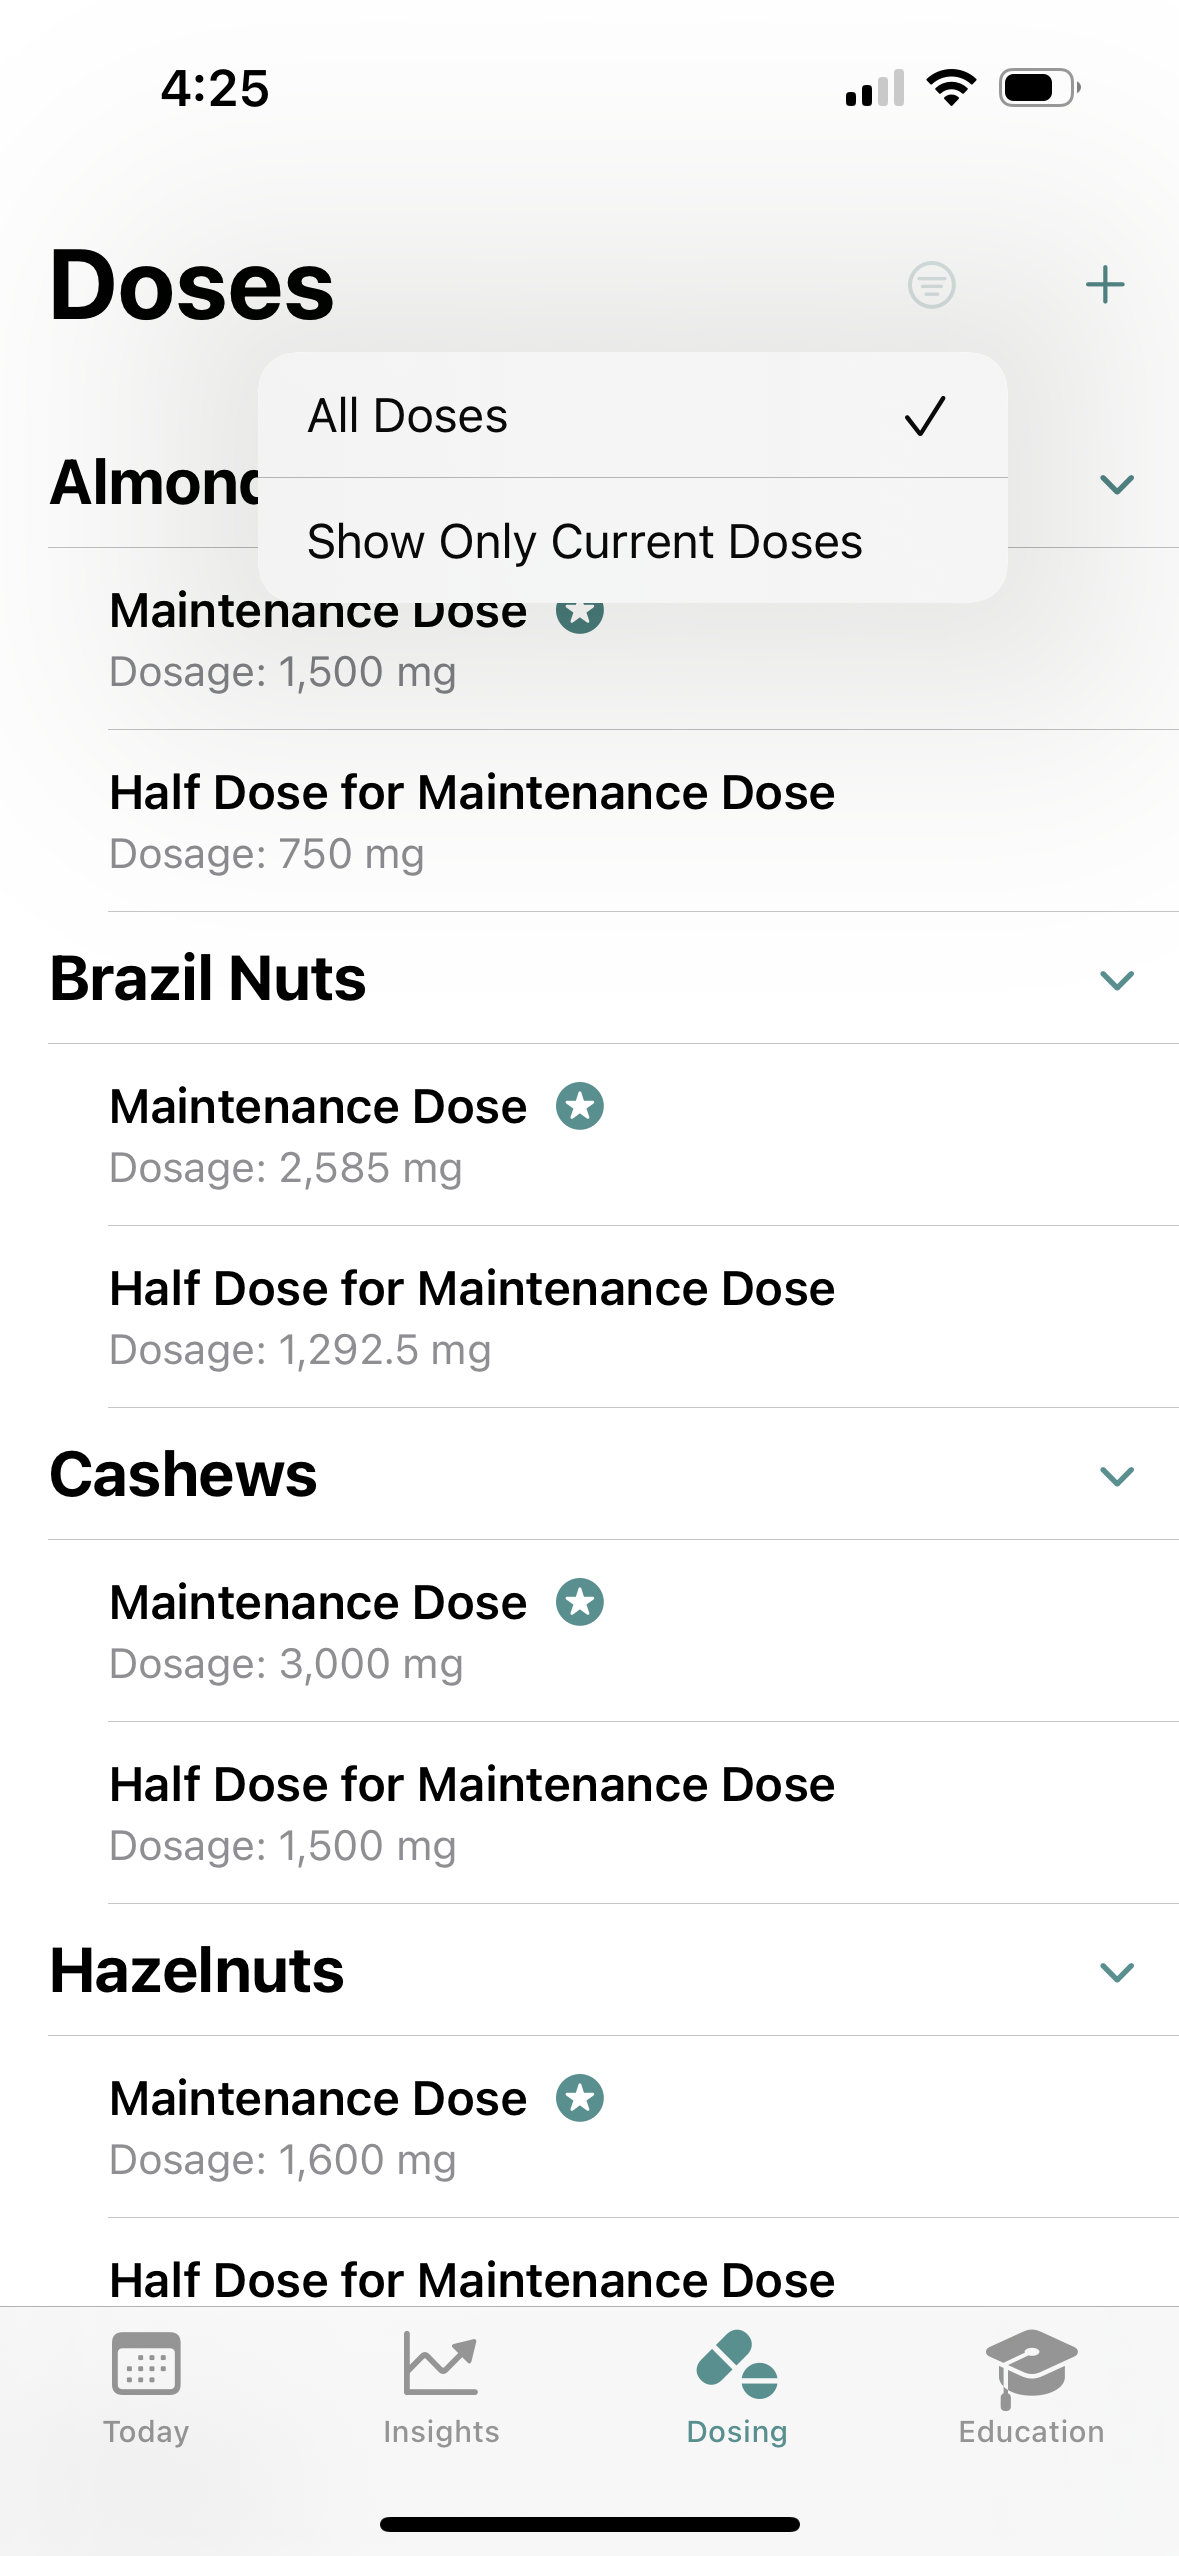
\includegraphics[width=0.25\linewidth]{thesis//chapters//images/dosingTabFilters.PNG}
    \caption{Dosing Tab Filters}
    \label{fig:enter-label}
\end{figure}

\begin{figure} [H]
    \centering
    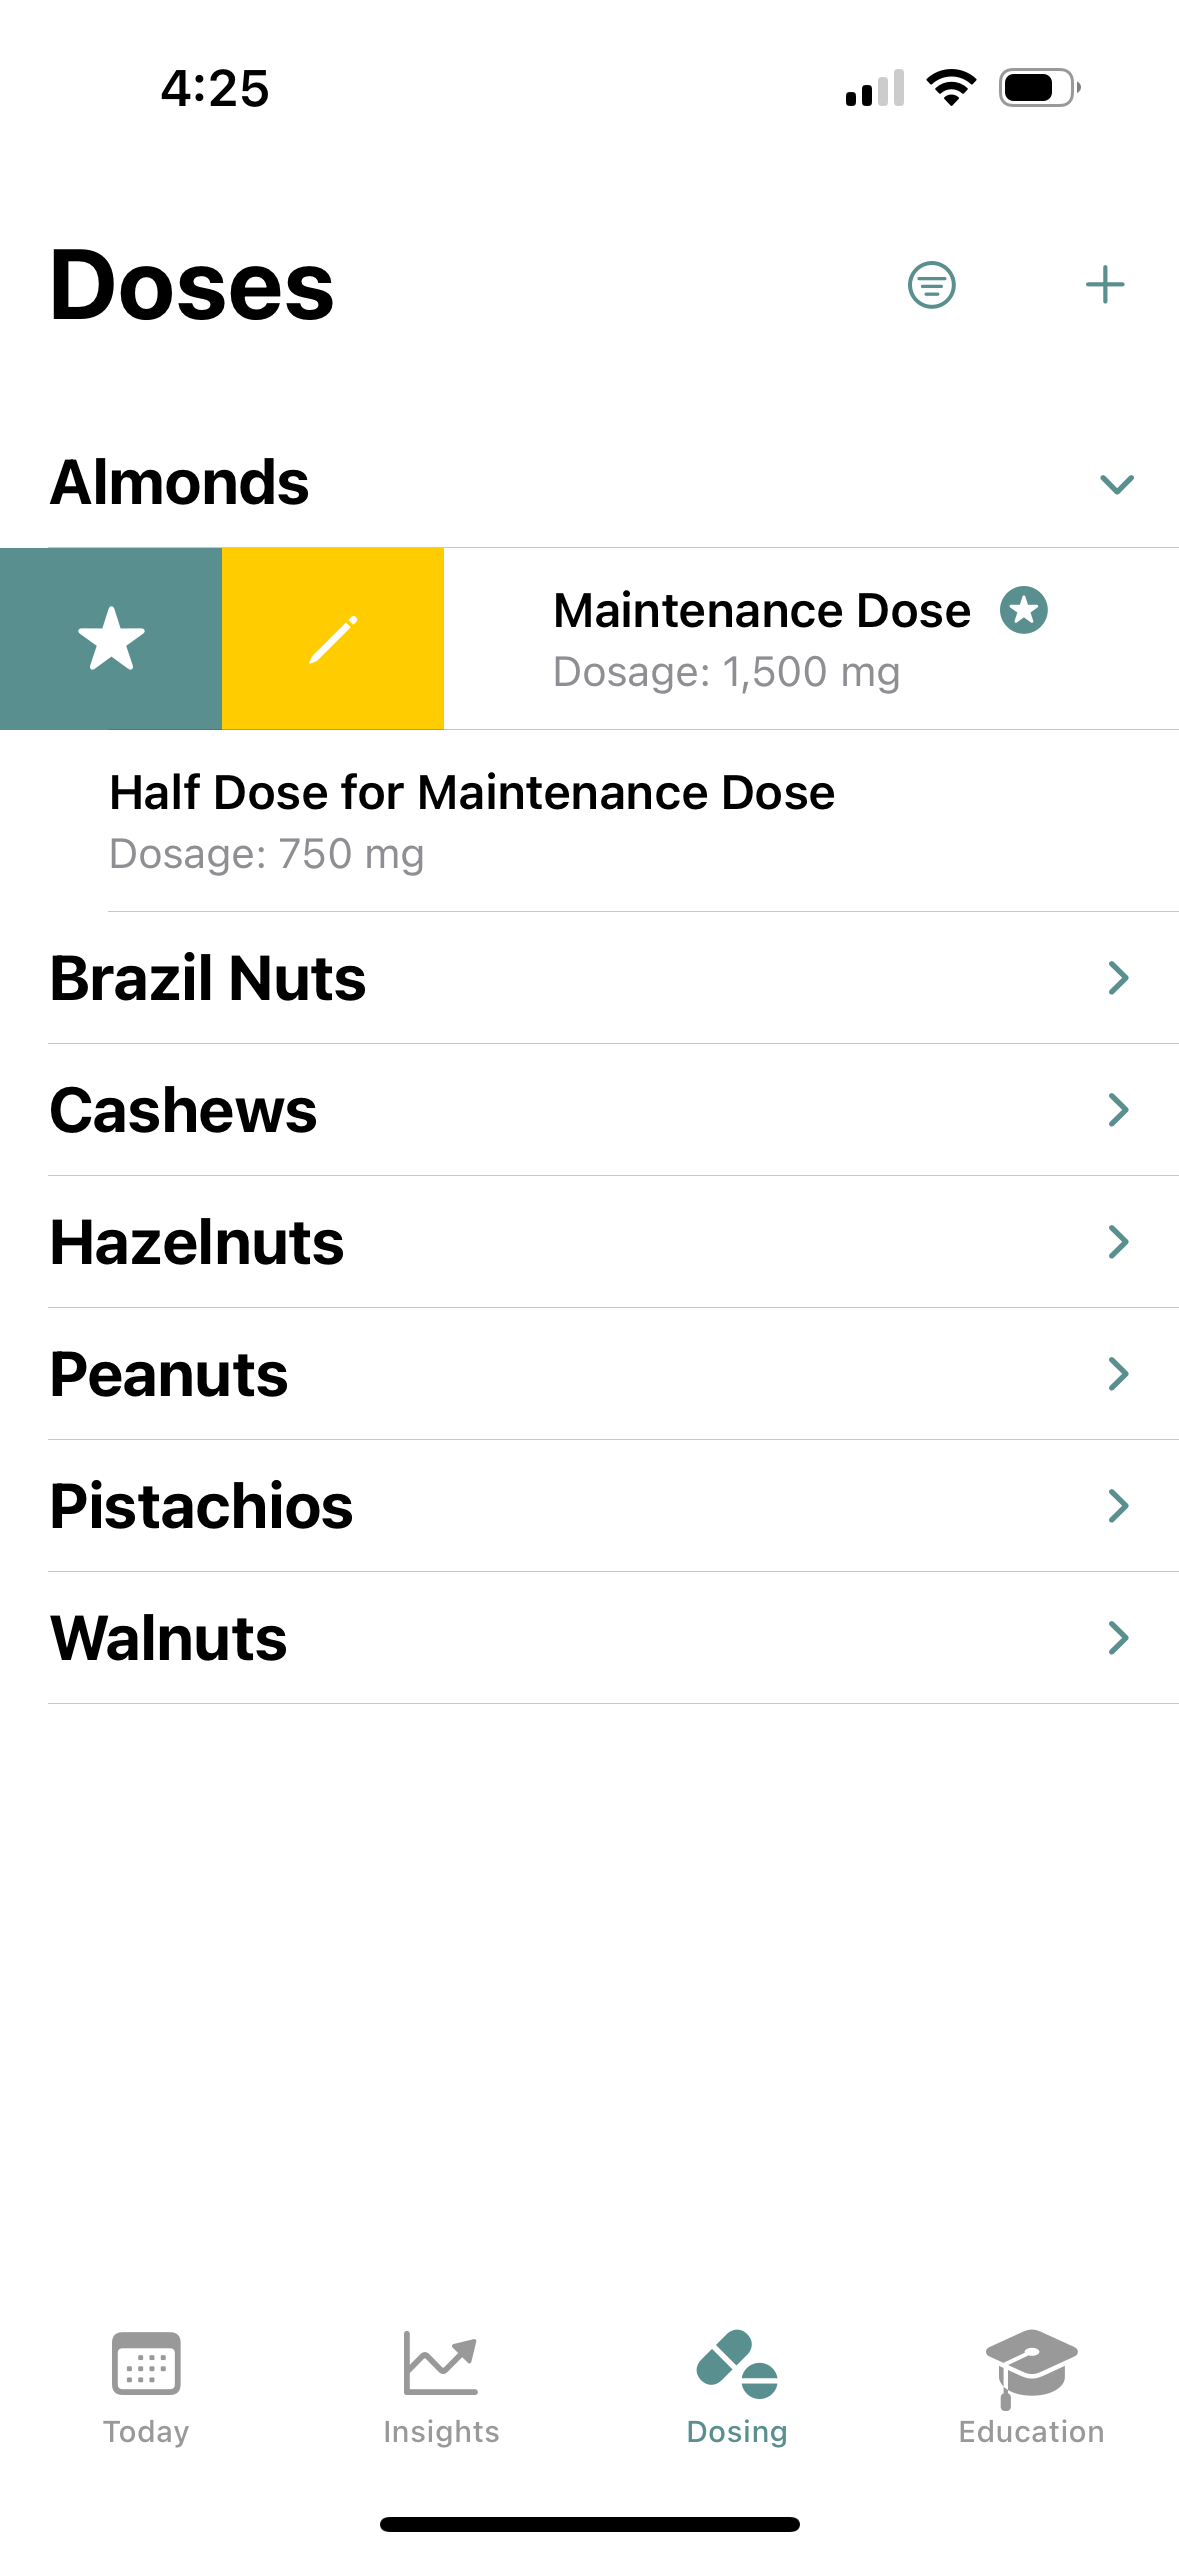
\includegraphics[width=0.25\linewidth]{thesis//chapters//images/dosingTabEditActions.PNG}
    \caption{Dose Edit Actions}
    \label{fig:enter-label}
\end{figure}

\begin{figure} [H]
    \centering
    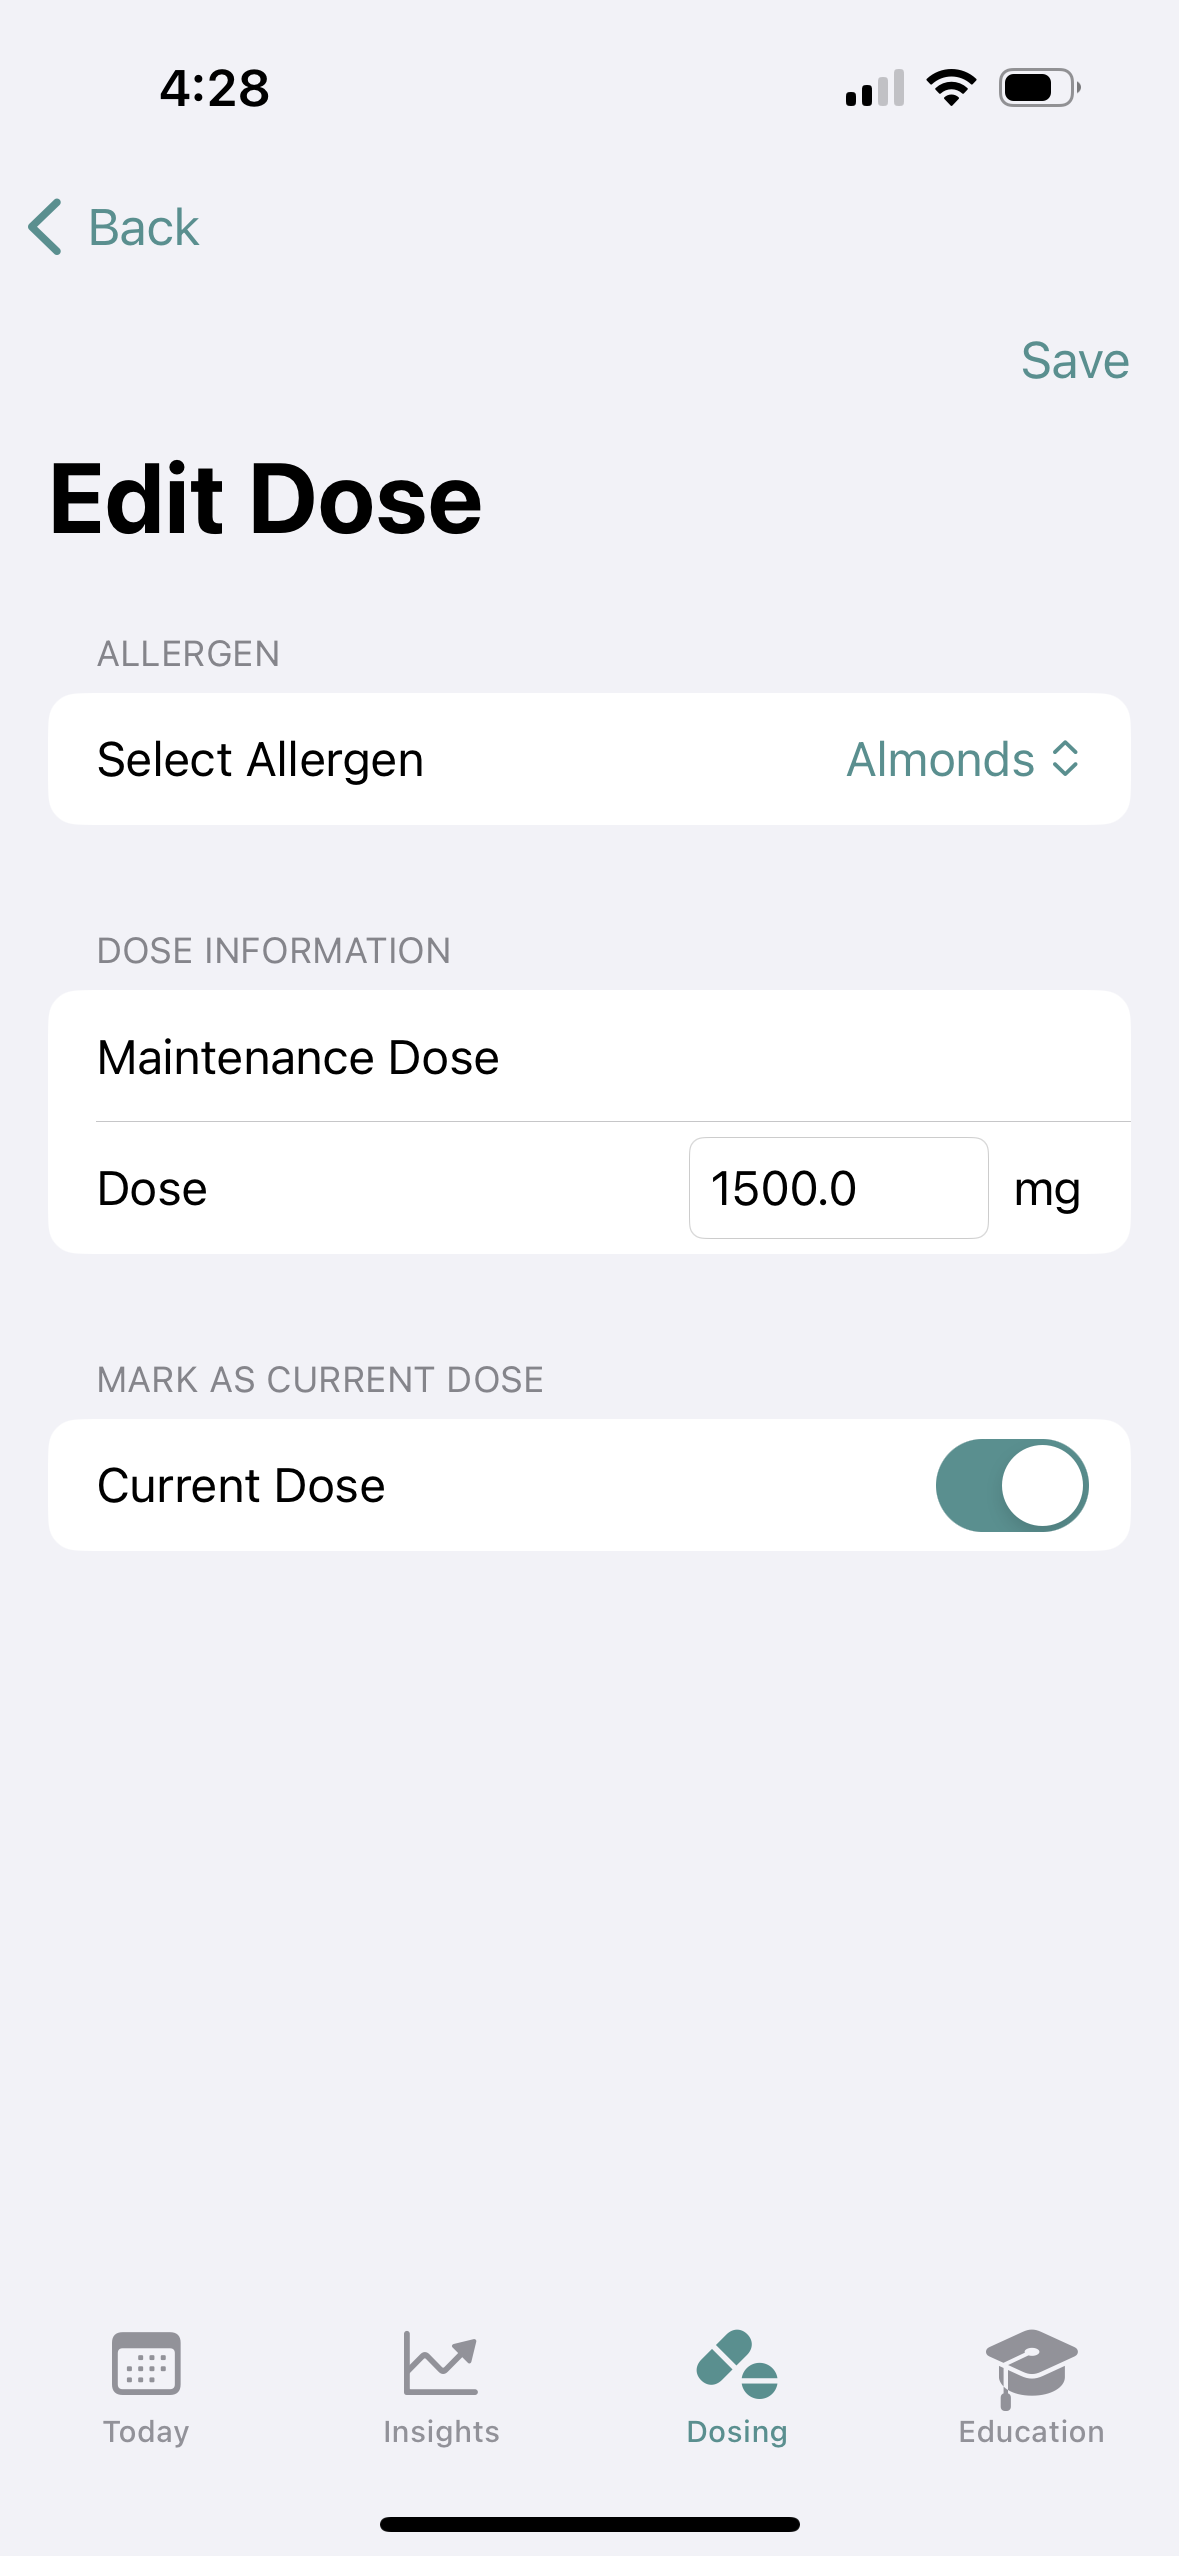
\includegraphics[width=0.25\linewidth]{thesis//chapters//images/dosingTabEditScreen.PNG}
    \caption{Dose Edit Screen}
    \label{fig:enter-label}
\end{figure}

\begin{figure} [H]
    \centering
    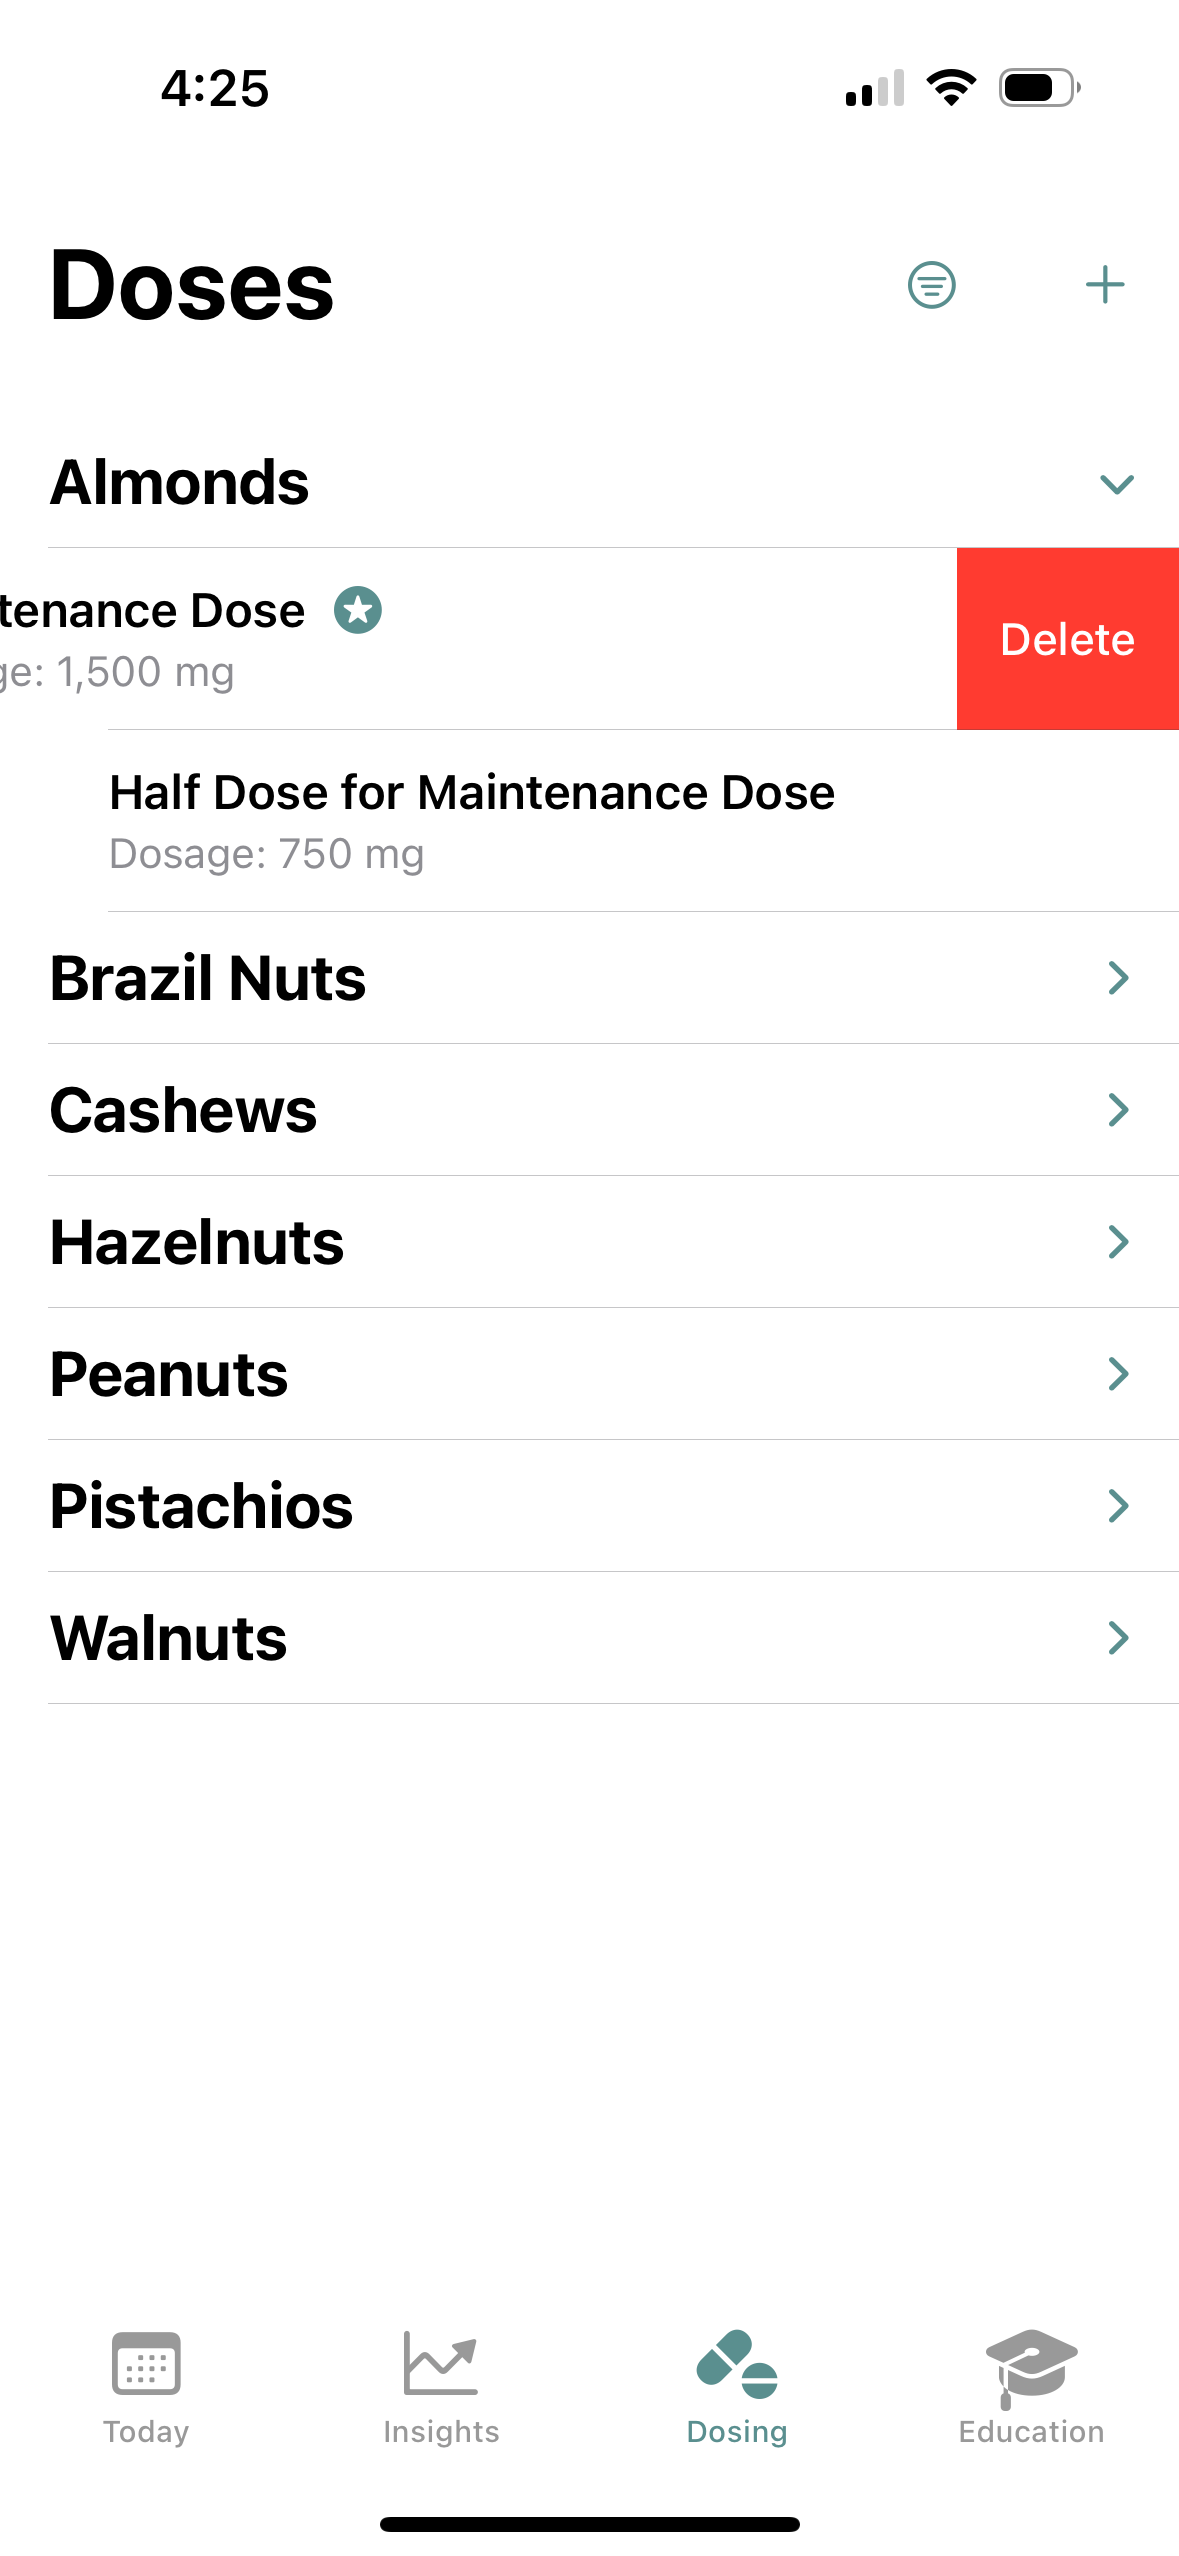
\includegraphics[width=0.25\linewidth]{thesis//chapters//images/dosingTabDelete.PNG}
    \caption{Dose Delete Action}
    \label{fig:enter-label}
\end{figure}

\section{User Guide}

After finishing developing my application, I created a comprehensive user guide for it, as you can see below.

\begin{figure} [H]
    \centering
    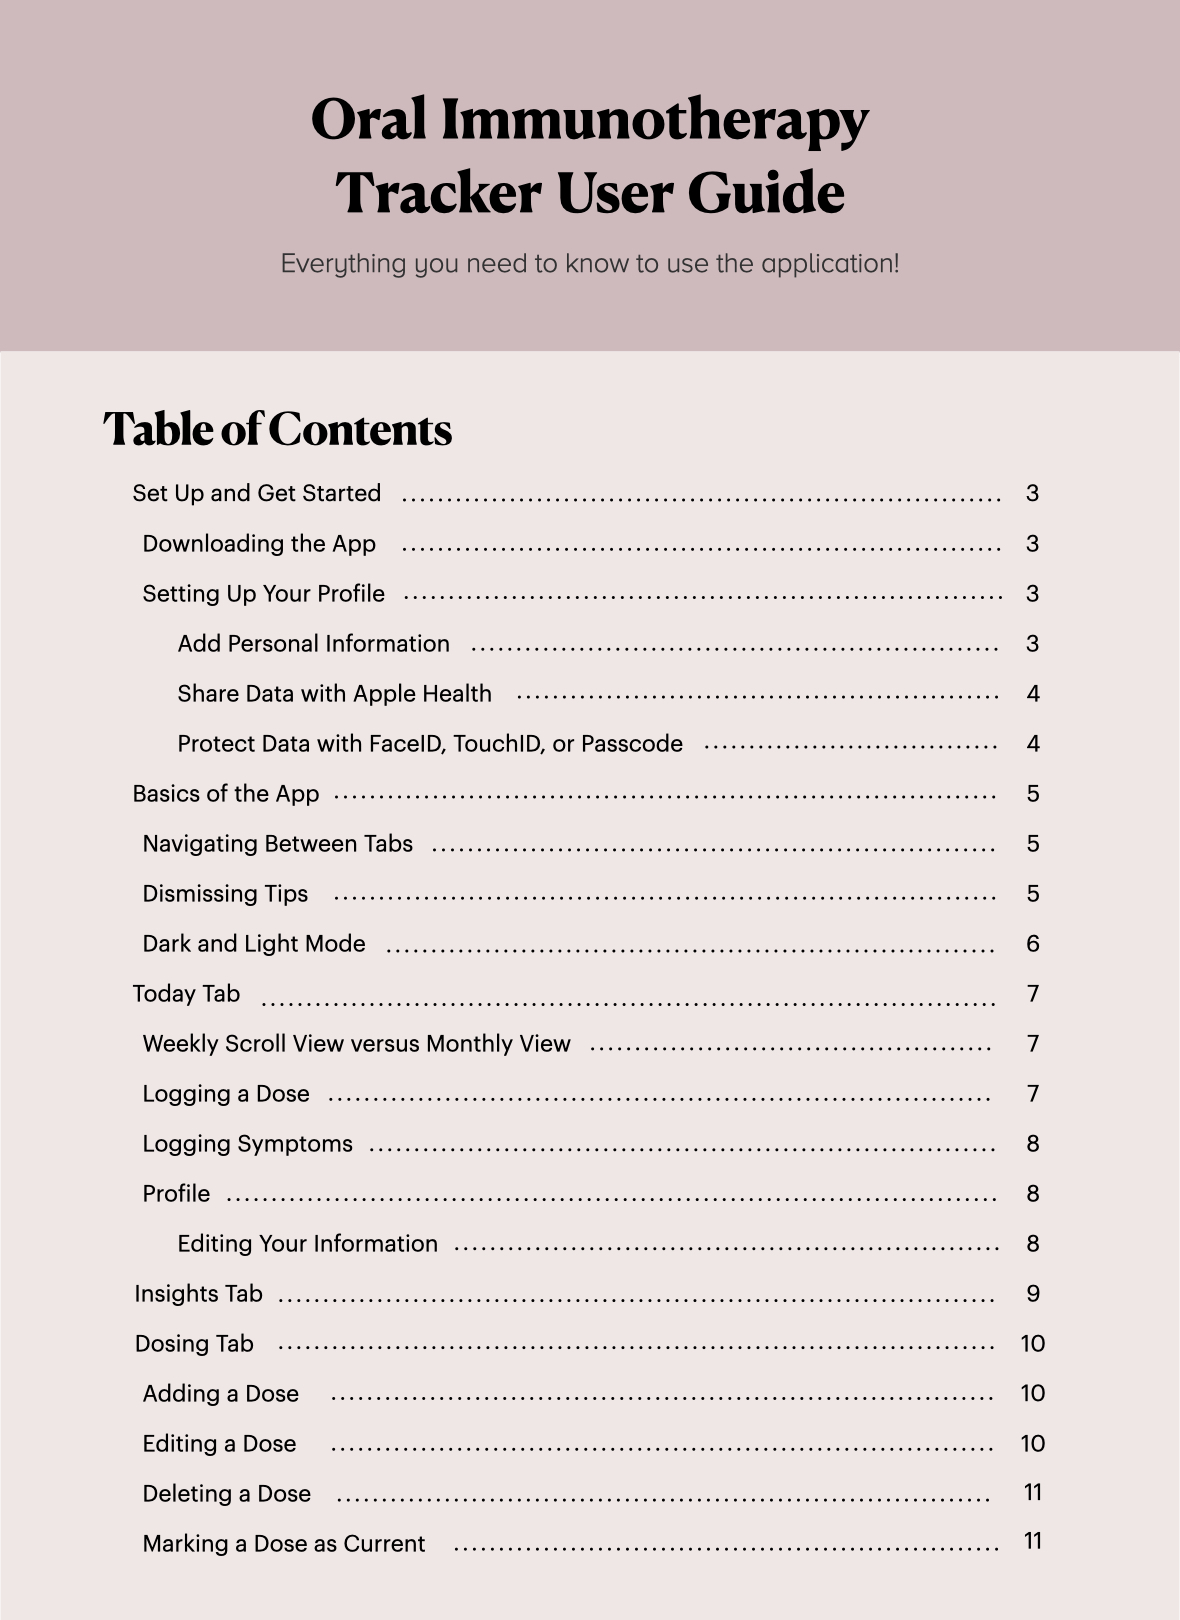
\includegraphics[width=1\linewidth]{thesis//chapters//images/User Guide.001.jpeg}
    \caption{User Guide Page 1}
    \label{fig:enter-label}
\end{figure}

\begin{figure} [H]
    \centering
    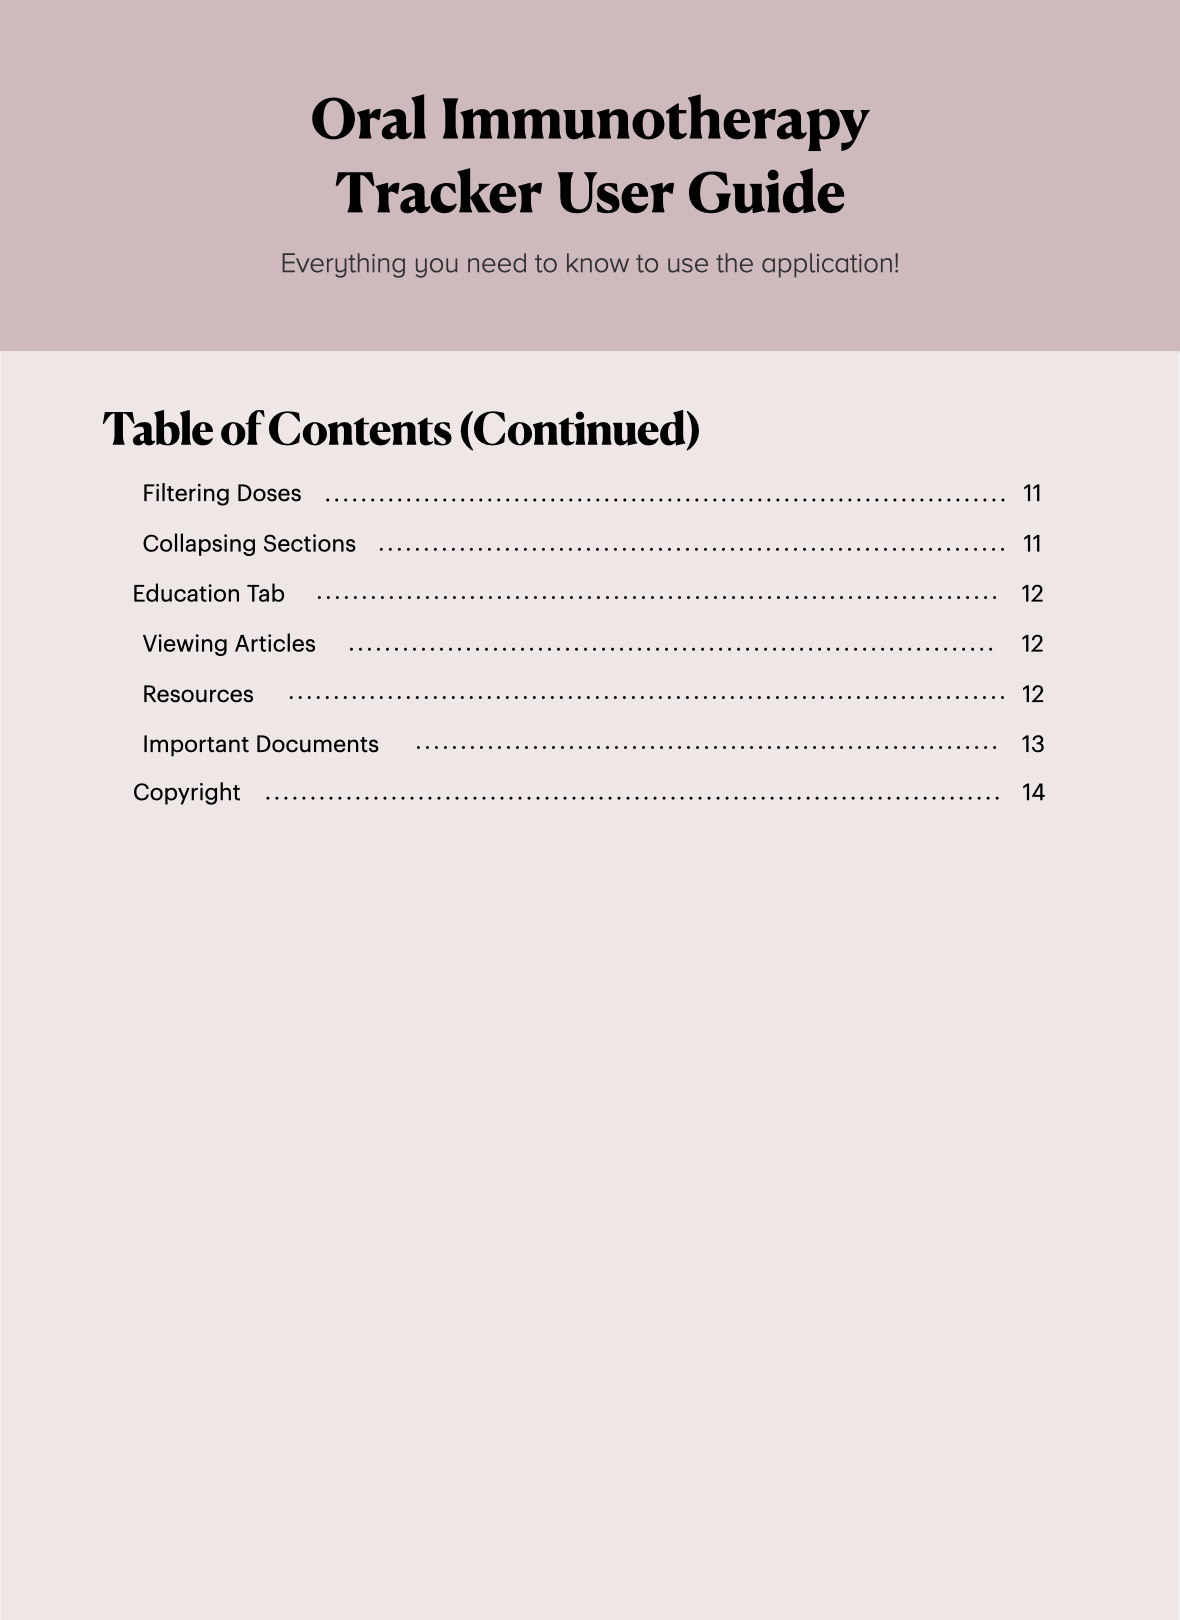
\includegraphics[width=1\linewidth]{thesis//chapters//images/User Guide.002.jpeg}
    \caption{User Guide Page 2}
    \label{fig:enter-label}
\end{figure}

\begin{figure} [H]
    \centering
    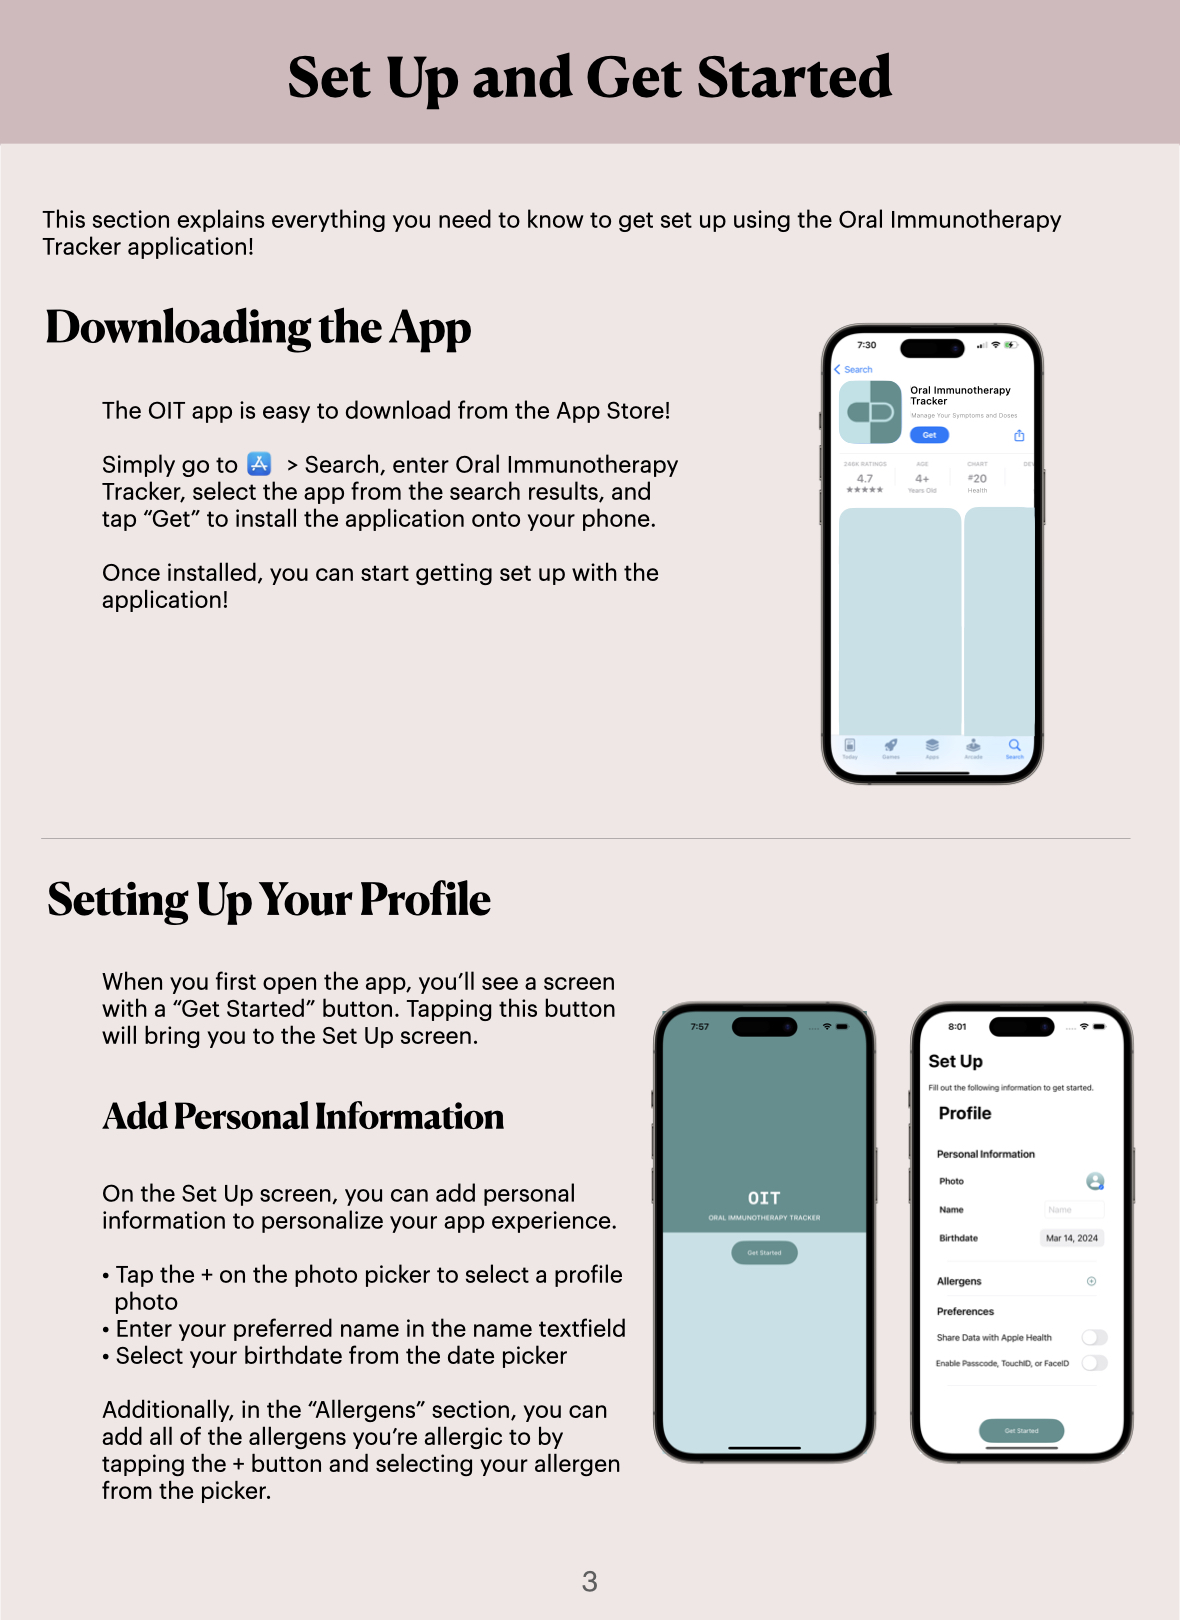
\includegraphics[width=1\linewidth]{thesis//chapters//images/User Guide.003.jpeg}
    \caption{User Guide Page 3}
    \label{fig:enter-label}
\end{figure}

\begin{figure} [H]
    \centering
    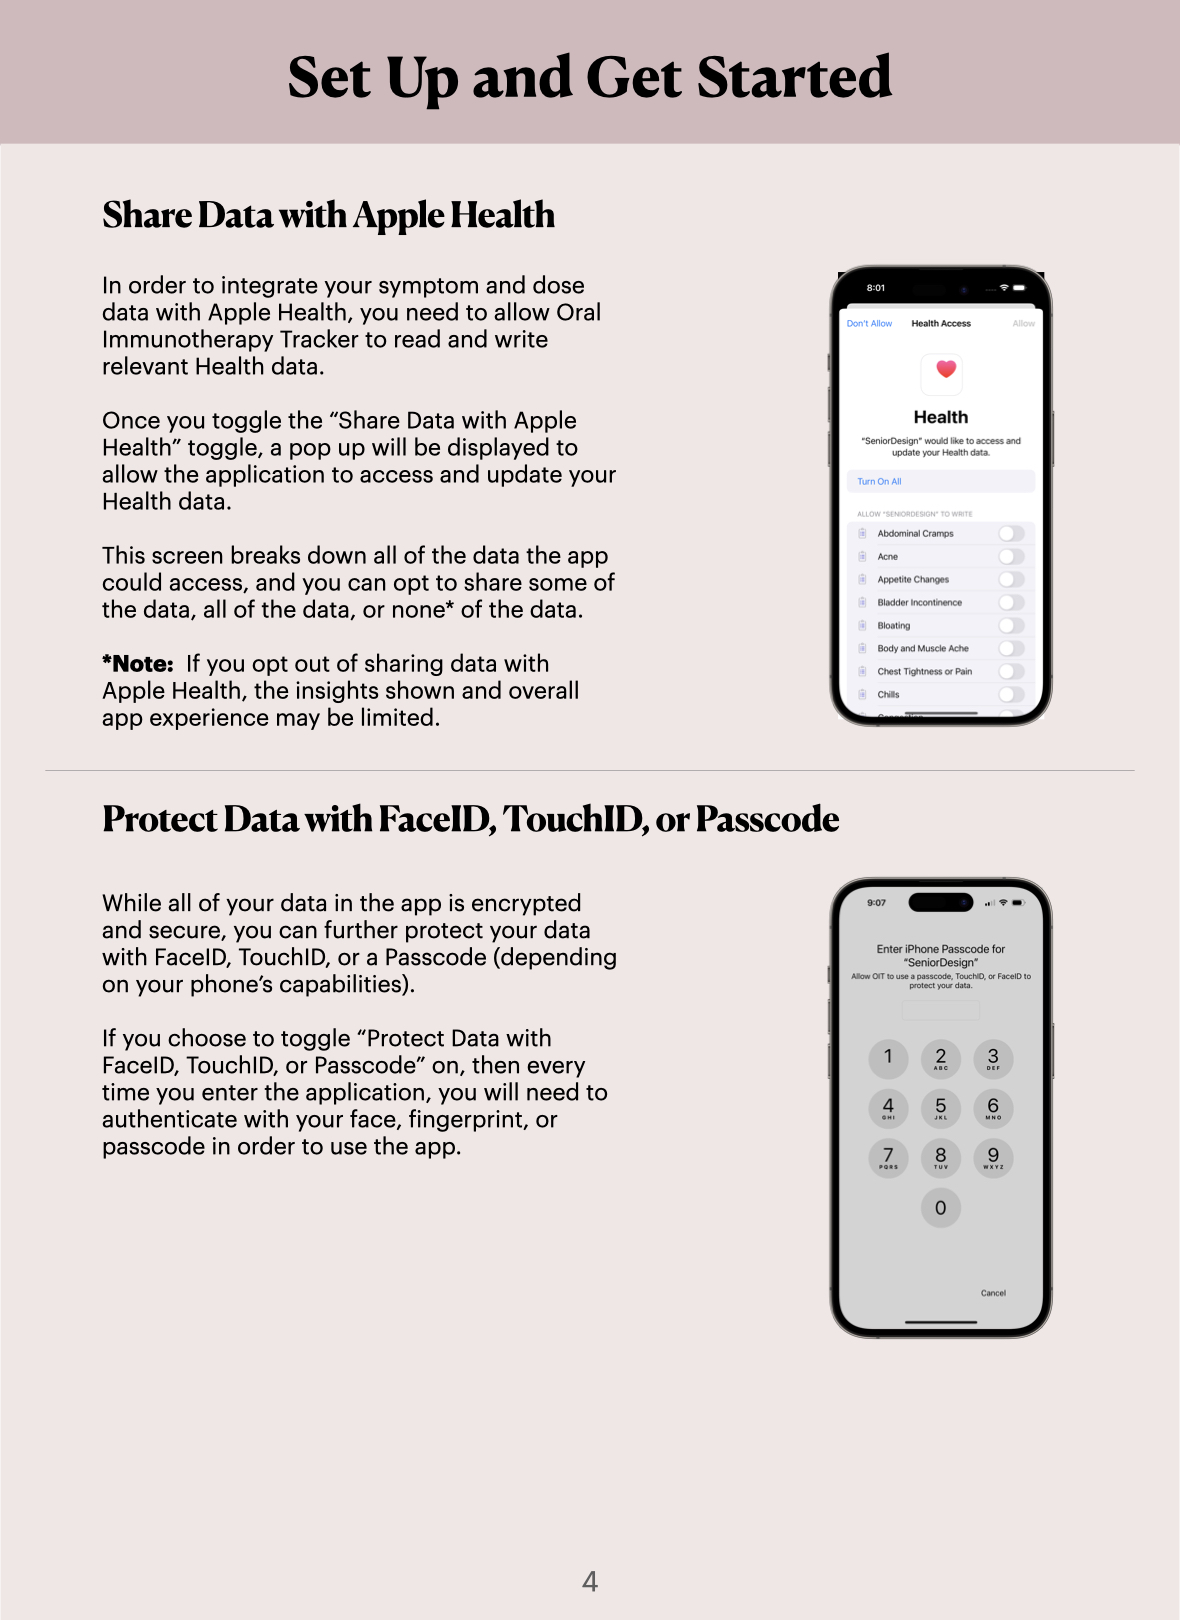
\includegraphics[width=1\linewidth]{thesis//chapters//images/User Guide.004.jpeg}
    \caption{User Guide Page 4}
    \label{fig:enter-label}
\end{figure}

\begin{figure} [H]
    \centering
    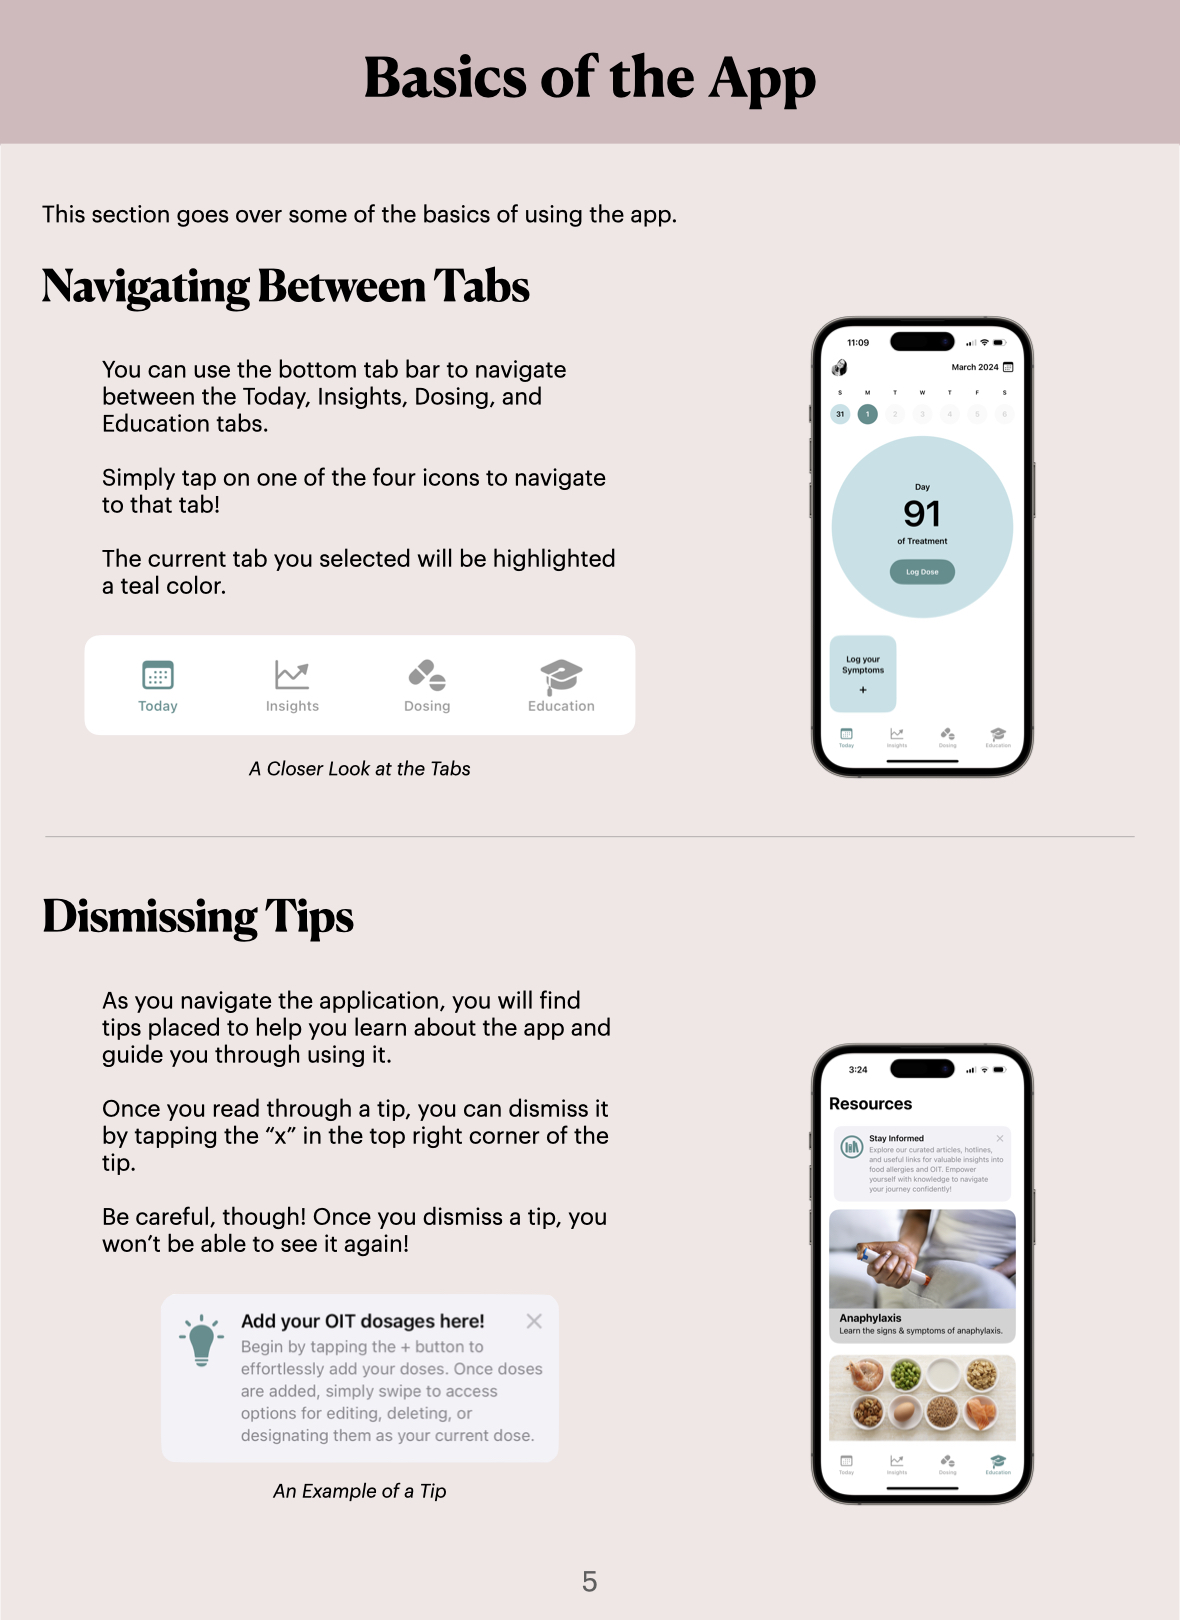
\includegraphics[width=1\linewidth]{thesis//chapters//images/User Guide.005.jpeg}
    \caption{User Guide Page 5}
    \label{fig:enter-label}
\end{figure}

\begin{figure} [H]
    \centering
    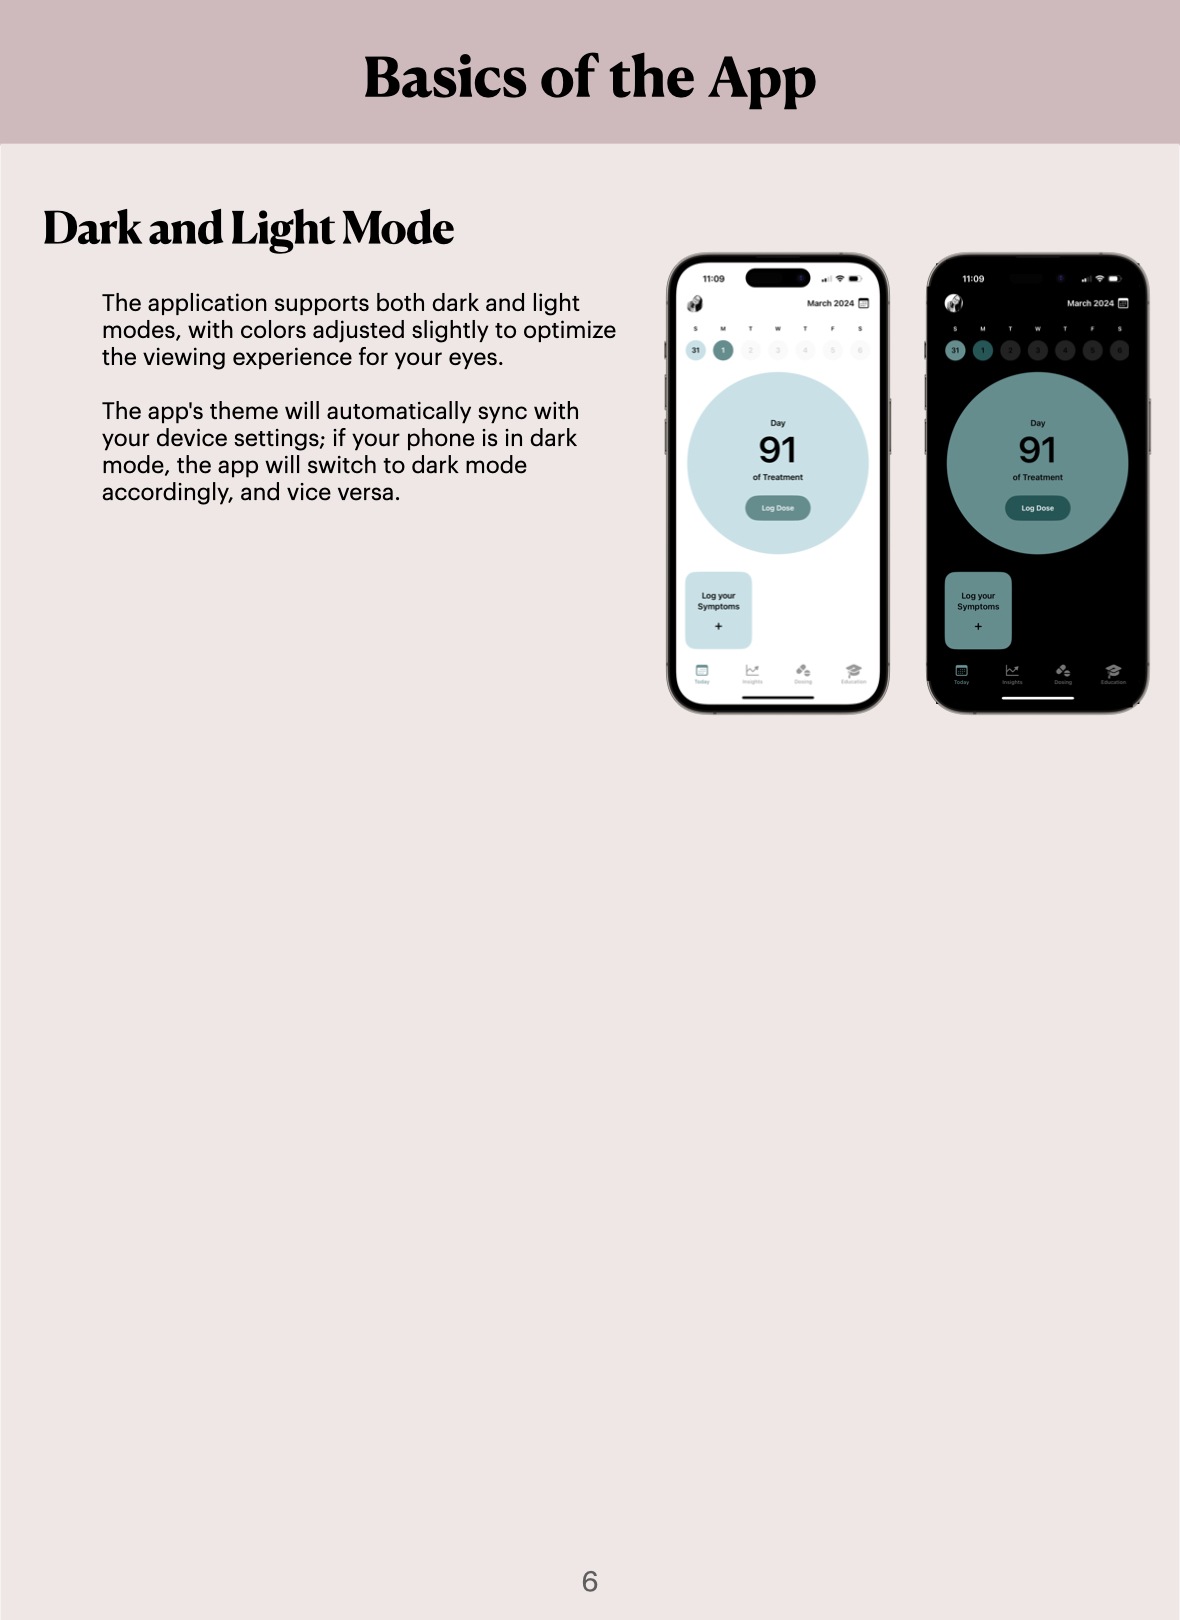
\includegraphics[width=1\linewidth]{thesis//chapters//images/User Guide.006.jpeg}
    \caption{User Guide Page 6}
    \label{fig:enter-label}
\end{figure}

\begin{figure} [H]
    \centering
    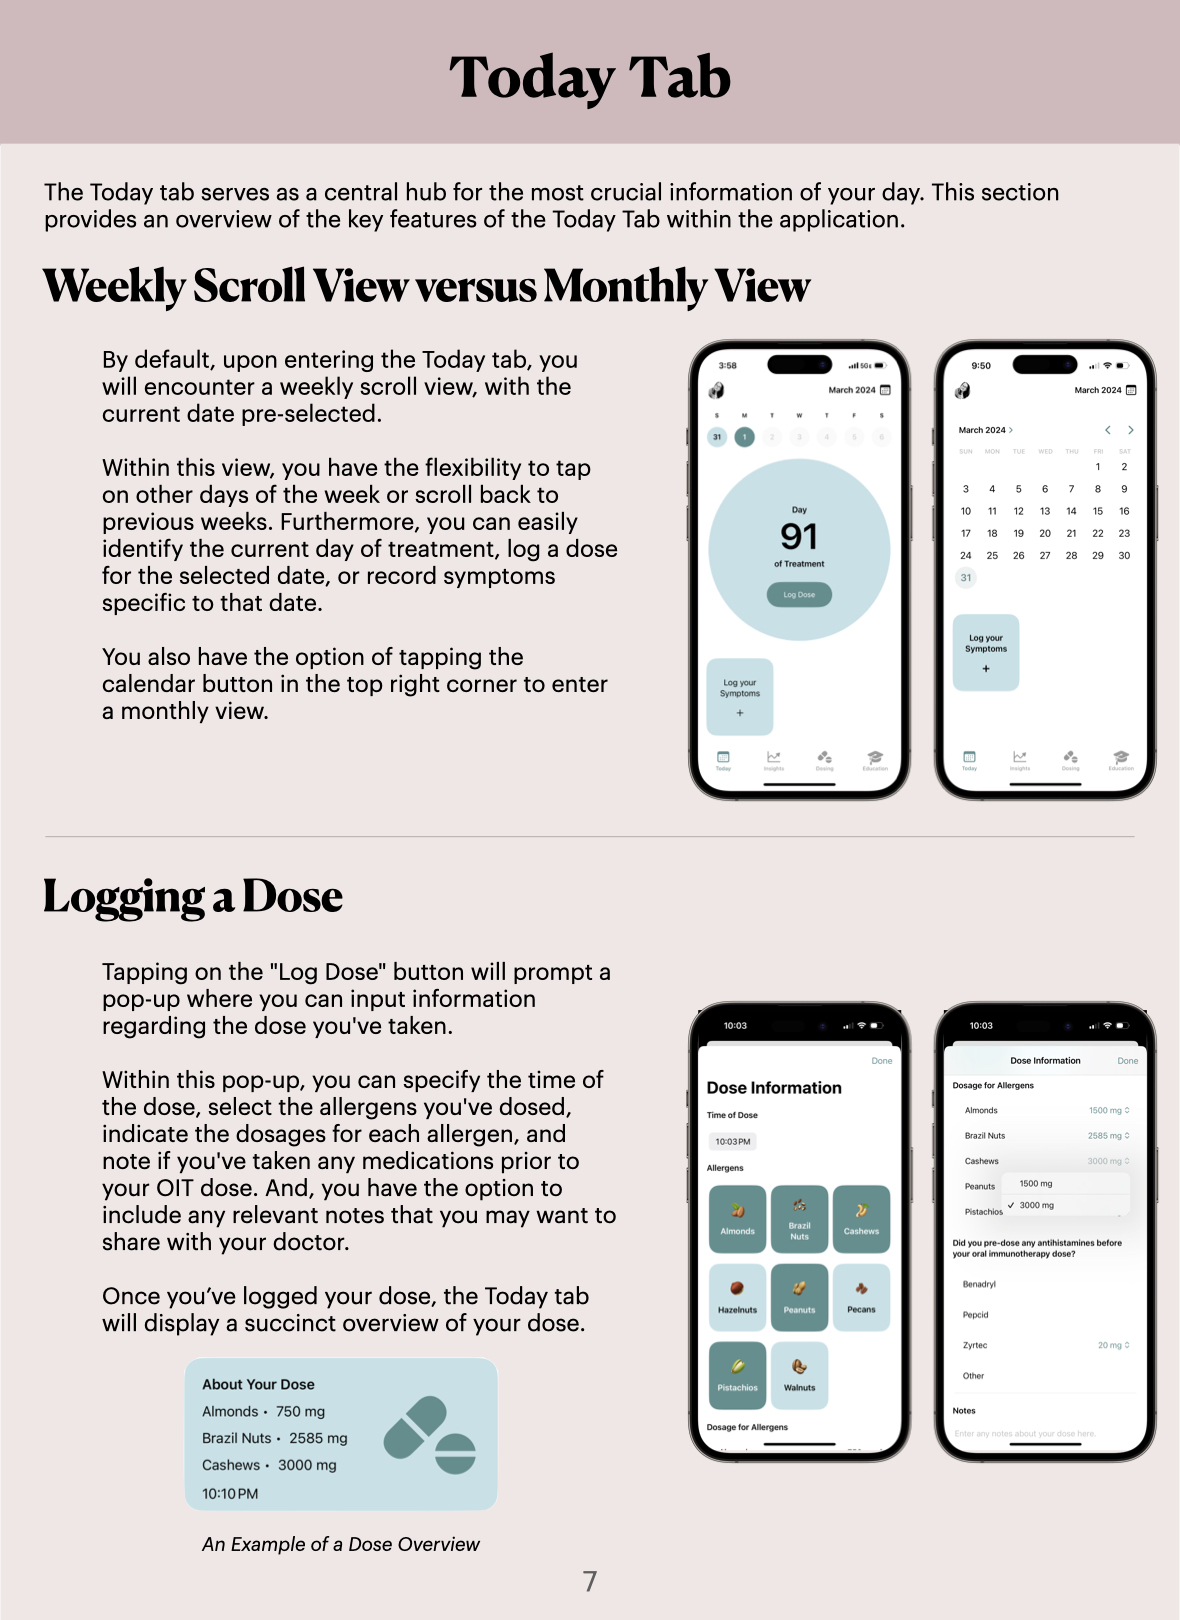
\includegraphics[width=1\linewidth]{thesis//chapters//images/User Guide.007.jpeg}
    \caption{User Guide Page 7}
    \label{fig:enter-label}
\end{figure}

\begin{figure} [H]
    \centering
    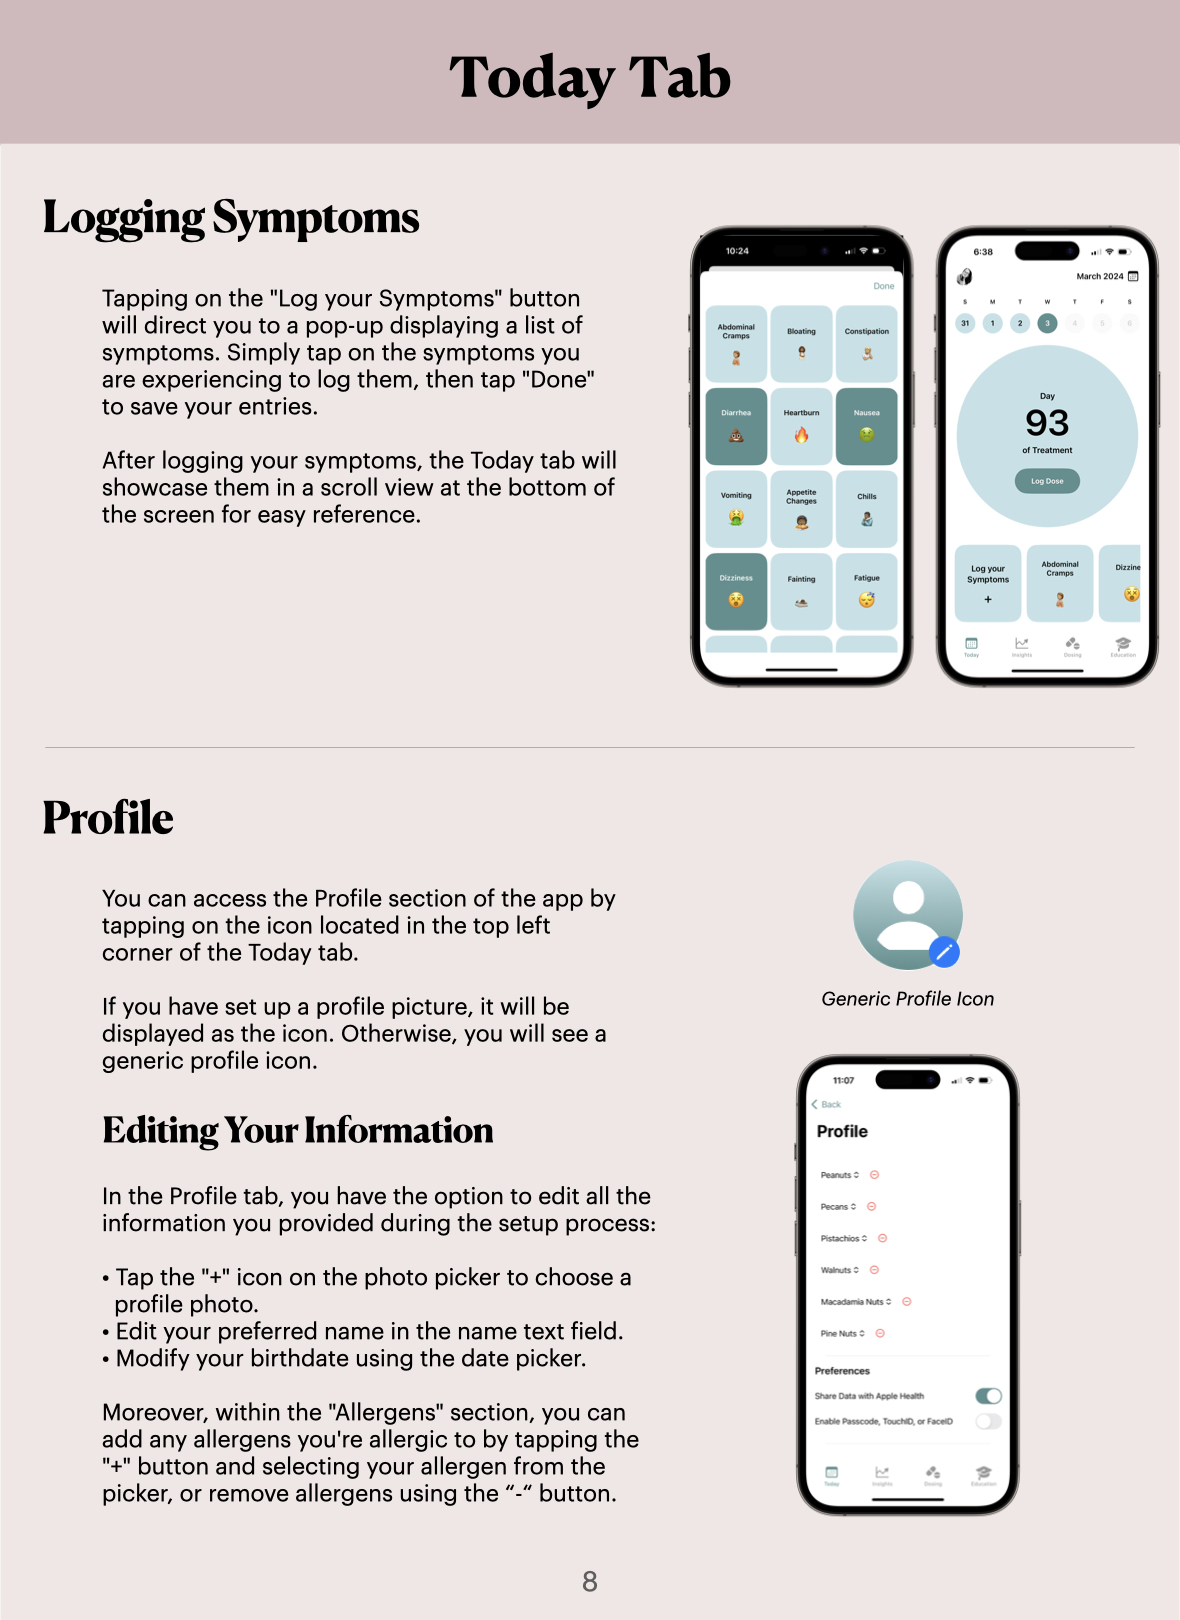
\includegraphics[width=1\linewidth]{thesis//chapters//images/User Guide.008.jpeg}
    \caption{User Guide Page 8}
    \label{fig:enter-label}
\end{figure}

\begin{figure} [H]
    \centering
    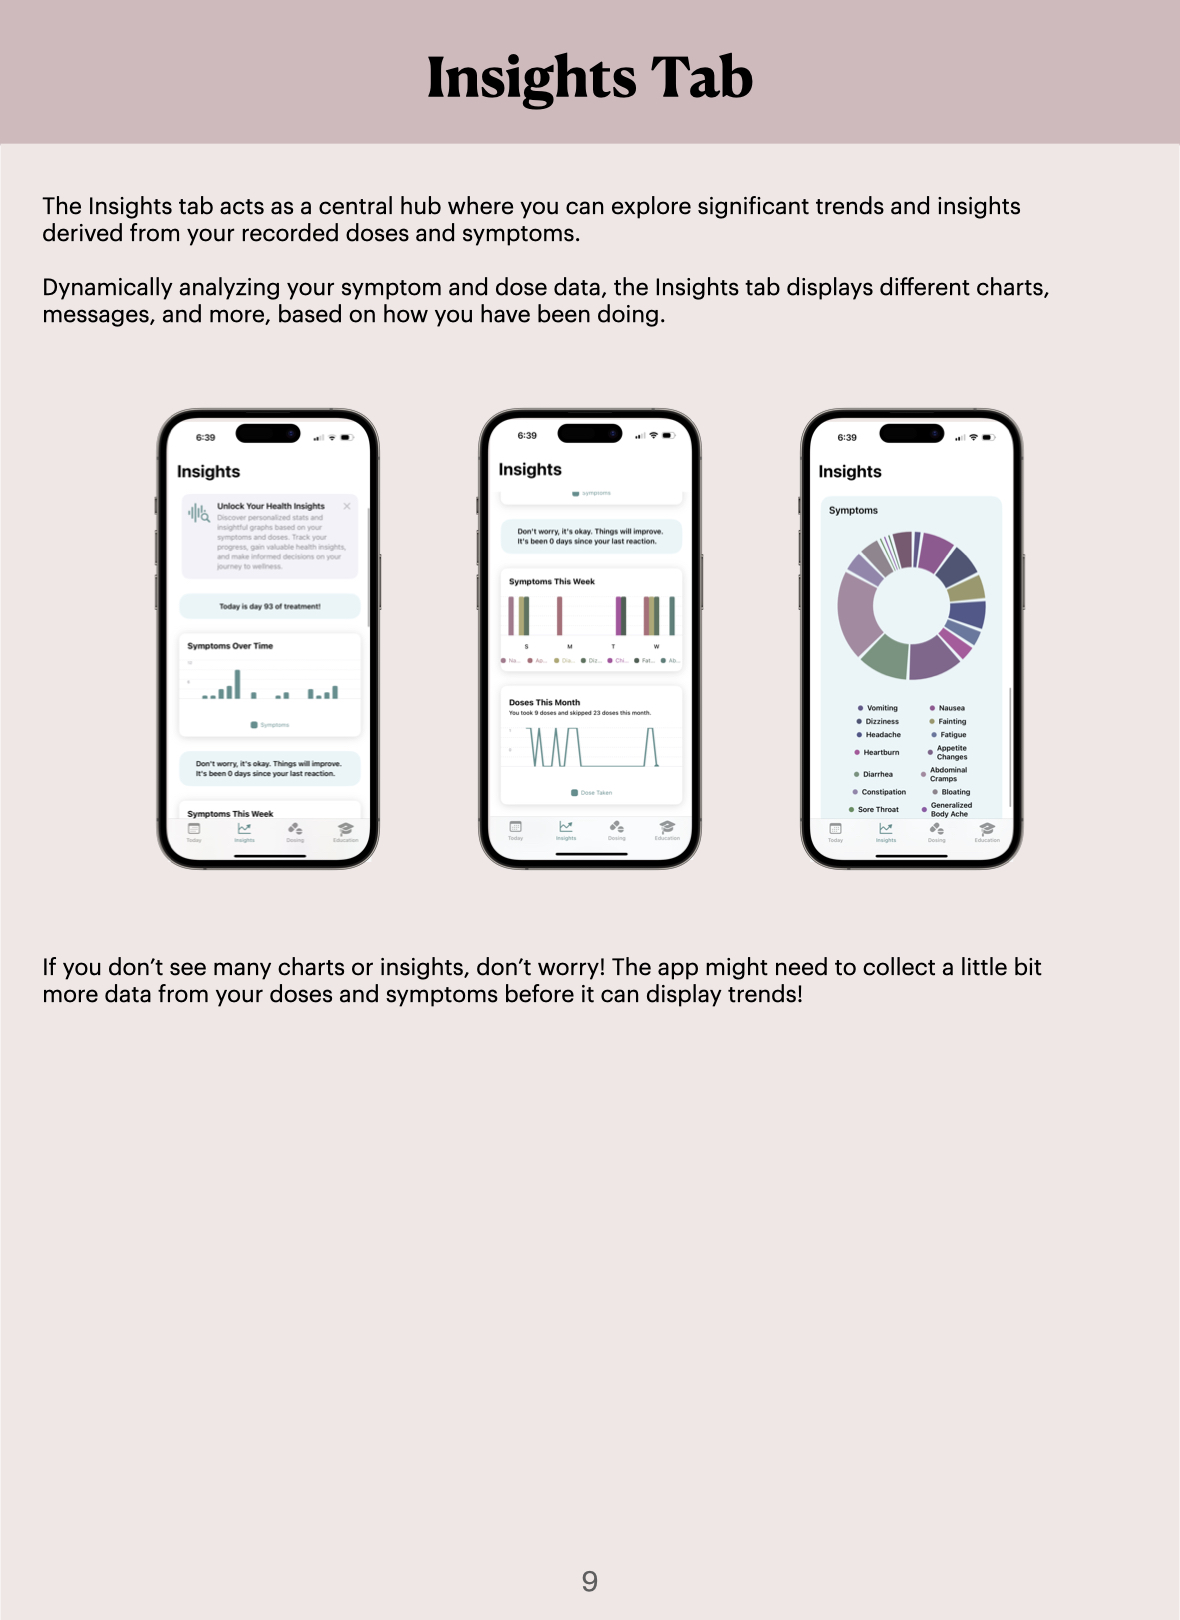
\includegraphics[width=1\linewidth]{thesis//chapters//images/User Guide.009.jpeg}
    \caption{User Guide Page 9}
    \label{fig:enter-label}
\end{figure}

\begin{figure} [H]
    \centering
    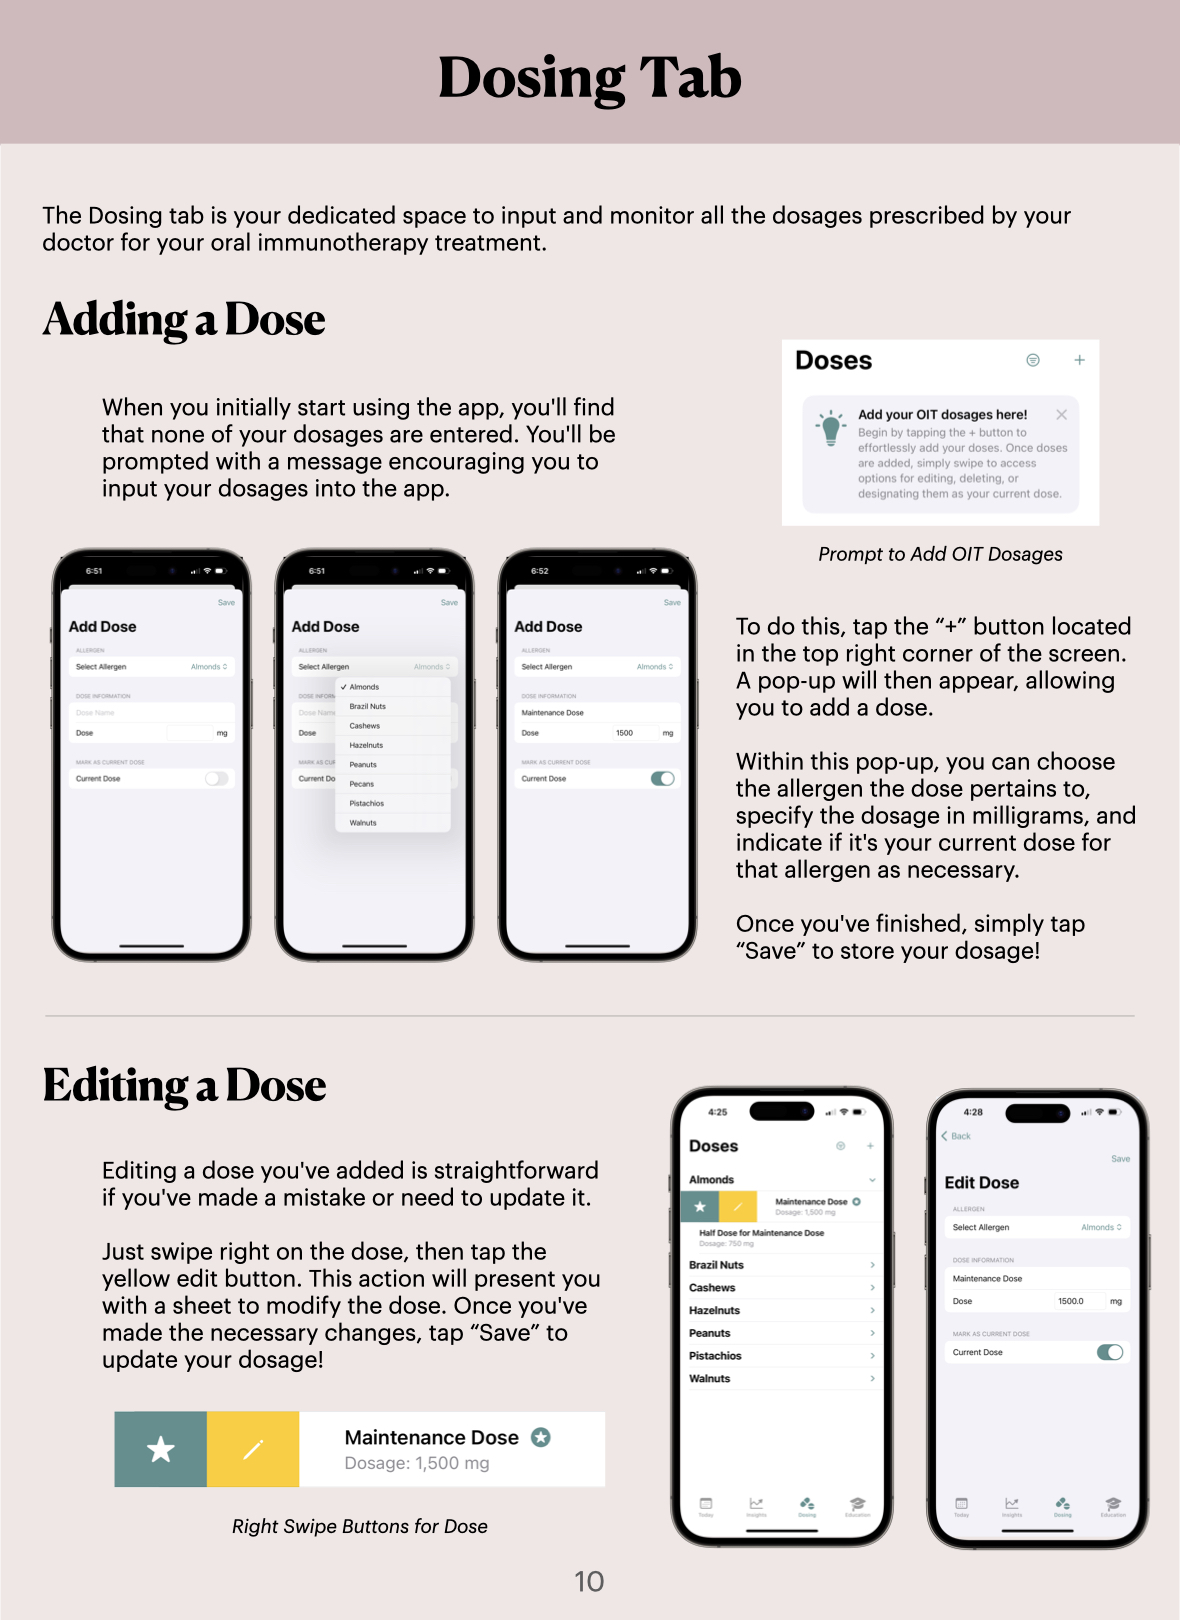
\includegraphics[width=1\linewidth]{thesis//chapters//images/User Guide.010.jpeg}
    \caption{User Guide Page 10}
    \label{fig:enter-label}
\end{figure}

\begin{figure} [H]
    \centering
    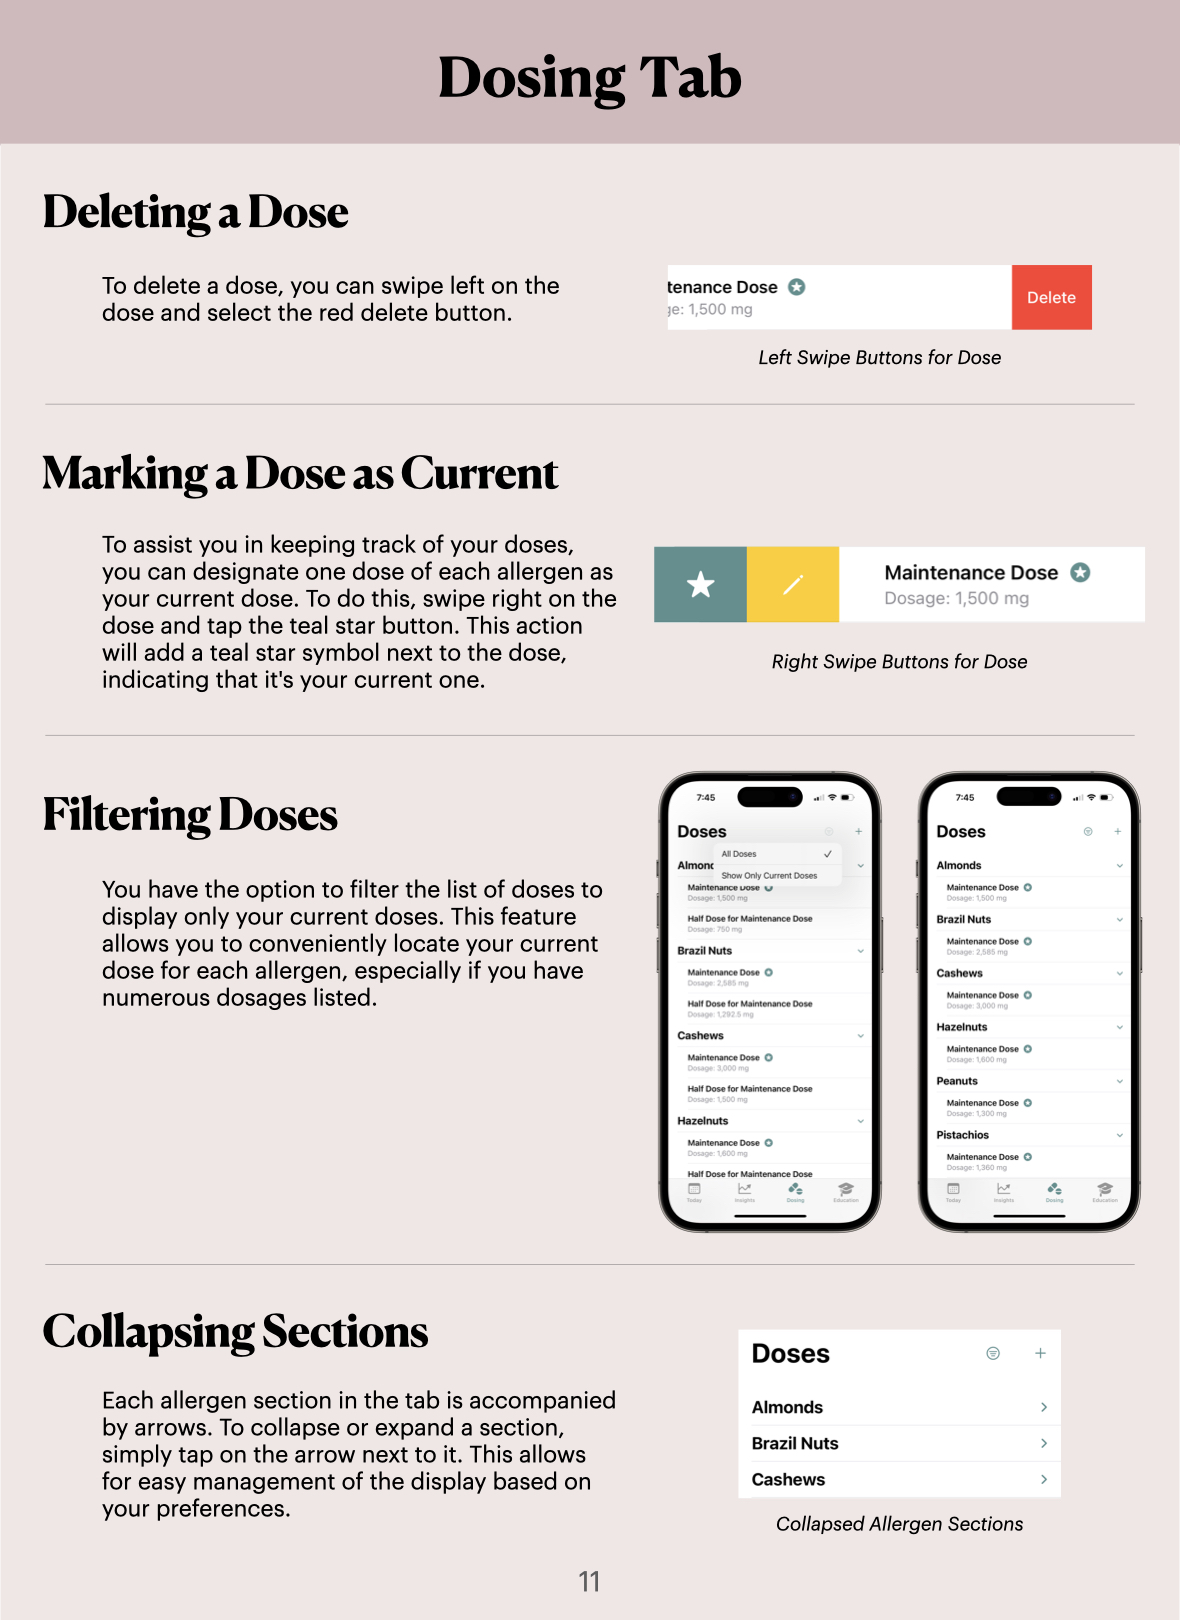
\includegraphics[width=1\linewidth]{thesis//chapters//images/User Guide.011.jpeg}
    \caption{User Guide Page 11}
    \label{fig:enter-label}
\end{figure}

\begin{figure} [H]
    \centering
    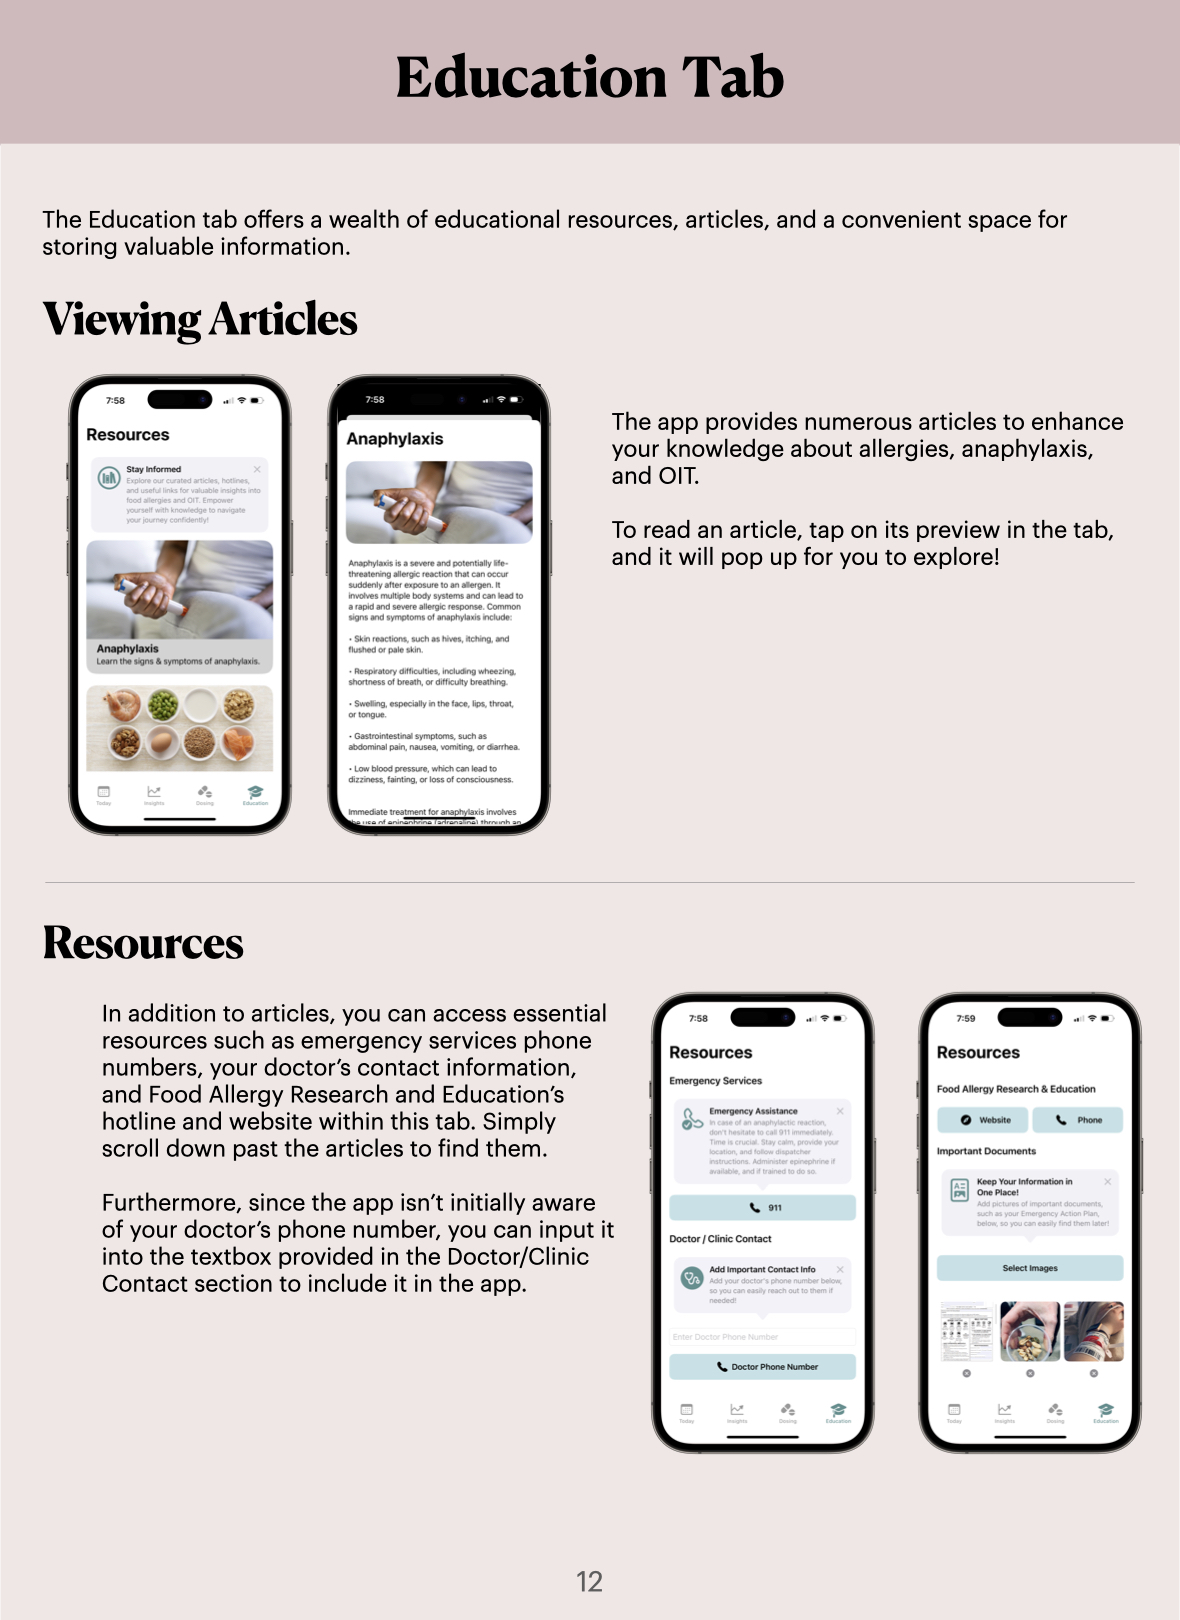
\includegraphics[width=1\linewidth]{thesis//chapters//images/User Guide.012.jpeg}
    \caption{User Guide Page 12}
    \label{fig:enter-label}
\end{figure}

\begin{figure} [H]
    \centering
    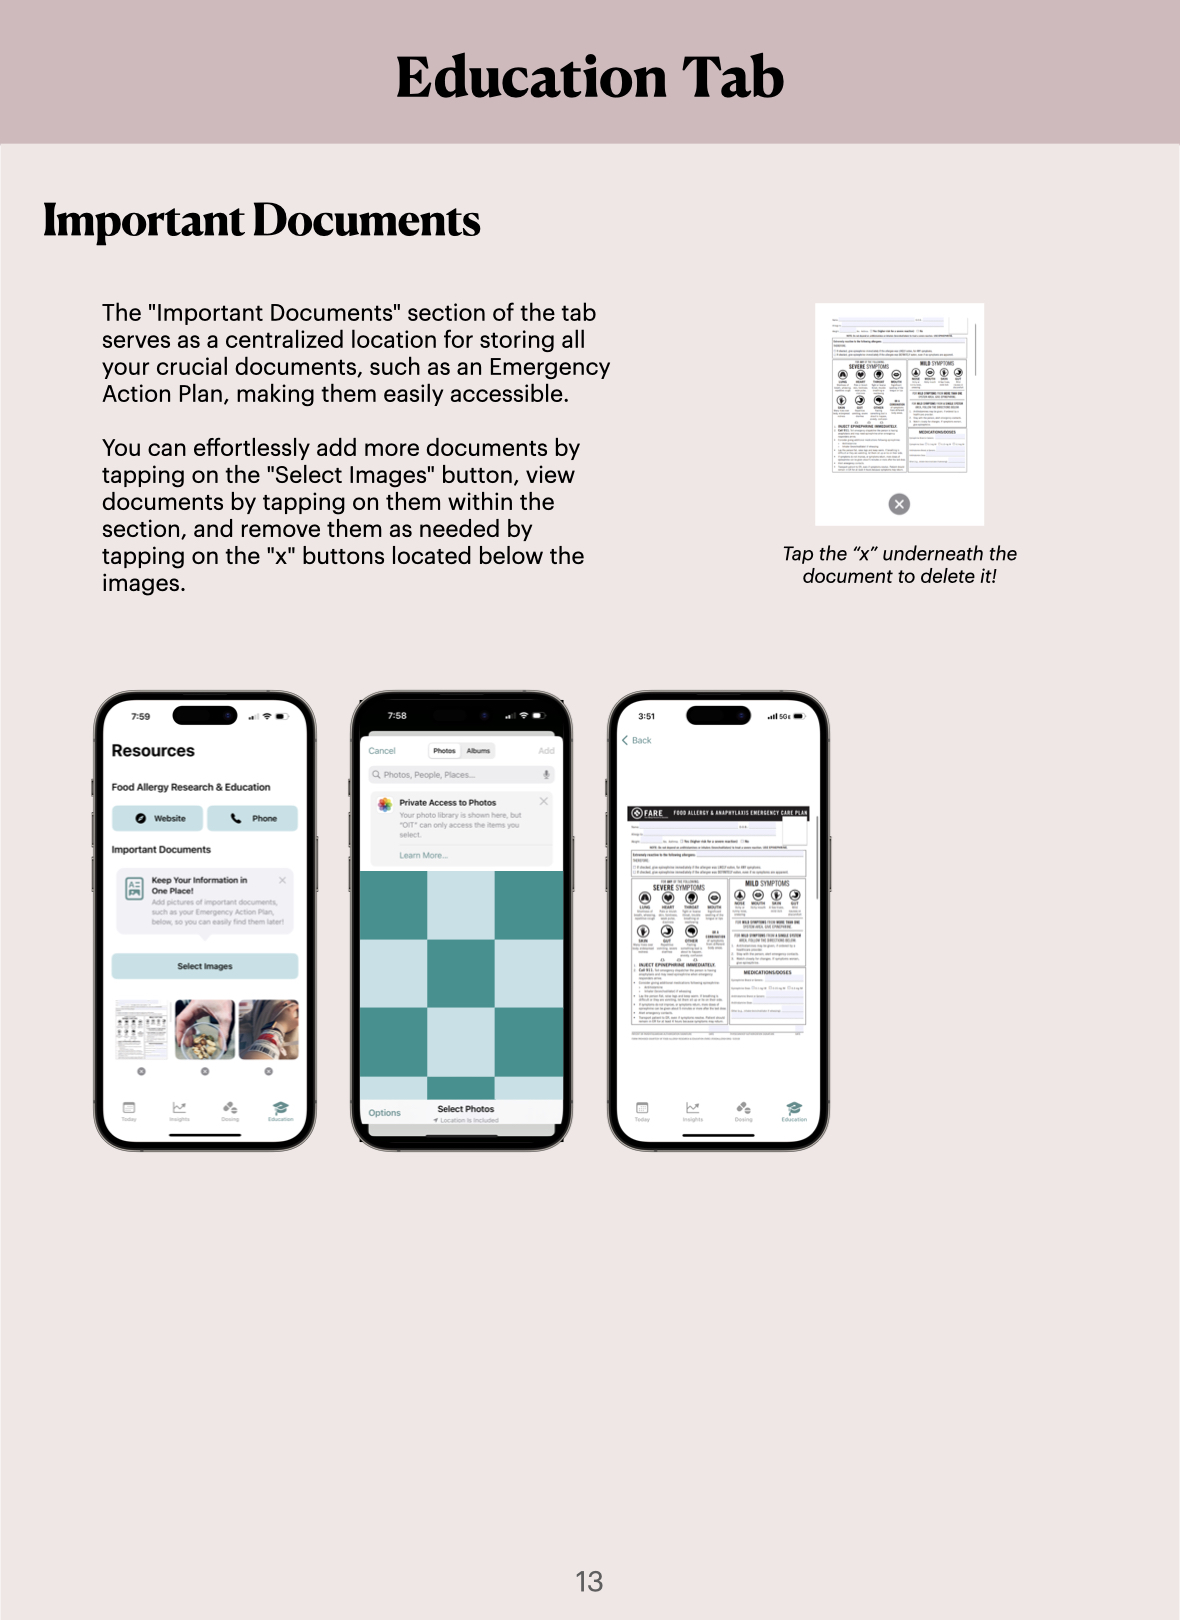
\includegraphics[width=1\linewidth]{thesis//chapters//images/User Guide.013.jpeg}
    \caption{User Guide Page 13}
    \label{fig:enter-label}
\end{figure}

\begin{figure} [H]
    \centering
    
\includegraphics[width=1\linewidth]{thesis//chapters//images/User Guide.014.jpeg}
    \caption{User Guide Page 14}
    \label{fig:enter-label}
\end{figure}

